\documentclass{article}
\usepackage{graphicx}
\usepackage{geometry}
\usepackage{hyperref}
\usepackage{booktabs}
\usepackage{subcaption}
\usepackage{amsmath}
\usepackage{amssymb}

\geometry{a4paper, margin=0.65in}

\hypersetup{
    colorlinks=true,
    linkcolor=blue,
    filecolor=magenta,
    urlcolor=cyan,
}

\title{Gradient-Preserving Activation Clipping: MNIST Report}
\author{ByzFL SNN Benchmark}
\date{\today}

\begin{document}

\maketitle

\clearpage
\tableofcontents
\clearpage

\section{Activation Definitions}

All variants below share the same MNIST CNN architecture
(\texttt{Conv2d(1,20,5,1)} $\to$ \texttt{Conv2d(20,50,5,1)} $\to$ \texttt{Linear(800,500)}
$\to$ \texttt{Linear(500,10)}), differing only in the activation applied after the first
three layers (the final layer always uses \texttt{log\_softmax}). Forward/backward
definitions below are transcribed directly from
\texttt{byzfl/fed\_framework/clipped\_activations.py} and
\texttt{byzfl/fed\_framework/client.py}.

\subsection{Baseline: Hardtanh Clip (existing, true derivative)}
Forward and backward are both the standard \texttt{hardtanh} clamp -- the gradient
genuinely vanishes above the clip value:
\begin{align*}
    y &= \mathrm{clamp}(x, 0, C) \\
    \frac{\partial y}{\partial x} &=
    \begin{cases}
        1 & 0 < x < C \\
        0 & \text{otherwise}
    \end{cases}
\end{align*}

\subsection{STE Clip (\texttt{ClippedReLU\_STE})}
Forward is the same hard clamp; the backward pass is a straight-through estimator that
never zeroes the gradient for positive inputs, regardless of saturation:
\begin{align*}
    y &= \mathrm{clamp}(x, 0, C) \\
    \frac{\partial y}{\partial x} &=
    \begin{cases}
        1 & x > 0 \\
        0 & x \leq 0
    \end{cases}
\end{align*}

\subsection{Ramp Clip (\texttt{ClippedReLU\_Ramp})}
Forward is the same hard clamp to $[0, C]$. The backward pass keeps slope $1$ up to
$C$, then decays \emph{linearly} to $0$ over $[C, rC]$ (ramp ratio $r$; $r=2$ in all
runs here, so the ramp ends at $2C$) -- this preserves the distinction between a
coordinate that is slightly over $C$ and one that is far over $C$, instead of treating
both identically:
\begin{align*}
    y &= \mathrm{clamp}(x, 0, C) \\
    \frac{\partial y}{\partial x} &=
    \begin{cases}
        1 & 0 < x \leq C \\
        \dfrac{rC - x}{rC - C} & C < x < rC \\
        0 & x \leq 0 \ \text{or}\ x \geq rC
    \end{cases}
\end{align*}

\subsection{Fixed Gradient-Norm Clip (\texttt{gradient\_clip\_val}$=21$)}
Also not an activation function -- a plain-ReLU CNN where each honest client's overall
gradient (all parameters concatenated) is rescaled, via
\texttt{torch.nn.utils.clip\_grad\_norm\_}, to a fixed global L2 norm threshold
$C_g = 21$, applied to the raw per-parameter \texttt{.grad} tensors right after
\texttt{loss.backward()} -- i.e.\ before flattening and before the momentum
accumulation described below:
\begin{align*}
    g &= \nabla_\theta \mathcal{L}(\theta) \quad \text{(concatenation of all parameter gradients)} \\
    g^{\text{clipped}} &=
    \begin{cases}
        g \cdot \dfrac{C_g}{\lVert g \rVert_2} & \lVert g \rVert_2 > C_g \\
        g & \text{otherwise}
    \end{cases}
\end{align*}
Unlike the adaptive client-side clip below, $C_g$ is a fixed constant (not
data-adaptive) and is not a quantile of anything.

\subsection{Adaptive Per-Coordinate Quantile Clip (\texttt{AdaptiveQuantileClip})}
Instead of a fixed constant $C$, the clip threshold is recomputed every forward pass as
the $\tau$-quantile of that layer's own activation coordinates (detached, i.e. treated
as a constant for backpropagation), so the threshold adapts to the current activation
distribution instead of being hand-picked. Two backward variants were implemented --
\emph{plain} (same failure mode as hardtanh: hard zero above $C$) and \emph{STE}
(gradient survives above $C$):
\begin{align*}
    C &= \mathrm{quantile}_\tau\big(\mathrm{flatten}(x)\big) \quad \text{(detached)} \\
    y &= \mathrm{clamp}(x, 0, C) \\
    \frac{\partial y}{\partial x} &=
    \begin{cases}
        \mathbb{1}[0 < x \leq C] & \text{plain} \\
        \mathbb{1}[x > 0] & \text{STE}
    \end{cases}
\end{align*}
Swept at $\tau \in \{0.80, 0.90\}$, both backward variants
(\emph{results pending -- not yet available at time of writing}).

\subsection{Adaptive Client-Side Gradient-Norm Clip}
Not an activation function -- a plain-ReLU CNN where each honest client clips the L2
norm of the (post-momentum) gradient vector it sends to the server, to the
$\tau$-quantile of its own last $W=100$ gradient norms (a sliding window, since
gradient norms are non-stationary and shrink over training). Let $v_t$ be the momentum
gradient at step $t$ and $n_t = \lVert v_t \rVert_2$; a history buffer of the last $W$
values of $n_t$ is maintained \emph{before} any clipping is applied, so the quantile
reflects the true, unclipped distribution:
\begin{align*}
    \tau\text{-threshold}_t &= \mathrm{quantile}_\tau\big(\{n_{t-W+1}, \dots, n_t\}\big) \\
    v_t^{\text{sent}} &=
    \begin{cases}
        v_t \cdot \dfrac{\tau\text{-threshold}_t}{n_t} & n_t > \tau\text{-threshold}_t \\
        v_t & \text{otherwise}
    \end{cases}
\end{align*}
The internal momentum buffer itself is never rescaled -- only the copy actually sent to
the server is clipped. Swept at $\tau \in \{0.70, 0.80\}$
(\emph{results pending -- not yet available at time of writing}).

\clearpage
\section{Best Overall Performance (Worst-Case Across Attacks)}
\begin{figure}[htbp]
    \centering
    \begin{subfigure}[b]{0.32\textwidth}
        \centering
        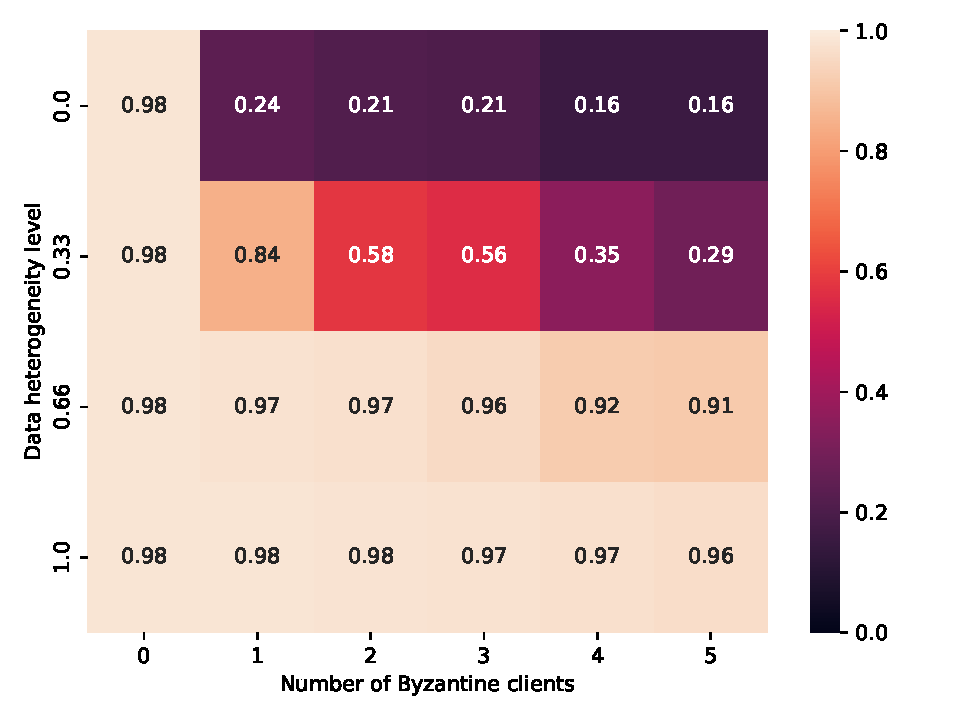
\includegraphics[width=\textwidth]{../plots/mnist_clipping_heatmaps/cnn_mnist/best_test_mnist_cnn_mnist_gamma_similarity_niid_NNM_ARC_nb_honest_clients_10_tolerated_f_equal_real.pdf}
        \caption{No Clip (ReLU)}
        \label{fig:best_overall_noclip}
    \end{subfigure}
    \hfill
    \begin{subfigure}[b]{0.32\textwidth}
        \centering
        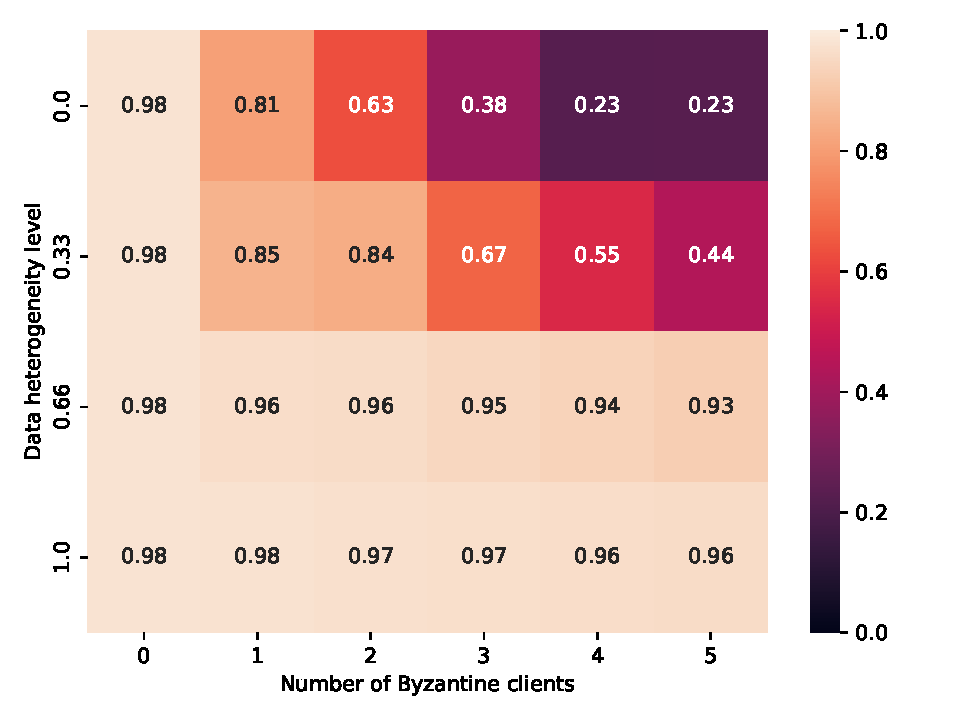
\includegraphics[width=\textwidth]{../plots/cnn_tanh_heatmaps/best_test_mnist_cnn_mnist_tanh_gamma_similarity_niid_NNM_ARC_nb_honest_clients_10_tolerated_f_equal_real.pdf}
        \caption{Tanh}
        \label{fig:best_overall_tanh}
    \end{subfigure}
    \hfill
    \begin{subfigure}[b]{0.32\textwidth}
        \centering
        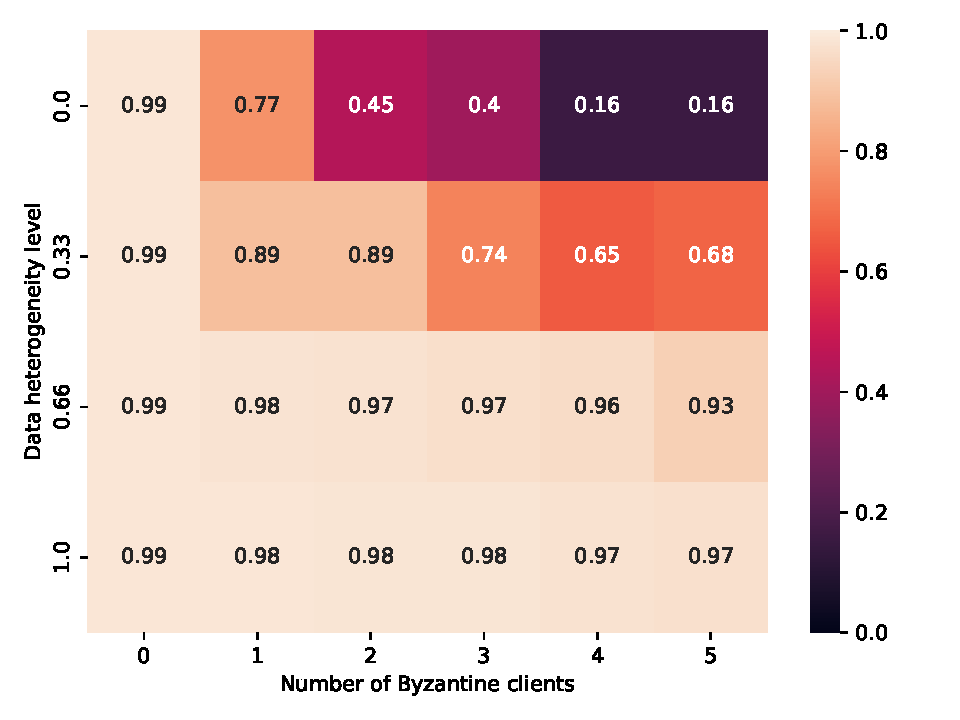
\includegraphics[width=\textwidth]{../plots/cnn_clipped_heatmaps/best_test_mnist_cnn_mnist_gamma_similarity_niid_NNM_ARC_nb_honest_clients_10_tolerated_f_equal_real.pdf}
        \caption{Grad-Norm Clip $=21$}
        \label{fig:best_overall_gradnorm21}
    \end{subfigure}
    \vspace{0.3cm}
    \begin{subfigure}[b]{0.32\textwidth}
        \centering
        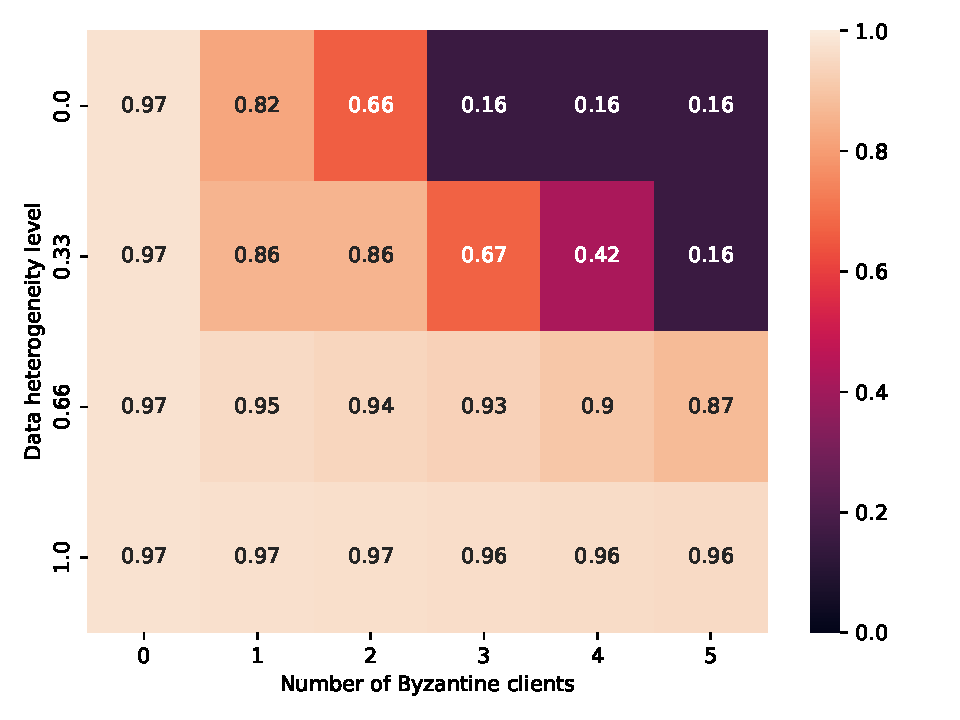
\includegraphics[width=\textwidth]{../plots/mnist_clipping_heatmaps/cnn_mnist_clipping_1/best_test_mnist_cnn_mnist_clipping_1_gamma_similarity_niid_NNM_ARC_nb_honest_clients_10_tolerated_f_equal_real.pdf}
        \caption{Hardtanh $C{=}1$}
        \label{fig:best_overall_hardtanh_1}
    \end{subfigure}
    \hfill
    \begin{subfigure}[b]{0.32\textwidth}
        \centering
        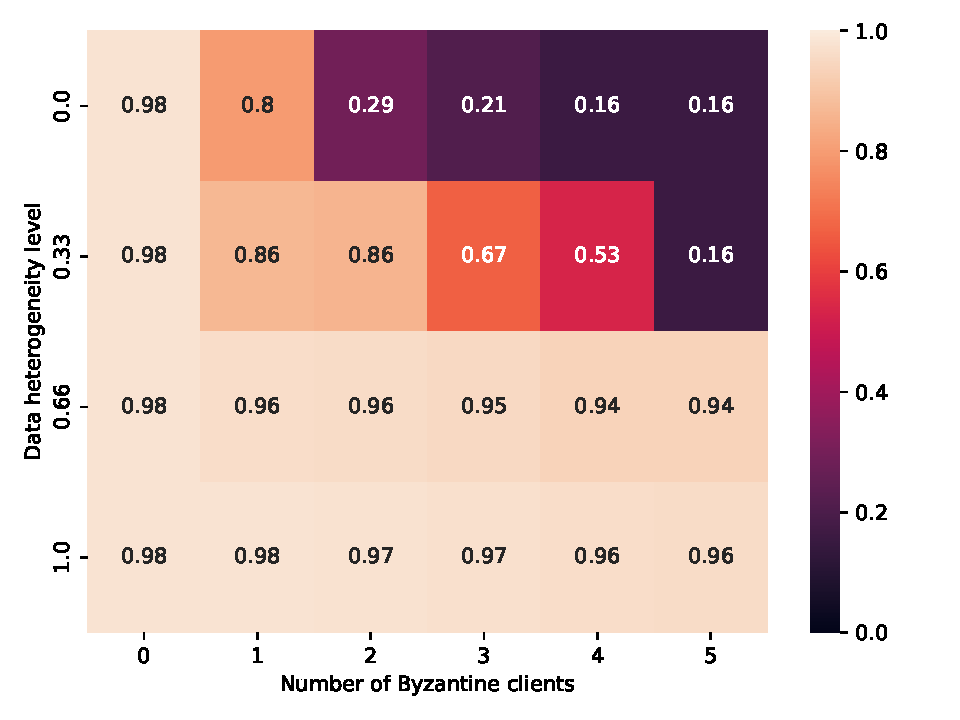
\includegraphics[width=\textwidth]{../plots/mnist_clipping_heatmaps/cnn_mnist_clipping_2/best_test_mnist_cnn_mnist_clipping_2_gamma_similarity_niid_NNM_ARC_nb_honest_clients_10_tolerated_f_equal_real.pdf}
        \caption{Hardtanh $C{=}2$}
        \label{fig:best_overall_hardtanh_2}
    \end{subfigure}
    \hfill
    \begin{subfigure}[b]{0.32\textwidth}
        \centering
        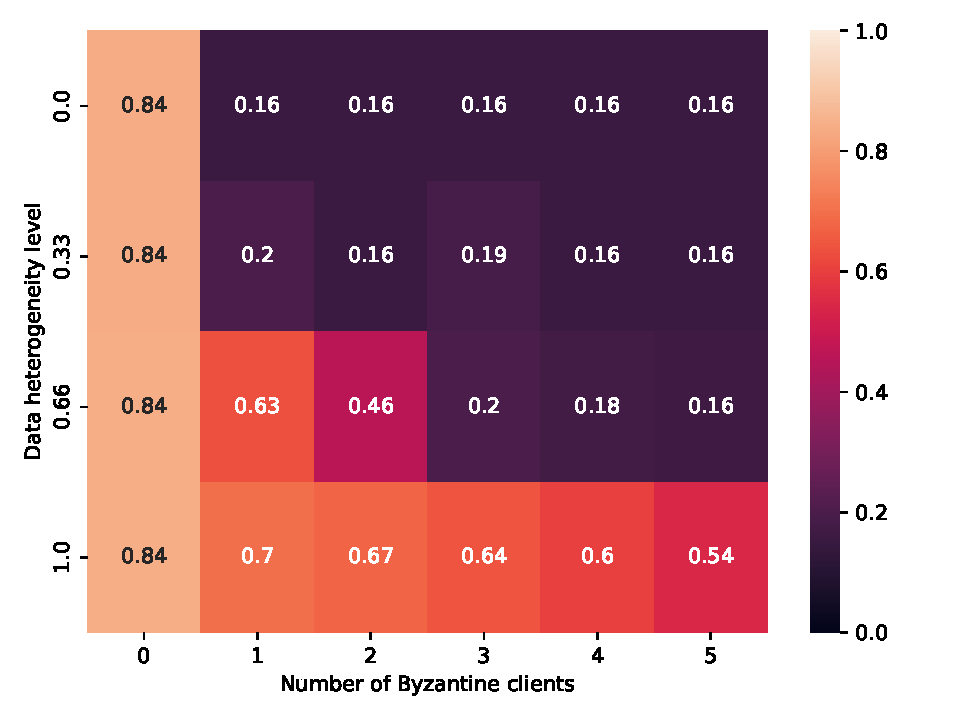
\includegraphics[width=\textwidth]{../activation_clip_plots/cnn_mnist_clip_ste_1/best_test_mnist_cnn_mnist_clip_ste_1_gamma_similarity_niid_NNM_ARC_nb_honest_clients_10_tolerated_f_equal_real.pdf}
        \caption{STE $C{=}1$}
        \label{fig:best_overall_ste_1}
    \end{subfigure}
    \vspace{0.3cm}
    \begin{subfigure}[b]{0.32\textwidth}
        \centering
        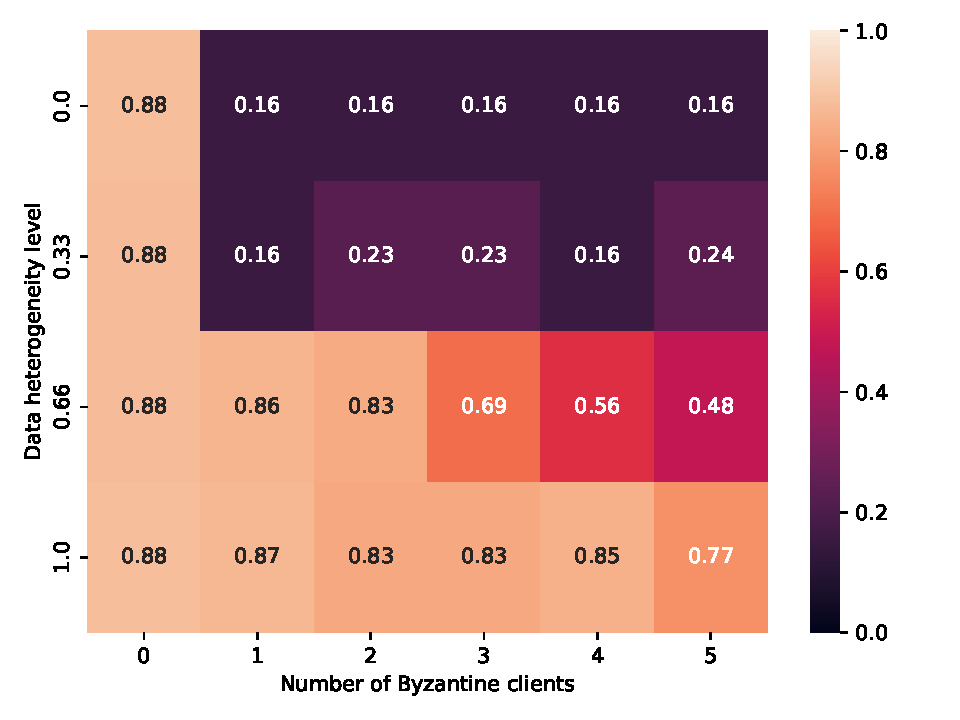
\includegraphics[width=\textwidth]{../activation_clip_plots/cnn_mnist_clip_ste_2/best_test_mnist_cnn_mnist_clip_ste_2_gamma_similarity_niid_NNM_ARC_nb_honest_clients_10_tolerated_f_equal_real.pdf}
        \caption{STE $C{=}2$}
        \label{fig:best_overall_ste_2}
    \end{subfigure}
    \hfill
    \begin{subfigure}[b]{0.32\textwidth}
        \centering
        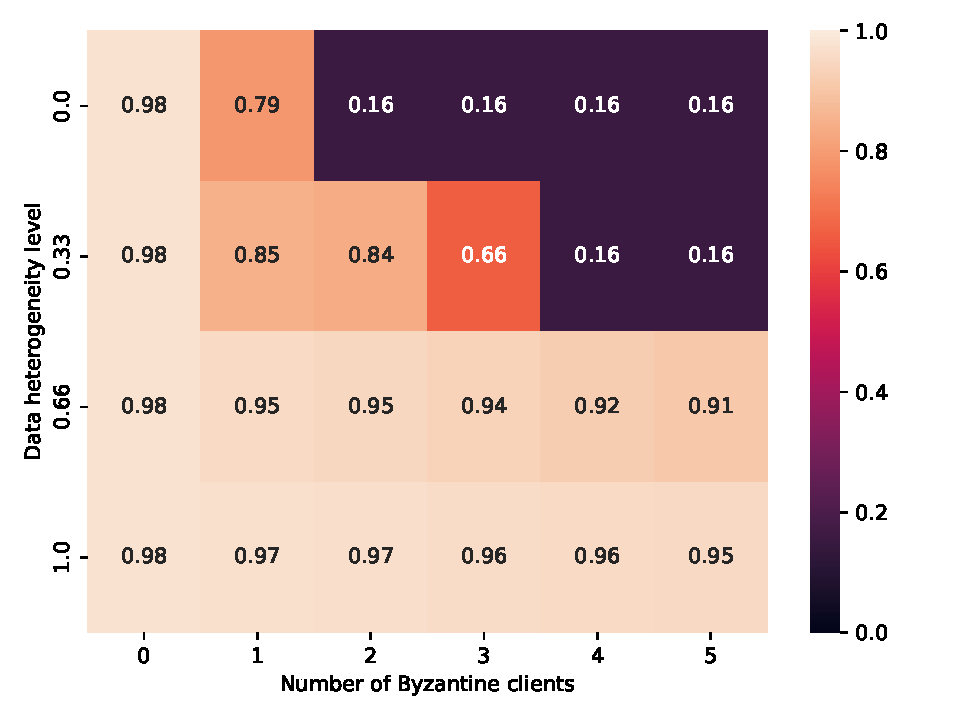
\includegraphics[width=\textwidth]{../activation_clip_plots/cnn_mnist_clip_ramp_1/best_test_mnist_cnn_mnist_clip_ramp_1_gamma_similarity_niid_NNM_ARC_nb_honest_clients_10_tolerated_f_equal_real.pdf}
        \caption{Ramp $C{=}1$ ($r{=}2$)}
        \label{fig:best_overall_ramp_1}
    \end{subfigure}
    \caption{Best overall test accuracy (worst-case across attacks).}
    \label{fig:best_overall_grid}
\end{figure}
\clearpage
\section{Best Aggregator under Specific Attacks}

\subsection{Optimal ALIE Attack}
\begin{figure}[htbp]
    \centering
    \begin{subfigure}[b]{0.32\textwidth}
        \centering
        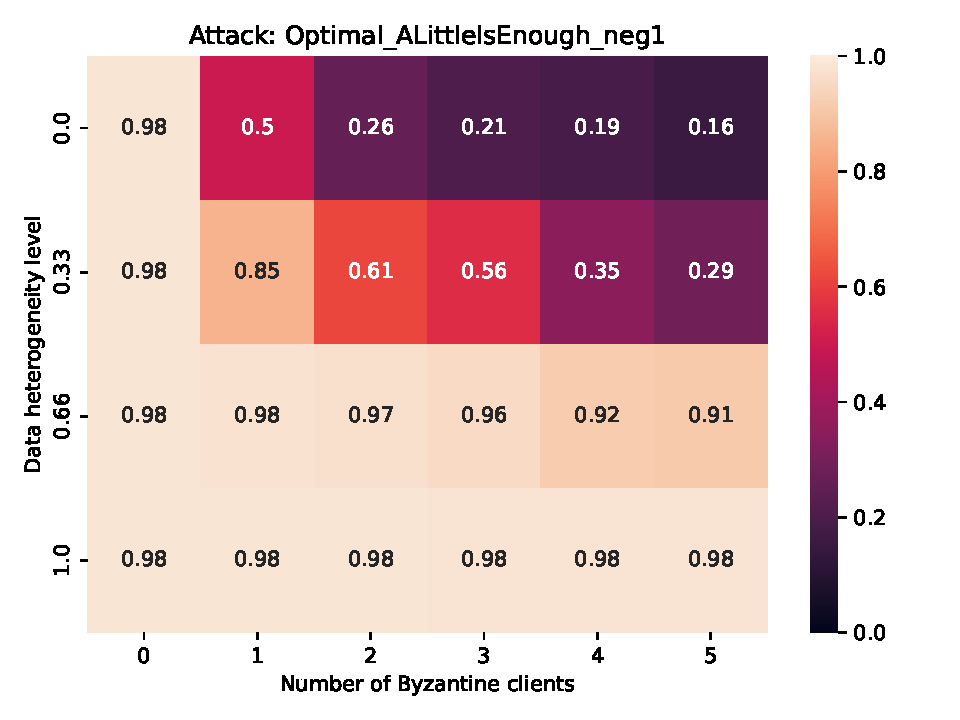
\includegraphics[width=\textwidth]{../plots/mnist_clipping_heatmaps/cnn_mnist/best_test_Optimal_ALittleIsEnough_neg1_mnist_cnn_mnist_gamma_similarity_niid_NNM_ARC_nb_honest_clients_10_tolerated_f_equal_real.pdf}
        \caption{No Clip (ReLU)}
        \label{fig:best_alie_noclip}
    \end{subfigure}
    \hfill
    \begin{subfigure}[b]{0.32\textwidth}
        \centering
        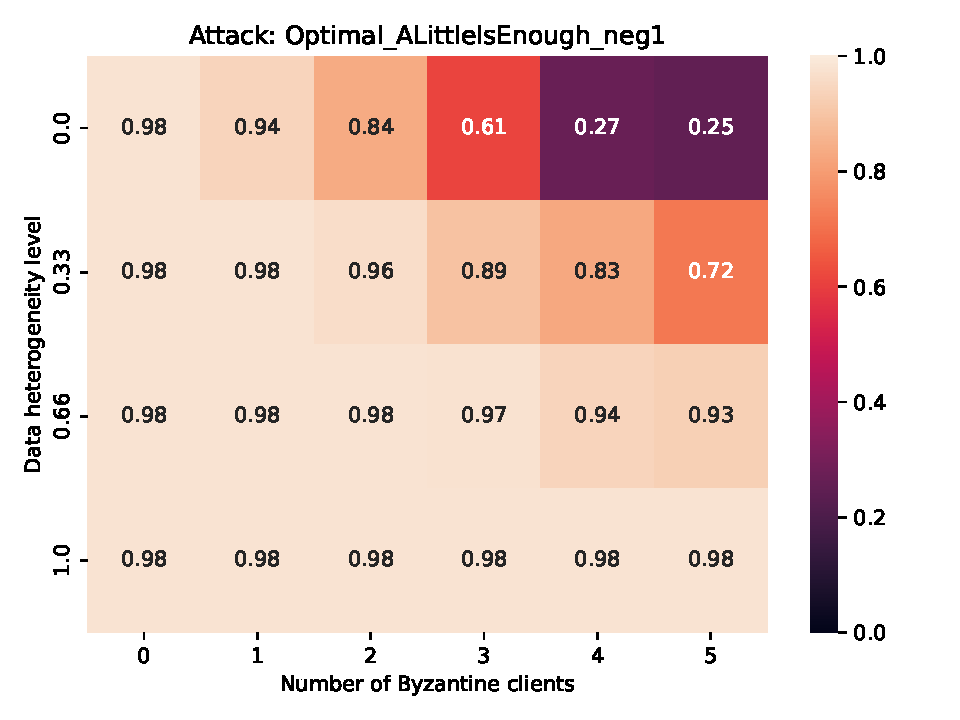
\includegraphics[width=\textwidth]{../plots/cnn_tanh_heatmaps/best_test_Optimal_ALittleIsEnough_neg1_mnist_cnn_mnist_tanh_gamma_similarity_niid_NNM_ARC_nb_honest_clients_10_tolerated_f_equal_real.pdf}
        \caption{Tanh}
        \label{fig:best_alie_tanh}
    \end{subfigure}
    \hfill
    \begin{subfigure}[b]{0.32\textwidth}
        \centering
        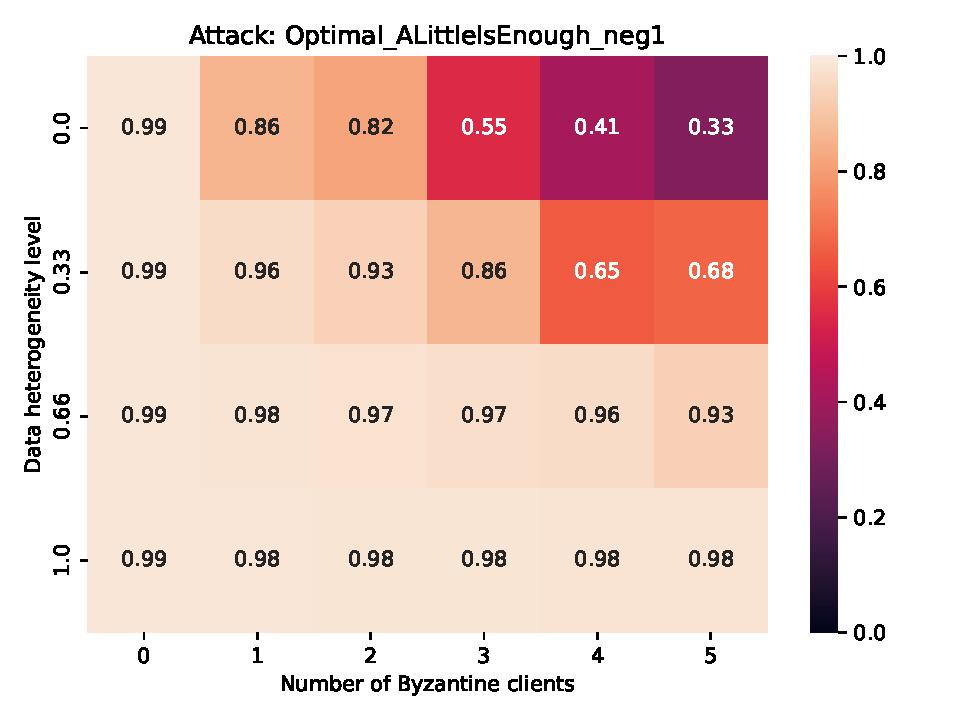
\includegraphics[width=\textwidth]{../plots/cnn_clipped_heatmaps/best_test_Optimal_ALittleIsEnough_neg1_mnist_cnn_mnist_gamma_similarity_niid_NNM_ARC_nb_honest_clients_10_tolerated_f_equal_real.pdf}
        \caption{Grad-Norm Clip $=21$}
        \label{fig:best_alie_gradnorm21}
    \end{subfigure}
    \vspace{0.3cm}
    \begin{subfigure}[b]{0.32\textwidth}
        \centering
        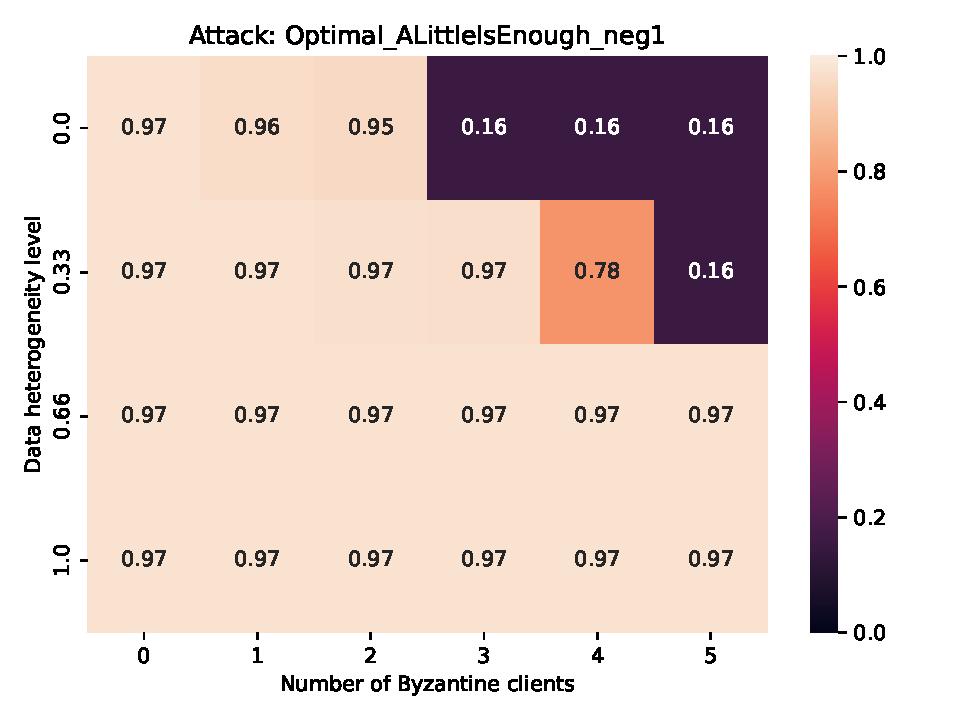
\includegraphics[width=\textwidth]{../plots/mnist_clipping_heatmaps/cnn_mnist_clipping_1/best_test_Optimal_ALittleIsEnough_neg1_mnist_cnn_mnist_clipping_1_gamma_similarity_niid_NNM_ARC_nb_honest_clients_10_tolerated_f_equal_real.pdf}
        \caption{Hardtanh $C{=}1$}
        \label{fig:best_alie_hardtanh_1}
    \end{subfigure}
    \hfill
    \begin{subfigure}[b]{0.32\textwidth}
        \centering
        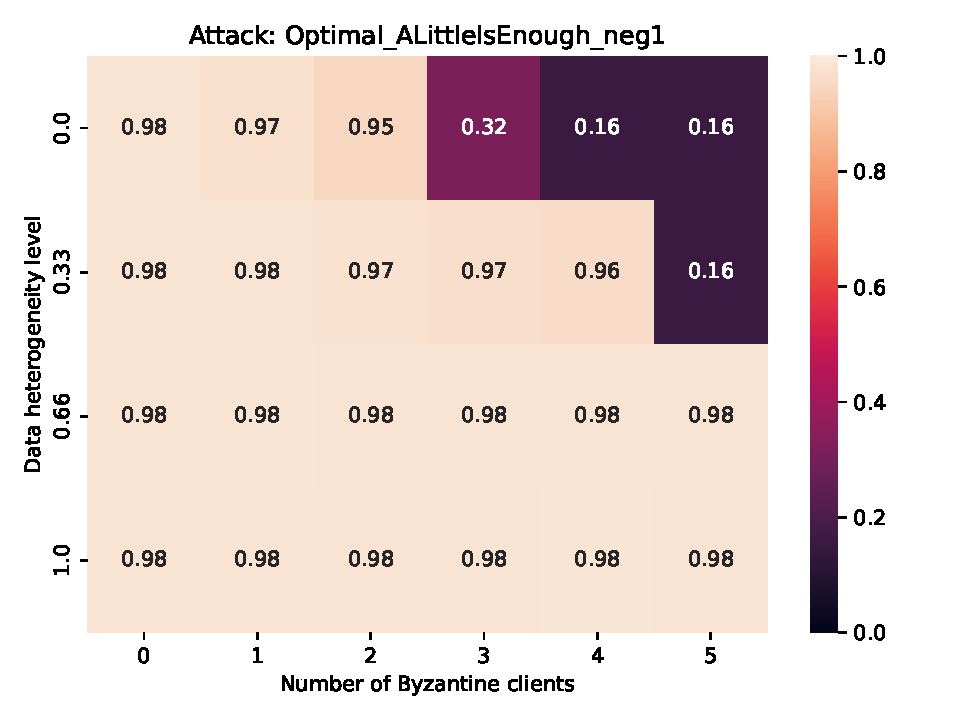
\includegraphics[width=\textwidth]{../plots/mnist_clipping_heatmaps/cnn_mnist_clipping_2/best_test_Optimal_ALittleIsEnough_neg1_mnist_cnn_mnist_clipping_2_gamma_similarity_niid_NNM_ARC_nb_honest_clients_10_tolerated_f_equal_real.pdf}
        \caption{Hardtanh $C{=}2$}
        \label{fig:best_alie_hardtanh_2}
    \end{subfigure}
    \hfill
    \begin{subfigure}[b]{0.32\textwidth}
        \centering
        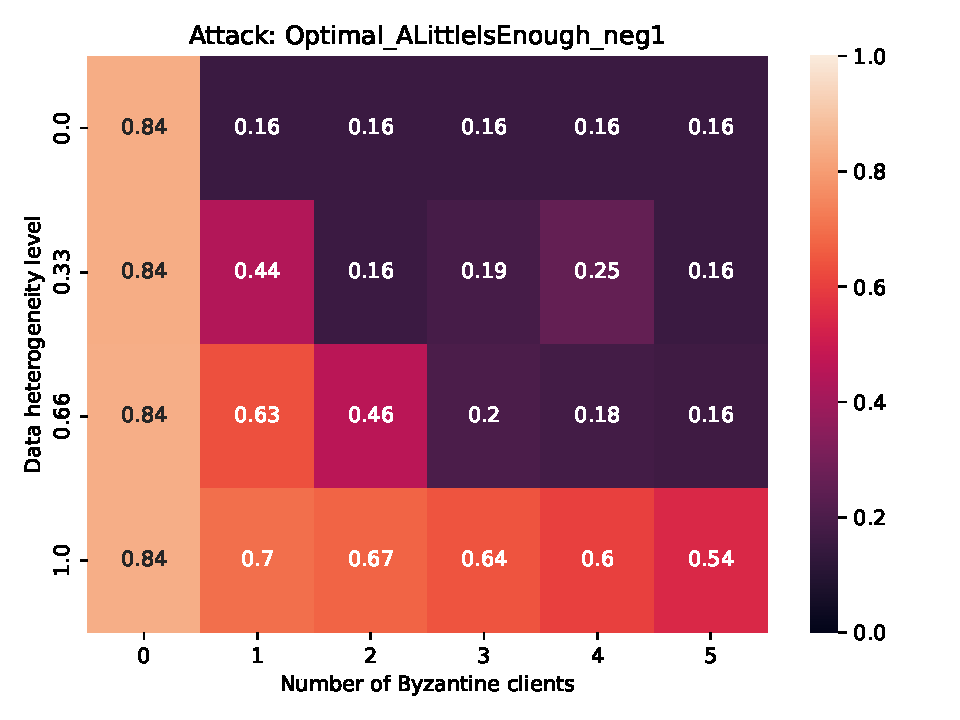
\includegraphics[width=\textwidth]{../activation_clip_plots/cnn_mnist_clip_ste_1/best_test_Optimal_ALittleIsEnough_neg1_mnist_cnn_mnist_clip_ste_1_gamma_similarity_niid_NNM_ARC_nb_honest_clients_10_tolerated_f_equal_real.pdf}
        \caption{STE $C{=}1$}
        \label{fig:best_alie_ste_1}
    \end{subfigure}
    \vspace{0.3cm}
    \begin{subfigure}[b]{0.32\textwidth}
        \centering
        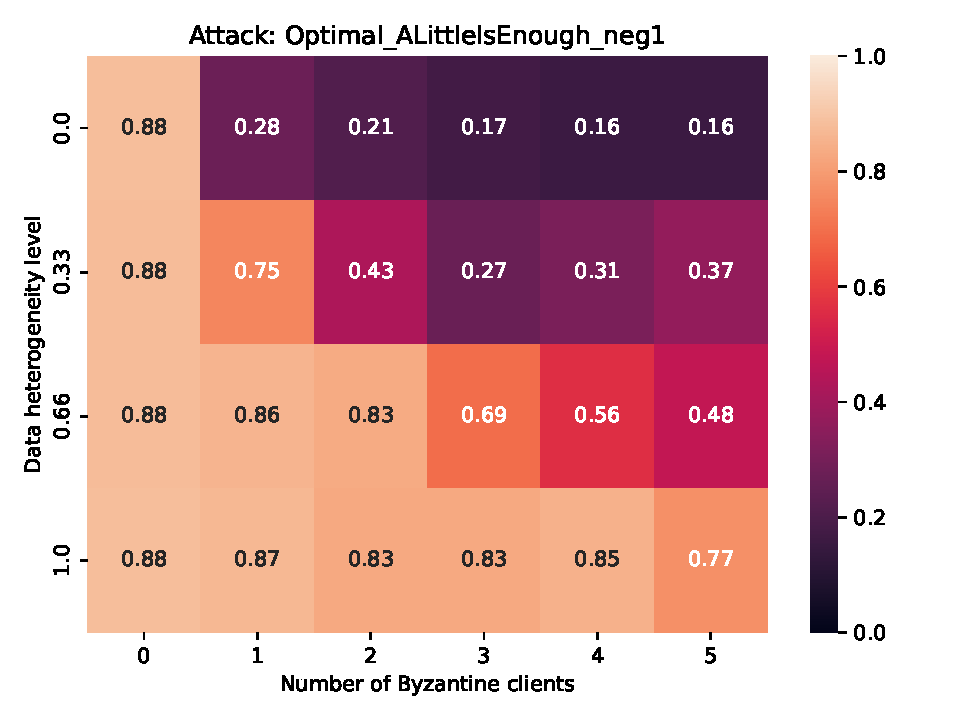
\includegraphics[width=\textwidth]{../activation_clip_plots/cnn_mnist_clip_ste_2/best_test_Optimal_ALittleIsEnough_neg1_mnist_cnn_mnist_clip_ste_2_gamma_similarity_niid_NNM_ARC_nb_honest_clients_10_tolerated_f_equal_real.pdf}
        \caption{STE $C{=}2$}
        \label{fig:best_alie_ste_2}
    \end{subfigure}
    \hfill
    \begin{subfigure}[b]{0.32\textwidth}
        \centering
        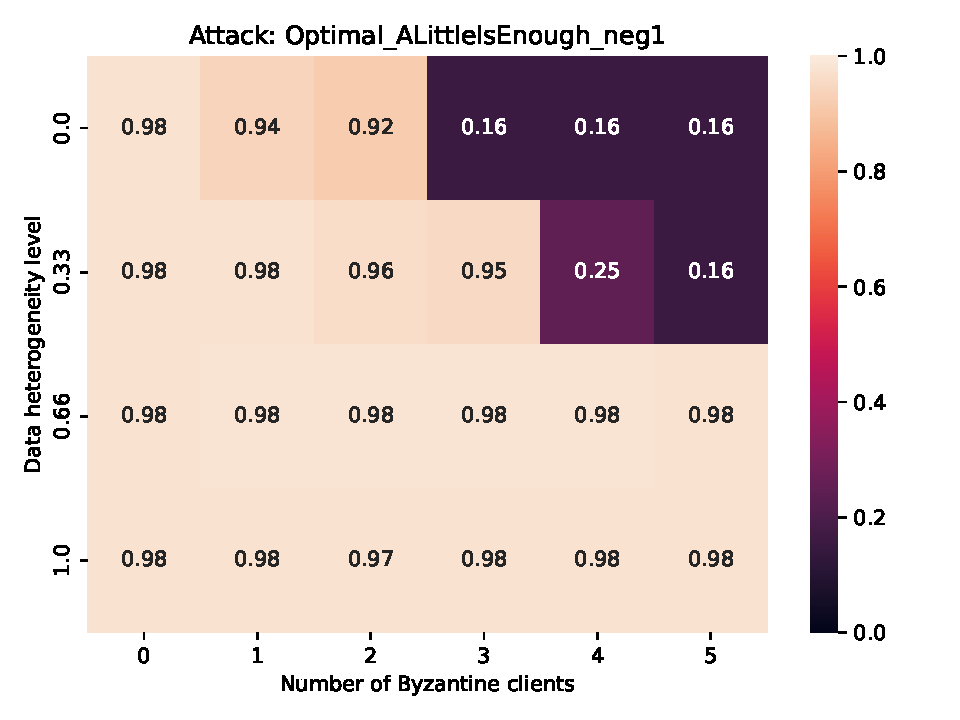
\includegraphics[width=\textwidth]{../activation_clip_plots/cnn_mnist_clip_ramp_1/best_test_Optimal_ALittleIsEnough_neg1_mnist_cnn_mnist_clip_ramp_1_gamma_similarity_niid_NNM_ARC_nb_honest_clients_10_tolerated_f_equal_real.pdf}
        \caption{Ramp $C{=}1$ ($r{=}2$)}
        \label{fig:best_alie_ramp_1}
    \end{subfigure}
    \caption{Best test accuracy under ALIE.}
    \label{fig:best_alie_grid}
\end{figure}
\clearpage
\subsection{Sign Flipping Attack}
\begin{figure}[htbp]
    \centering
    \begin{subfigure}[b]{0.32\textwidth}
        \centering
        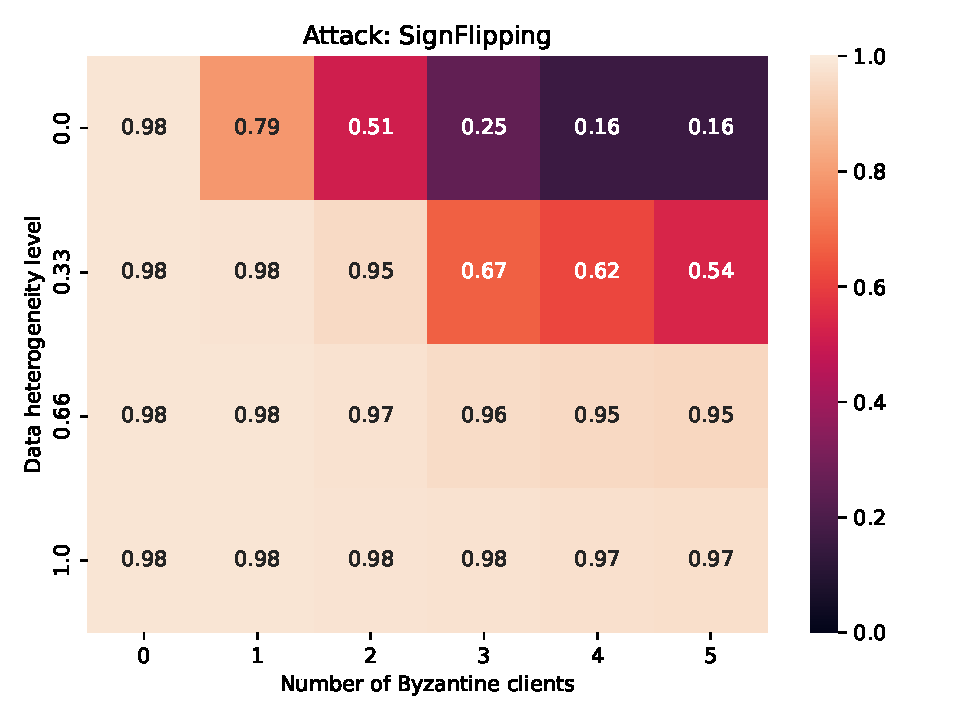
\includegraphics[width=\textwidth]{../plots/mnist_clipping_heatmaps/cnn_mnist/best_test_SignFlipping_mnist_cnn_mnist_gamma_similarity_niid_NNM_ARC_nb_honest_clients_10_tolerated_f_equal_real.pdf}
        \caption{No Clip (ReLU)}
        \label{fig:best_sf_noclip}
    \end{subfigure}
    \hfill
    \begin{subfigure}[b]{0.32\textwidth}
        \centering
        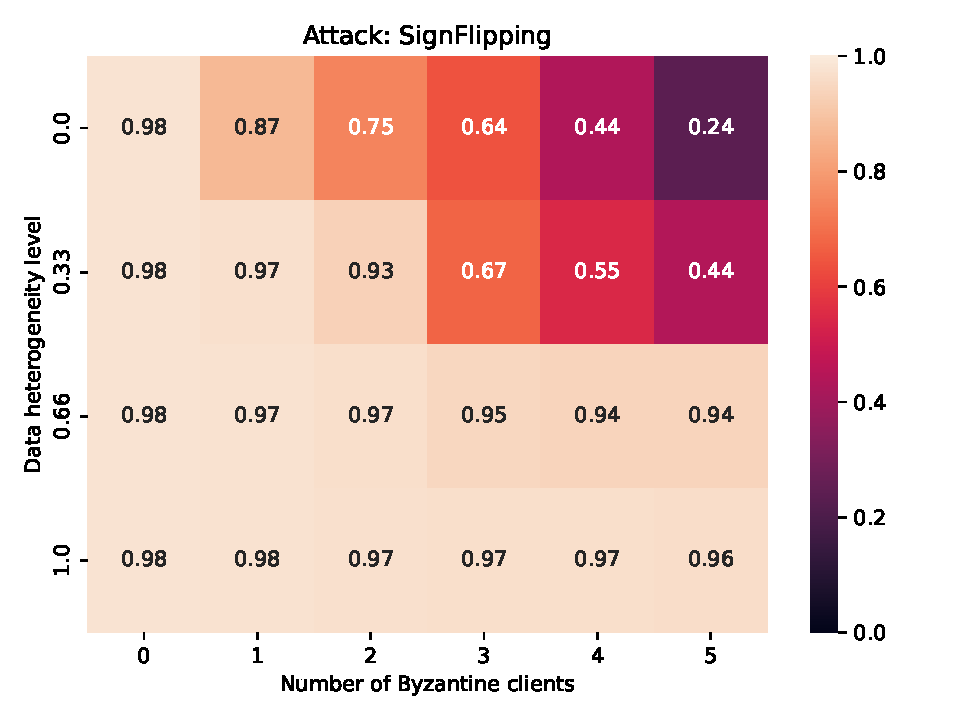
\includegraphics[width=\textwidth]{../plots/cnn_tanh_heatmaps/best_test_SignFlipping_mnist_cnn_mnist_tanh_gamma_similarity_niid_NNM_ARC_nb_honest_clients_10_tolerated_f_equal_real.pdf}
        \caption{Tanh}
        \label{fig:best_sf_tanh}
    \end{subfigure}
    \hfill
    \begin{subfigure}[b]{0.32\textwidth}
        \centering
        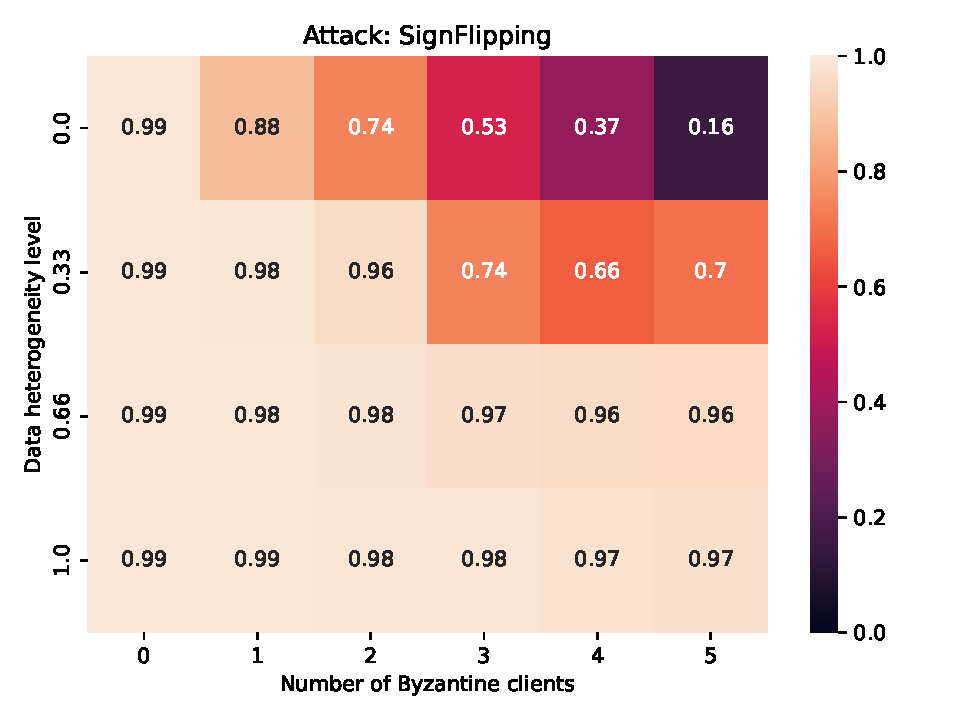
\includegraphics[width=\textwidth]{../plots/cnn_clipped_heatmaps/best_test_SignFlipping_mnist_cnn_mnist_gamma_similarity_niid_NNM_ARC_nb_honest_clients_10_tolerated_f_equal_real.pdf}
        \caption{Grad-Norm Clip $=21$}
        \label{fig:best_sf_gradnorm21}
    \end{subfigure}
    \vspace{0.3cm}
    \begin{subfigure}[b]{0.32\textwidth}
        \centering
        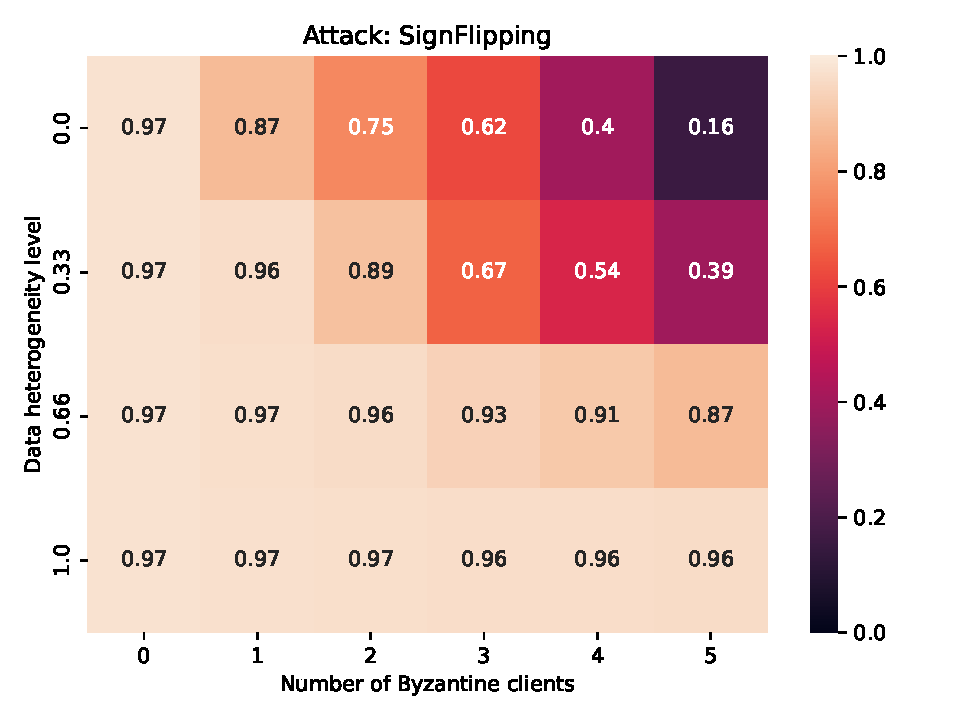
\includegraphics[width=\textwidth]{../plots/mnist_clipping_heatmaps/cnn_mnist_clipping_1/best_test_SignFlipping_mnist_cnn_mnist_clipping_1_gamma_similarity_niid_NNM_ARC_nb_honest_clients_10_tolerated_f_equal_real.pdf}
        \caption{Hardtanh $C{=}1$}
        \label{fig:best_sf_hardtanh_1}
    \end{subfigure}
    \hfill
    \begin{subfigure}[b]{0.32\textwidth}
        \centering
        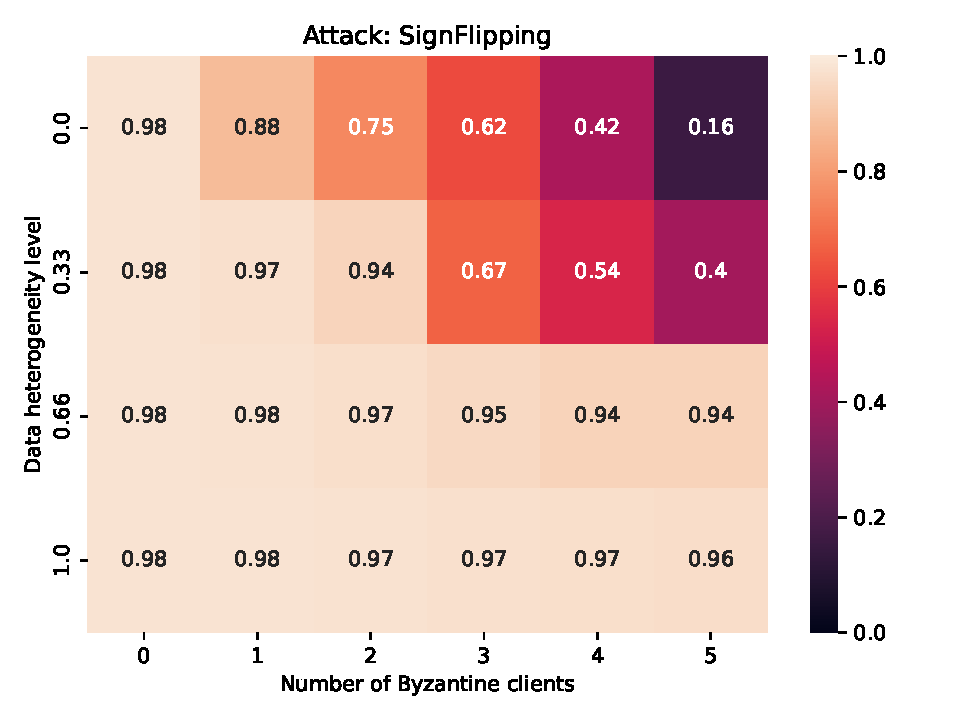
\includegraphics[width=\textwidth]{../plots/mnist_clipping_heatmaps/cnn_mnist_clipping_2/best_test_SignFlipping_mnist_cnn_mnist_clipping_2_gamma_similarity_niid_NNM_ARC_nb_honest_clients_10_tolerated_f_equal_real.pdf}
        \caption{Hardtanh $C{=}2$}
        \label{fig:best_sf_hardtanh_2}
    \end{subfigure}
    \hfill
    \begin{subfigure}[b]{0.32\textwidth}
        \centering
        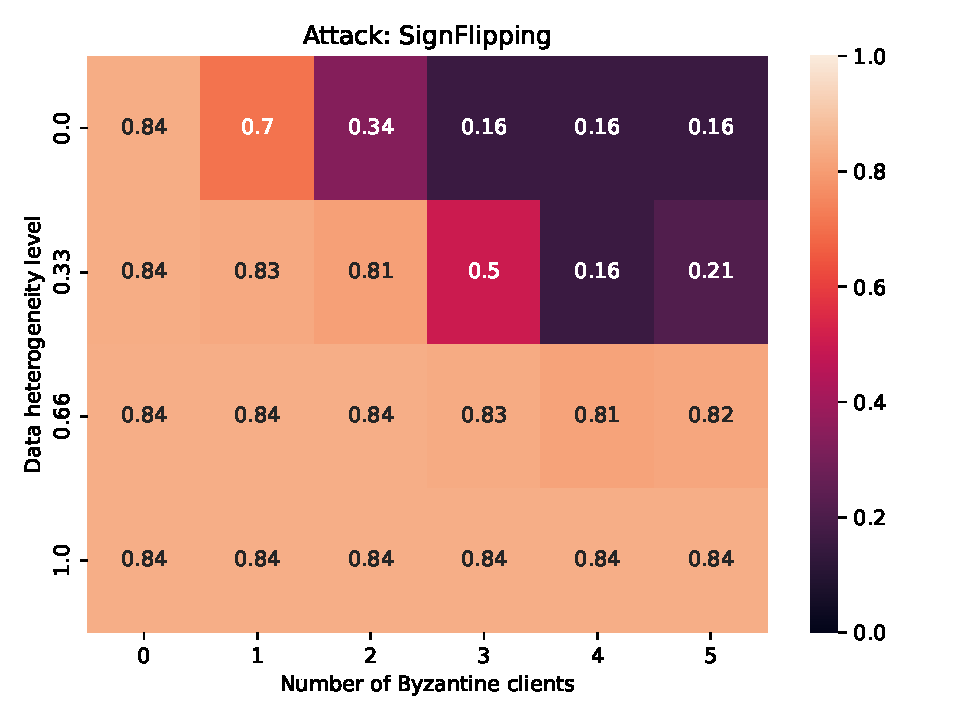
\includegraphics[width=\textwidth]{../activation_clip_plots/cnn_mnist_clip_ste_1/best_test_SignFlipping_mnist_cnn_mnist_clip_ste_1_gamma_similarity_niid_NNM_ARC_nb_honest_clients_10_tolerated_f_equal_real.pdf}
        \caption{STE $C{=}1$}
        \label{fig:best_sf_ste_1}
    \end{subfigure}
    \vspace{0.3cm}
    \begin{subfigure}[b]{0.32\textwidth}
        \centering
        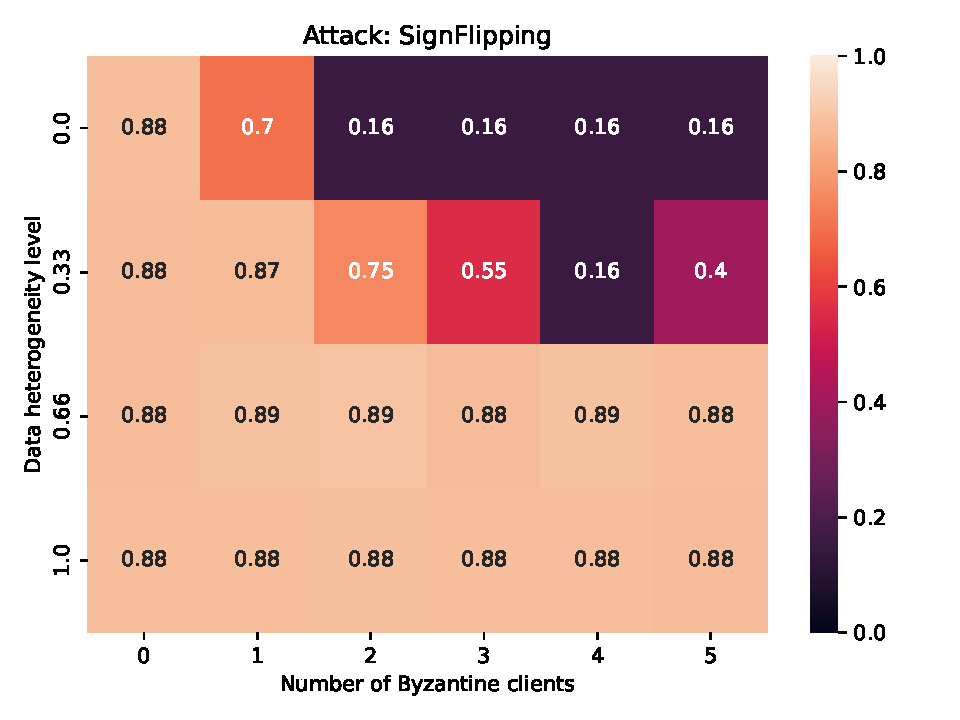
\includegraphics[width=\textwidth]{../activation_clip_plots/cnn_mnist_clip_ste_2/best_test_SignFlipping_mnist_cnn_mnist_clip_ste_2_gamma_similarity_niid_NNM_ARC_nb_honest_clients_10_tolerated_f_equal_real.pdf}
        \caption{STE $C{=}2$}
        \label{fig:best_sf_ste_2}
    \end{subfigure}
    \hfill
    \begin{subfigure}[b]{0.32\textwidth}
        \centering
        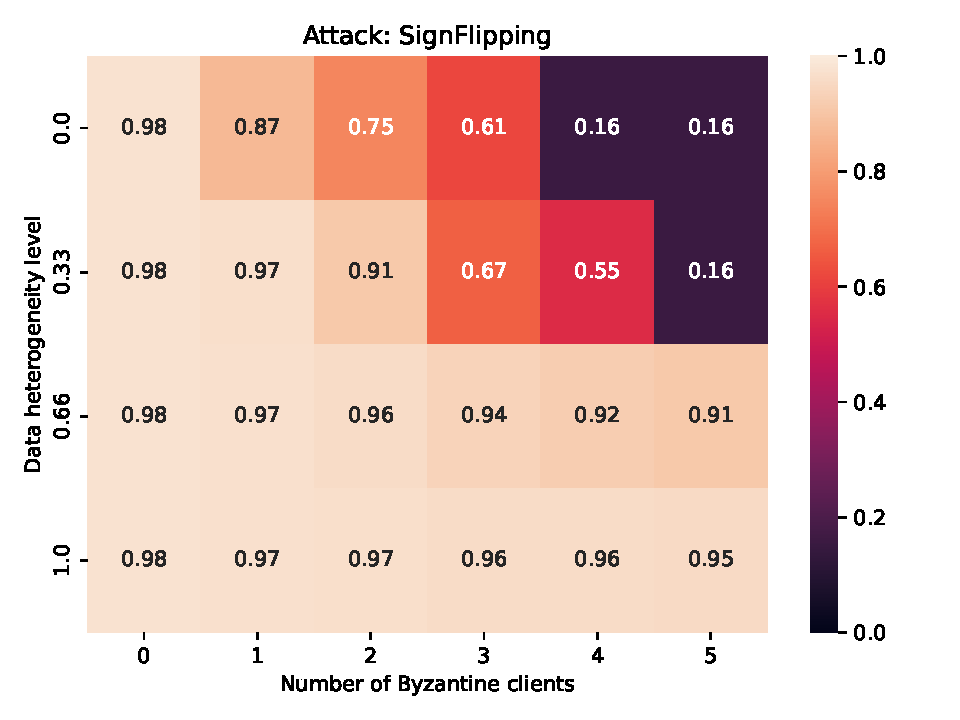
\includegraphics[width=\textwidth]{../activation_clip_plots/cnn_mnist_clip_ramp_1/best_test_SignFlipping_mnist_cnn_mnist_clip_ramp_1_gamma_similarity_niid_NNM_ARC_nb_honest_clients_10_tolerated_f_equal_real.pdf}
        \caption{Ramp $C{=}1$ ($r{=}2$)}
        \label{fig:best_sf_ramp_1}
    \end{subfigure}
    \caption{Best test accuracy under SF.}
    \label{fig:best_sf_grid}
\end{figure}
\clearpage
\subsection{Optimal IPM Attack}
\begin{figure}[htbp]
    \centering
    \begin{subfigure}[b]{0.32\textwidth}
        \centering
        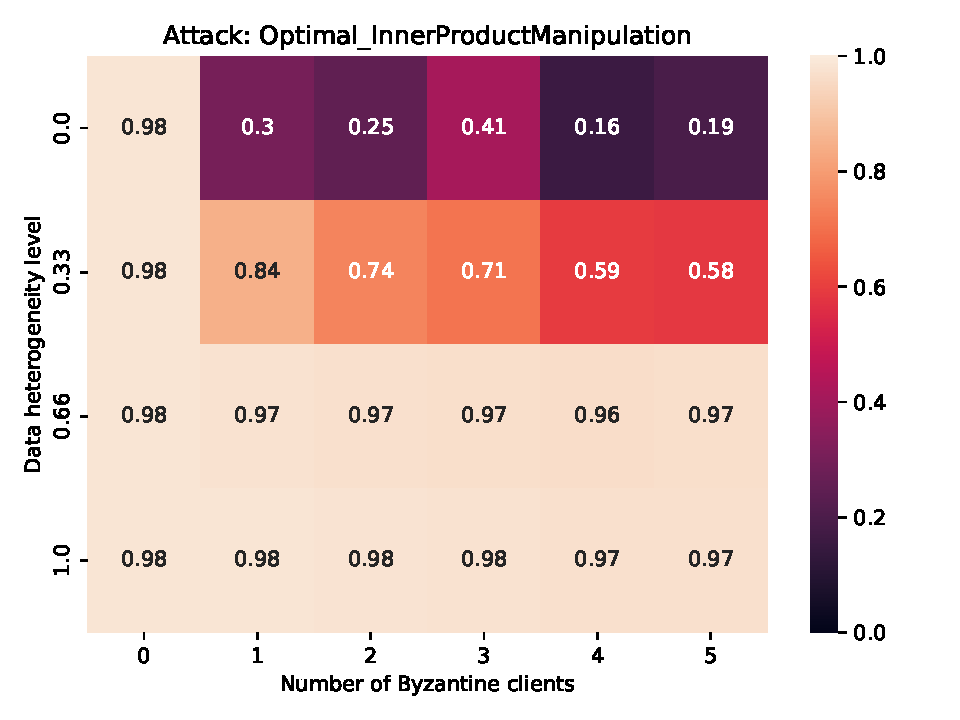
\includegraphics[width=\textwidth]{../plots/mnist_clipping_heatmaps/cnn_mnist/best_test_Optimal_InnerProductManipulation_mnist_cnn_mnist_gamma_similarity_niid_NNM_ARC_nb_honest_clients_10_tolerated_f_equal_real.pdf}
        \caption{No Clip (ReLU)}
        \label{fig:best_ipm_noclip}
    \end{subfigure}
    \hfill
    \begin{subfigure}[b]{0.32\textwidth}
        \centering
        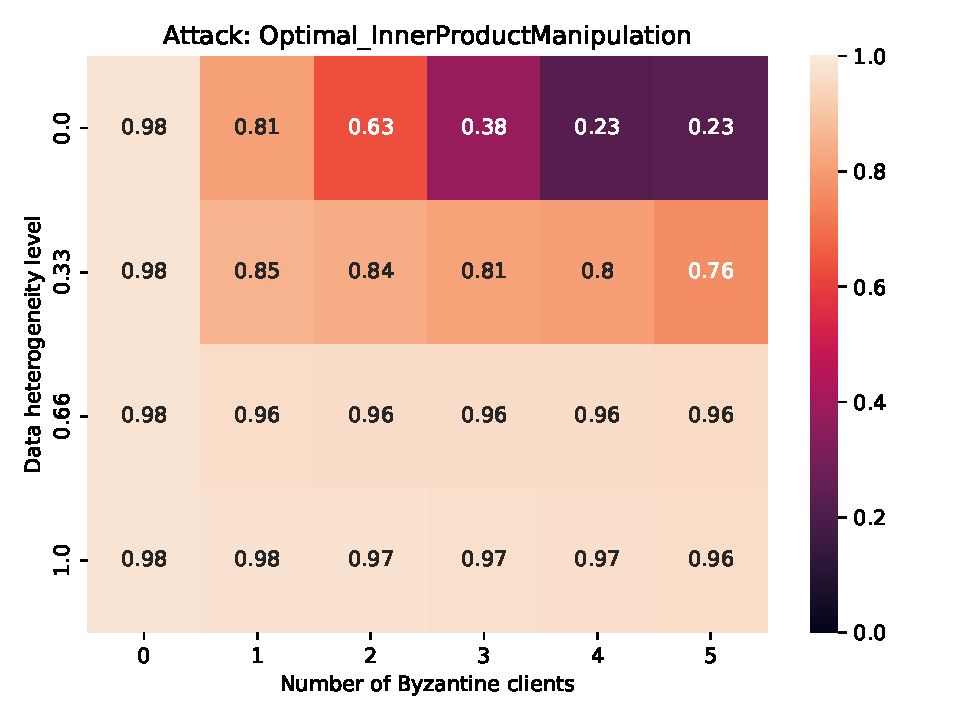
\includegraphics[width=\textwidth]{../plots/cnn_tanh_heatmaps/best_test_Optimal_InnerProductManipulation_mnist_cnn_mnist_tanh_gamma_similarity_niid_NNM_ARC_nb_honest_clients_10_tolerated_f_equal_real.pdf}
        \caption{Tanh}
        \label{fig:best_ipm_tanh}
    \end{subfigure}
    \hfill
    \begin{subfigure}[b]{0.32\textwidth}
        \centering
        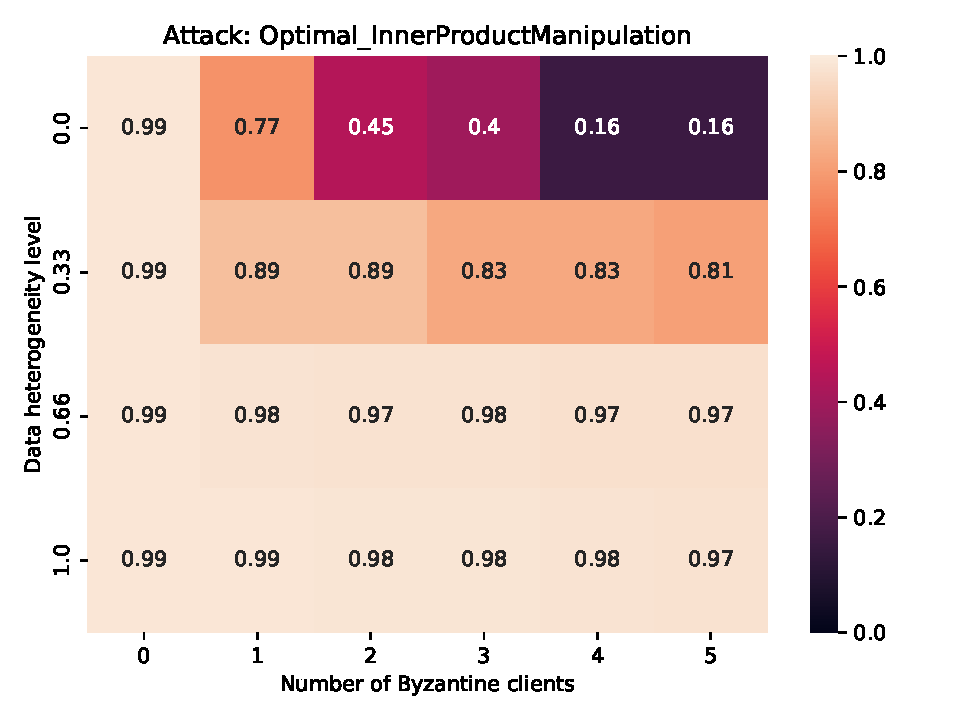
\includegraphics[width=\textwidth]{../plots/cnn_clipped_heatmaps/best_test_Optimal_InnerProductManipulation_mnist_cnn_mnist_gamma_similarity_niid_NNM_ARC_nb_honest_clients_10_tolerated_f_equal_real.pdf}
        \caption{Grad-Norm Clip $=21$}
        \label{fig:best_ipm_gradnorm21}
    \end{subfigure}
    \vspace{0.3cm}
    \begin{subfigure}[b]{0.32\textwidth}
        \centering
        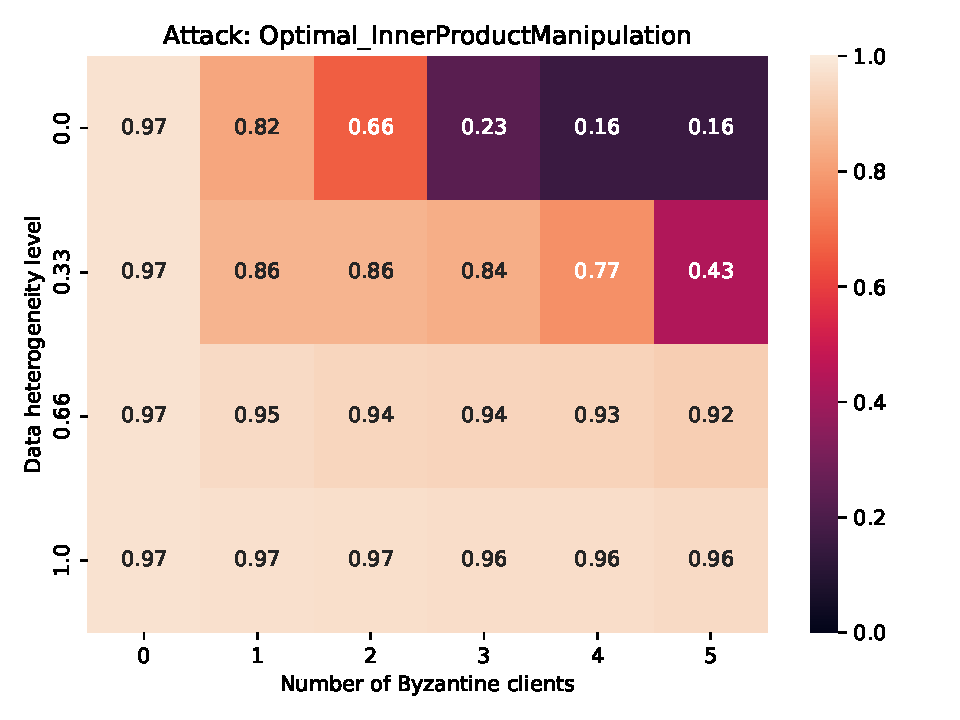
\includegraphics[width=\textwidth]{../plots/mnist_clipping_heatmaps/cnn_mnist_clipping_1/best_test_Optimal_InnerProductManipulation_mnist_cnn_mnist_clipping_1_gamma_similarity_niid_NNM_ARC_nb_honest_clients_10_tolerated_f_equal_real.pdf}
        \caption{Hardtanh $C{=}1$}
        \label{fig:best_ipm_hardtanh_1}
    \end{subfigure}
    \hfill
    \begin{subfigure}[b]{0.32\textwidth}
        \centering
        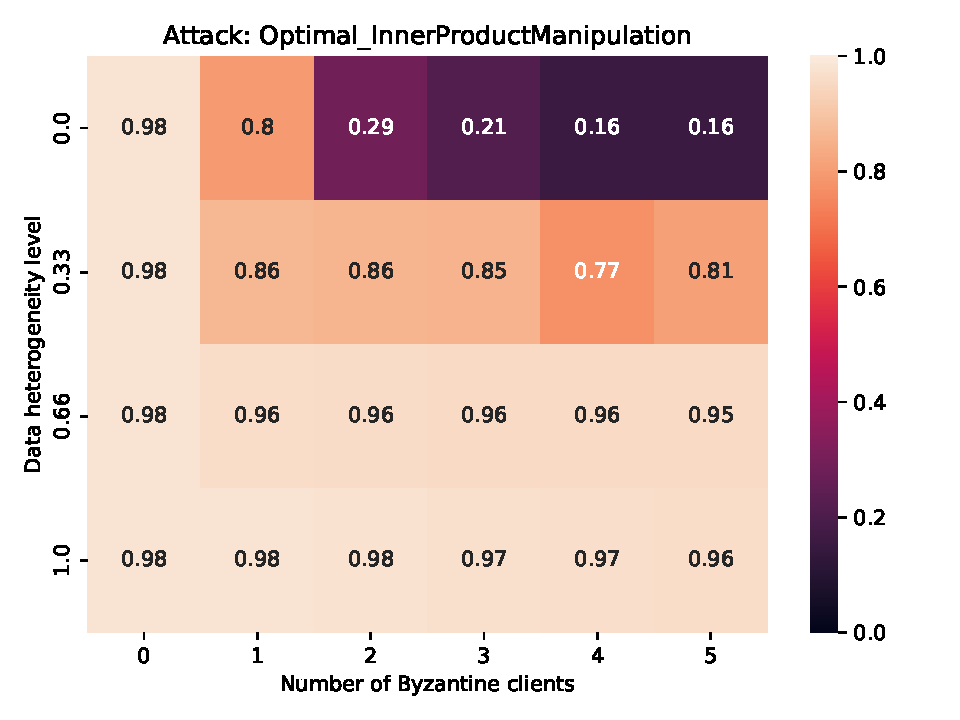
\includegraphics[width=\textwidth]{../plots/mnist_clipping_heatmaps/cnn_mnist_clipping_2/best_test_Optimal_InnerProductManipulation_mnist_cnn_mnist_clipping_2_gamma_similarity_niid_NNM_ARC_nb_honest_clients_10_tolerated_f_equal_real.pdf}
        \caption{Hardtanh $C{=}2$}
        \label{fig:best_ipm_hardtanh_2}
    \end{subfigure}
    \hfill
    \begin{subfigure}[b]{0.32\textwidth}
        \centering
        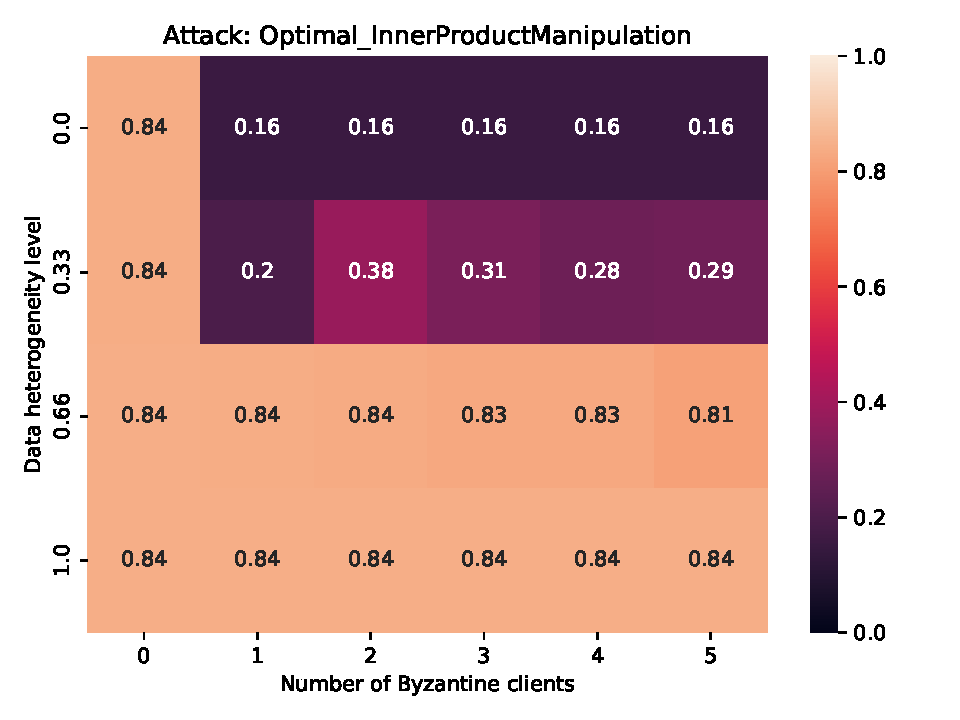
\includegraphics[width=\textwidth]{../activation_clip_plots/cnn_mnist_clip_ste_1/best_test_Optimal_InnerProductManipulation_mnist_cnn_mnist_clip_ste_1_gamma_similarity_niid_NNM_ARC_nb_honest_clients_10_tolerated_f_equal_real.pdf}
        \caption{STE $C{=}1$}
        \label{fig:best_ipm_ste_1}
    \end{subfigure}
    \vspace{0.3cm}
    \begin{subfigure}[b]{0.32\textwidth}
        \centering
        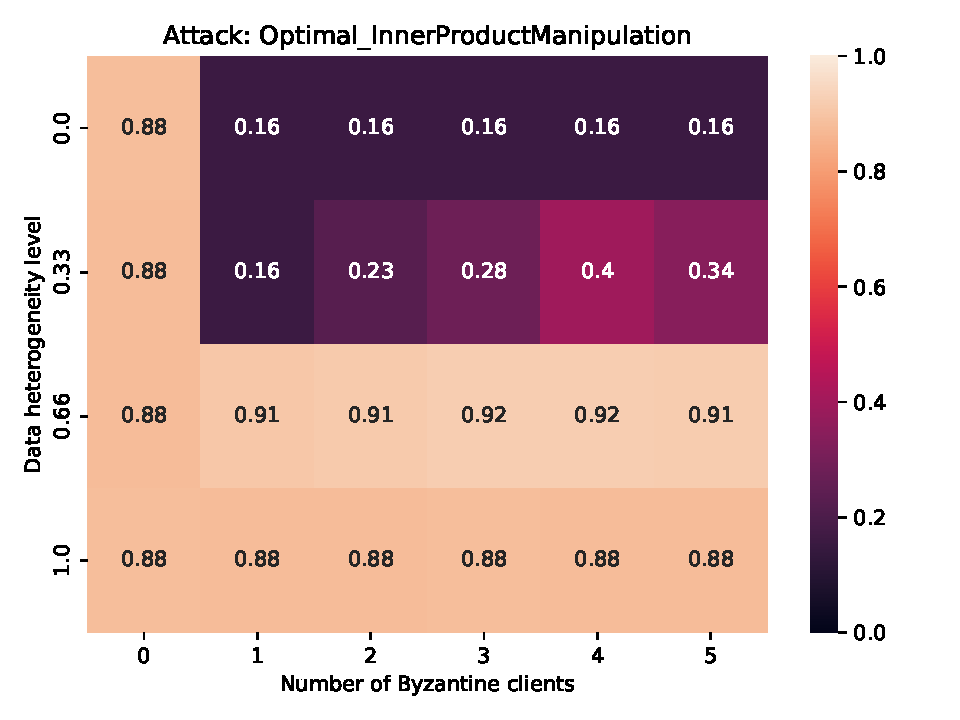
\includegraphics[width=\textwidth]{../activation_clip_plots/cnn_mnist_clip_ste_2/best_test_Optimal_InnerProductManipulation_mnist_cnn_mnist_clip_ste_2_gamma_similarity_niid_NNM_ARC_nb_honest_clients_10_tolerated_f_equal_real.pdf}
        \caption{STE $C{=}2$}
        \label{fig:best_ipm_ste_2}
    \end{subfigure}
    \hfill
    \begin{subfigure}[b]{0.32\textwidth}
        \centering
        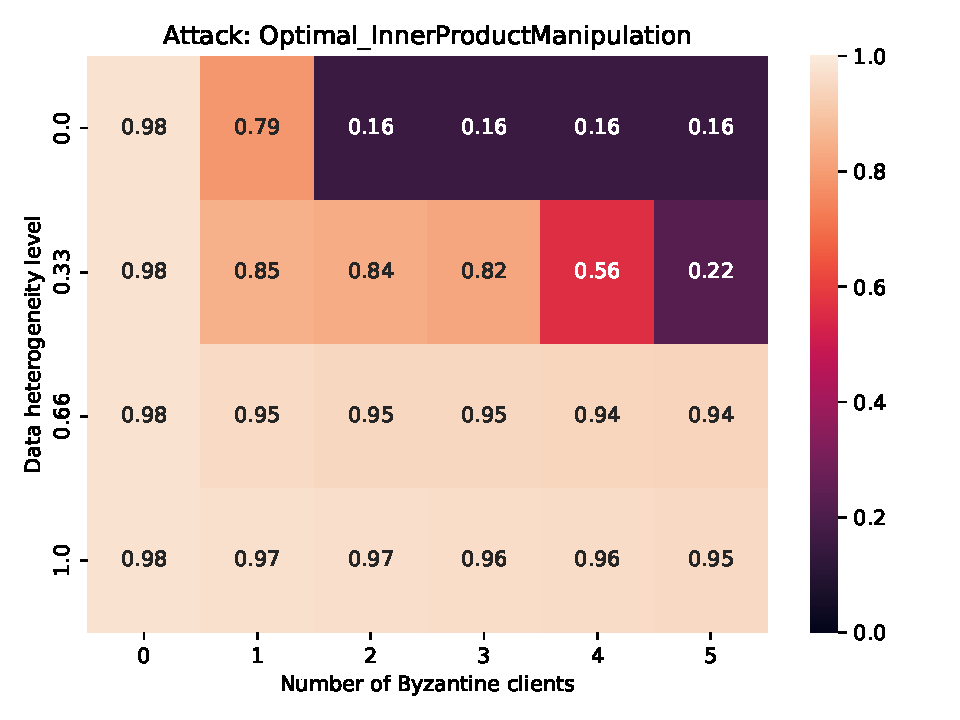
\includegraphics[width=\textwidth]{../activation_clip_plots/cnn_mnist_clip_ramp_1/best_test_Optimal_InnerProductManipulation_mnist_cnn_mnist_clip_ramp_1_gamma_similarity_niid_NNM_ARC_nb_honest_clients_10_tolerated_f_equal_real.pdf}
        \caption{Ramp $C{=}1$ ($r{=}2$)}
        \label{fig:best_ipm_ramp_1}
    \end{subfigure}
    \caption{Best test accuracy under IPM.}
    \label{fig:best_ipm_grid}
\end{figure}
\clearpage
\section{Centered Clipping (CC)}
\subsection{CC under Worst-Case across all Attacks}
\begin{figure}[htbp]
    \centering
    \begin{subfigure}[b]{0.32\textwidth}
        \centering
        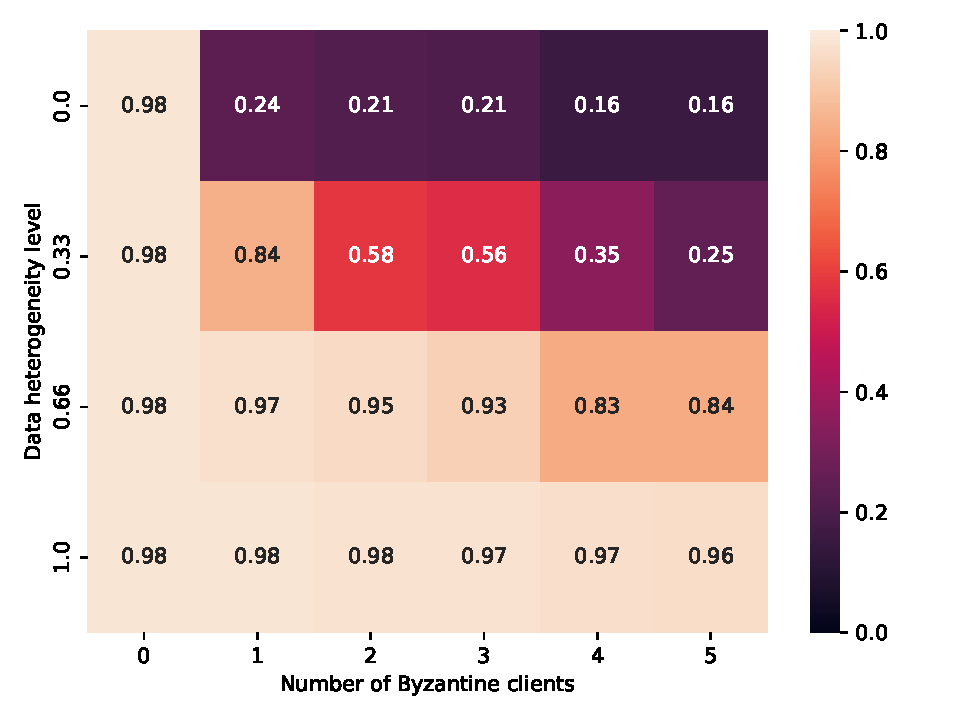
\includegraphics[width=\textwidth]{../plots/mnist_clipping_heatmaps/cnn_mnist/test_mnist_cnn_mnist_gamma_similarity_niid_NNM_ARC_CenteredClipping_nb_honest_clients_10_tolerated_f_equal_real.pdf}
        \caption{No Clip (ReLU)}
        \label{fig:cc_worst_case_noclip}
    \end{subfigure}
    \hfill
    \begin{subfigure}[b]{0.32\textwidth}
        \centering
        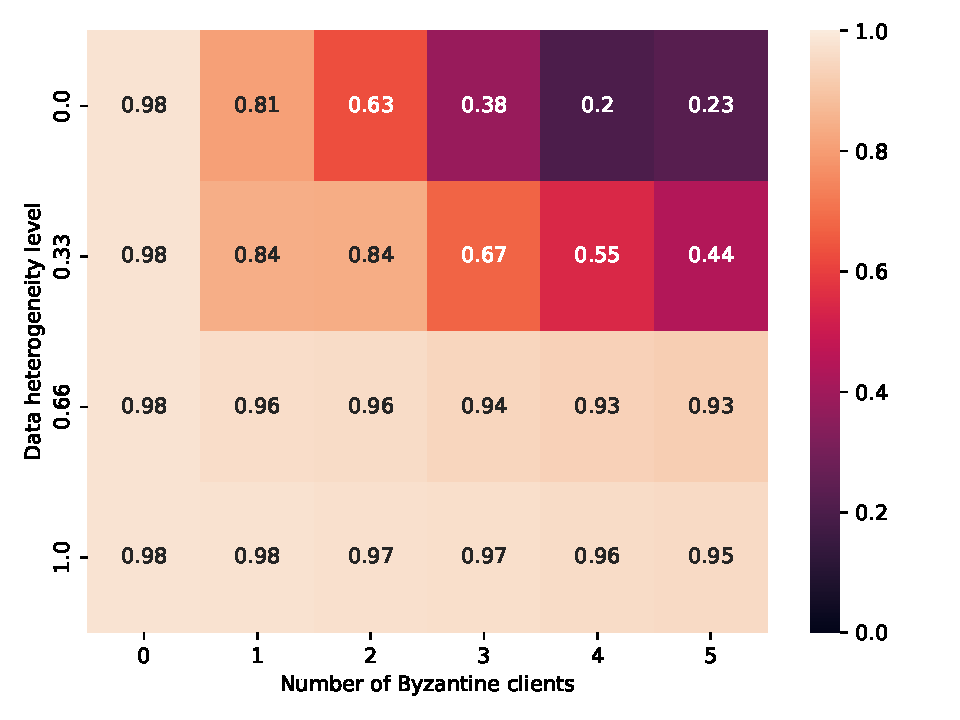
\includegraphics[width=\textwidth]{../plots/cnn_tanh_heatmaps/test_mnist_cnn_mnist_tanh_gamma_similarity_niid_NNM_ARC_CenteredClipping_nb_honest_clients_10_tolerated_f_equal_real.pdf}
        \caption{Tanh}
        \label{fig:cc_worst_case_tanh}
    \end{subfigure}
    \hfill
    \begin{subfigure}[b]{0.32\textwidth}
        \centering
        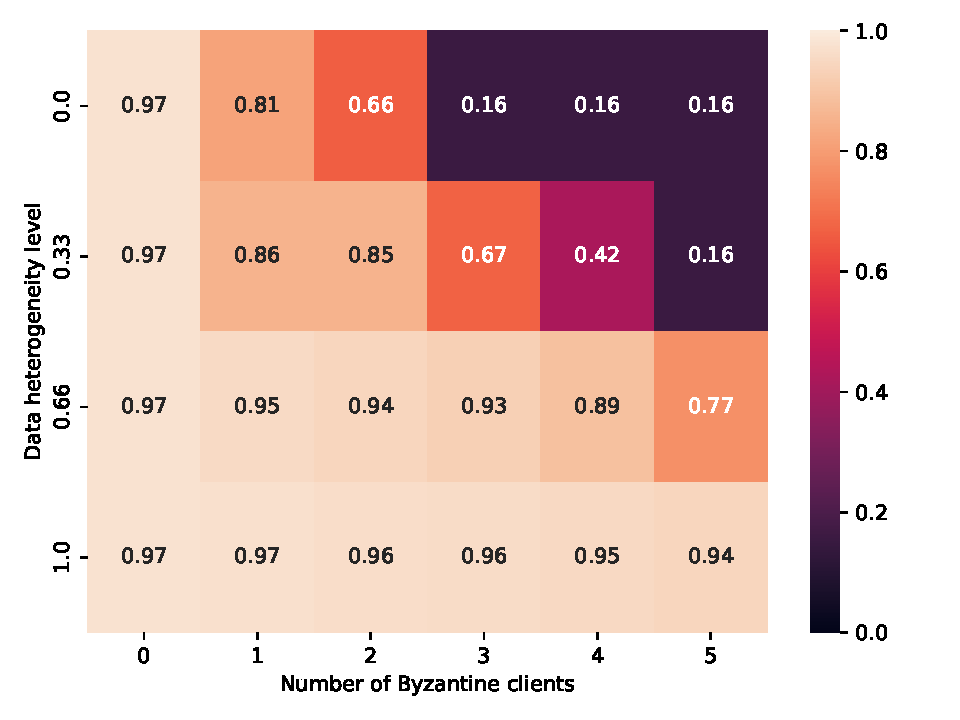
\includegraphics[width=\textwidth]{../plots/mnist_clipping_heatmaps/cnn_mnist_clipping_1/test_mnist_cnn_mnist_clipping_1_gamma_similarity_niid_NNM_ARC_CenteredClipping_nb_honest_clients_10_tolerated_f_equal_real.pdf}
        \caption{Hardtanh $C{=}1$}
        \label{fig:cc_worst_case_hardtanh_1}
    \end{subfigure}
    \vspace{0.3cm}
    \begin{subfigure}[b]{0.32\textwidth}
        \centering
        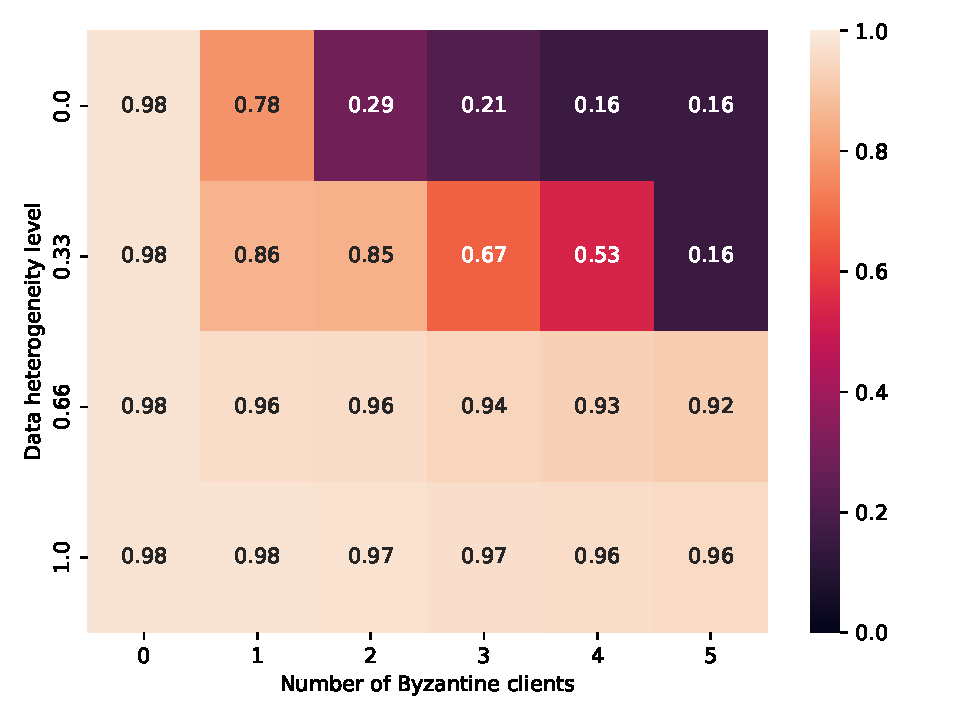
\includegraphics[width=\textwidth]{../plots/mnist_clipping_heatmaps/cnn_mnist_clipping_2/test_mnist_cnn_mnist_clipping_2_gamma_similarity_niid_NNM_ARC_CenteredClipping_nb_honest_clients_10_tolerated_f_equal_real.pdf}
        \caption{Hardtanh $C{=}2$}
        \label{fig:cc_worst_case_hardtanh_2}
    \end{subfigure}
    \hfill
    \begin{subfigure}[b]{0.32\textwidth}
        \centering
        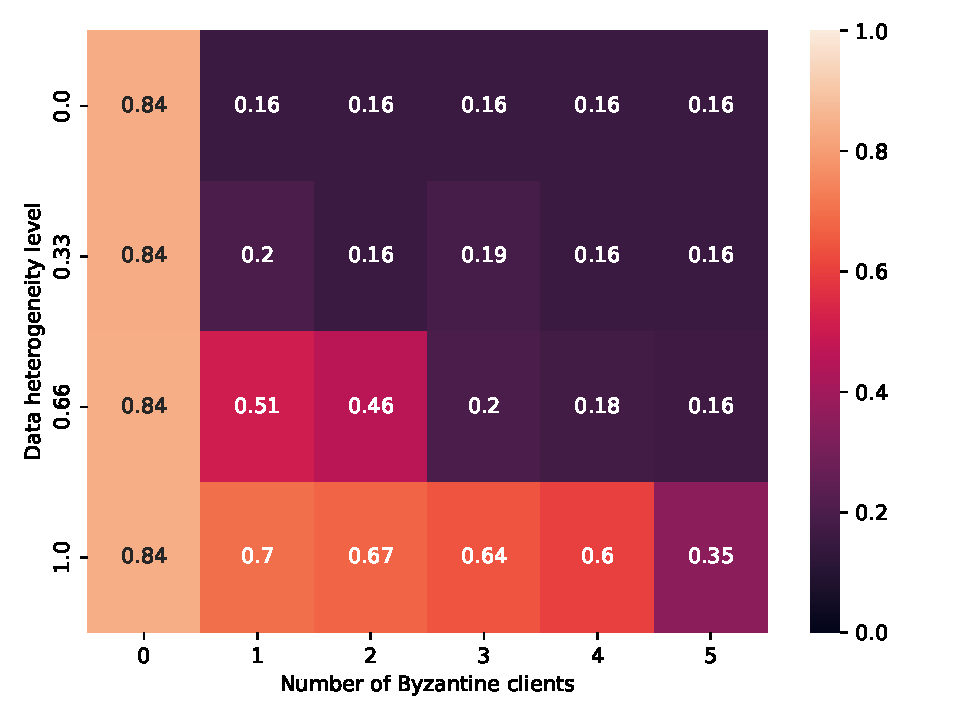
\includegraphics[width=\textwidth]{../activation_clip_plots/cnn_mnist_clip_ste_1/test_mnist_cnn_mnist_clip_ste_1_gamma_similarity_niid_NNM_ARC_CenteredClipping_nb_honest_clients_10_tolerated_f_equal_real.pdf}
        \caption{STE $C{=}1$}
        \label{fig:cc_worst_case_ste_1}
    \end{subfigure}
    \hfill
    \begin{subfigure}[b]{0.32\textwidth}
        \centering
        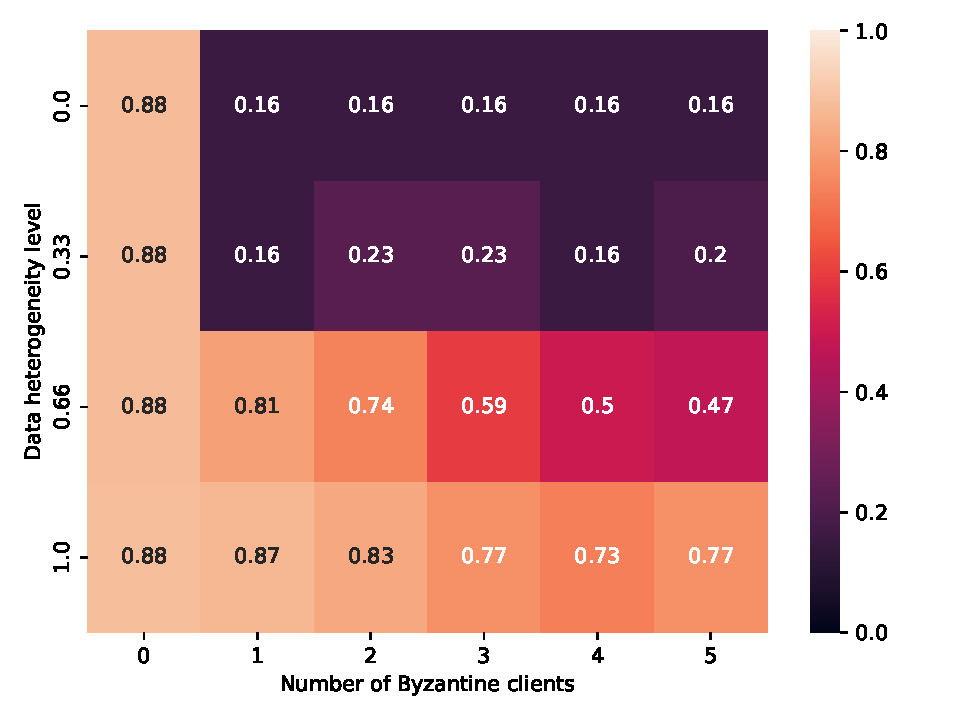
\includegraphics[width=\textwidth]{../activation_clip_plots/cnn_mnist_clip_ste_2/test_mnist_cnn_mnist_clip_ste_2_gamma_similarity_niid_NNM_ARC_CenteredClipping_nb_honest_clients_10_tolerated_f_equal_real.pdf}
        \caption{STE $C{=}2$}
        \label{fig:cc_worst_case_ste_2}
    \end{subfigure}
    \vspace{0.3cm}
    \begin{subfigure}[b]{0.32\textwidth}
        \centering
        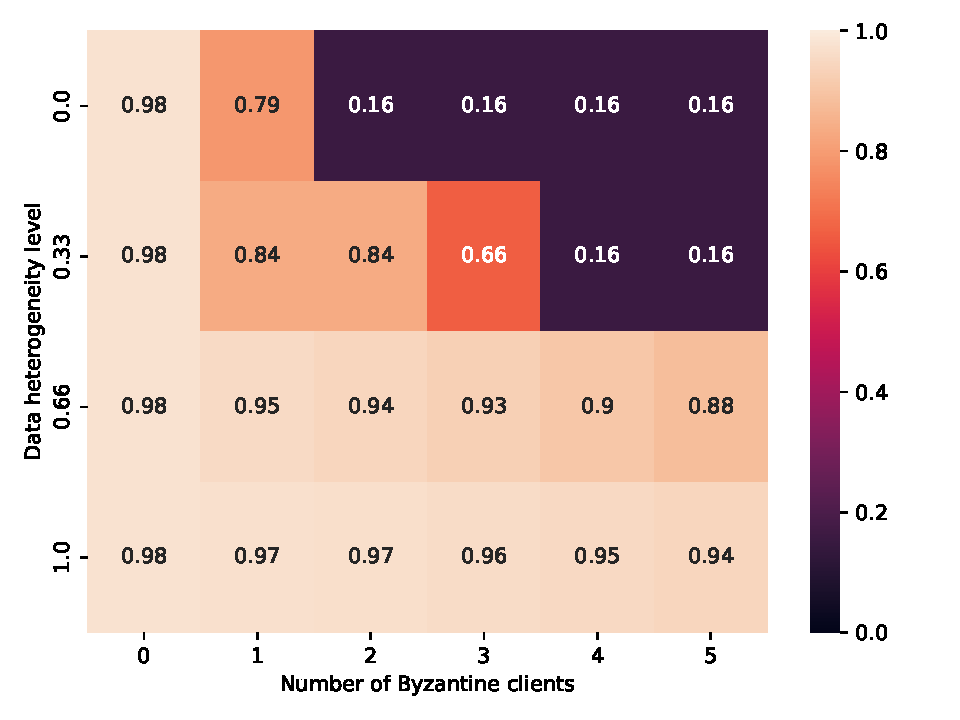
\includegraphics[width=\textwidth]{../activation_clip_plots/cnn_mnist_clip_ramp_1/test_mnist_cnn_mnist_clip_ramp_1_gamma_similarity_niid_NNM_ARC_CenteredClipping_nb_honest_clients_10_tolerated_f_equal_real.pdf}
        \caption{Ramp $C{=}1$ ($r{=}2$)}
        \label{fig:cc_worst_case_ramp_1}
    \end{subfigure}
    \caption{Centered Clipping (CC) under Worst-Case across all Attacks.}
    \label{fig:cc_worst_case_grid}
\end{figure}
\clearpage
\subsection{CC under ALIE}
\begin{figure}[htbp]
    \centering
    \begin{subfigure}[b]{0.32\textwidth}
        \centering
        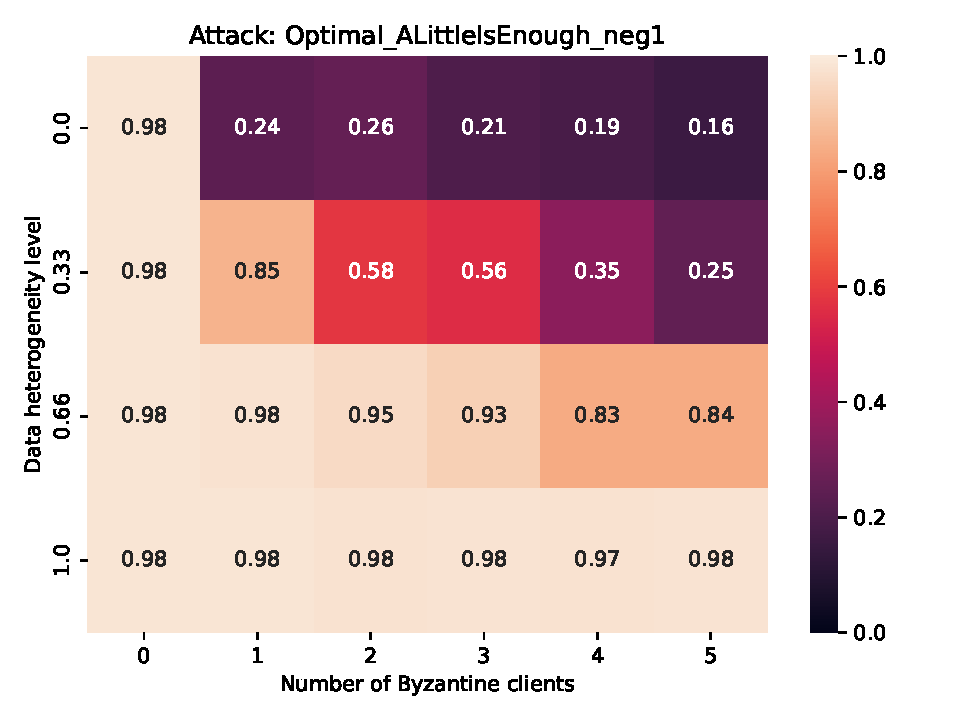
\includegraphics[width=\textwidth]{../plots/mnist_clipping_heatmaps/cnn_mnist/test_Optimal_ALittleIsEnough_neg1_mnist_cnn_mnist_gamma_similarity_niid_NNM_ARC_CenteredClipping_nb_honest_clients_10_tolerated_f_equal_real.pdf}
        \caption{No Clip (ReLU)}
        \label{fig:cc_alie_noclip}
    \end{subfigure}
    \hfill
    \begin{subfigure}[b]{0.32\textwidth}
        \centering
        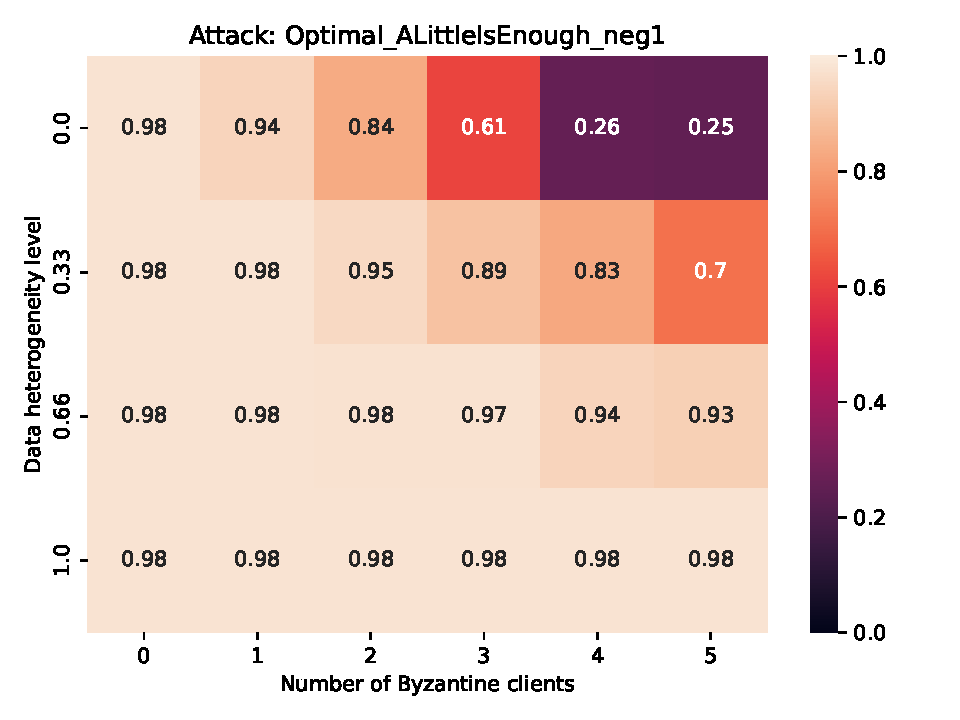
\includegraphics[width=\textwidth]{../plots/cnn_tanh_heatmaps/test_Optimal_ALittleIsEnough_neg1_mnist_cnn_mnist_tanh_gamma_similarity_niid_NNM_ARC_CenteredClipping_nb_honest_clients_10_tolerated_f_equal_real.pdf}
        \caption{Tanh}
        \label{fig:cc_alie_tanh}
    \end{subfigure}
    \hfill
    \begin{subfigure}[b]{0.32\textwidth}
        \centering
        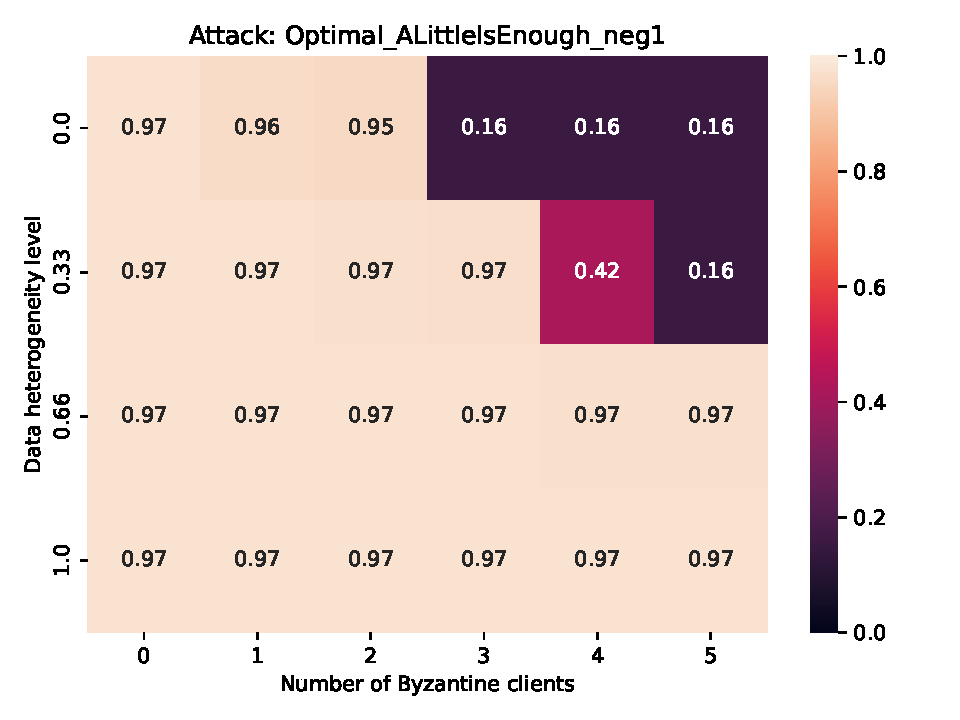
\includegraphics[width=\textwidth]{../plots/mnist_clipping_heatmaps/cnn_mnist_clipping_1/test_Optimal_ALittleIsEnough_neg1_mnist_cnn_mnist_clipping_1_gamma_similarity_niid_NNM_ARC_CenteredClipping_nb_honest_clients_10_tolerated_f_equal_real.pdf}
        \caption{Hardtanh $C{=}1$}
        \label{fig:cc_alie_hardtanh_1}
    \end{subfigure}
    \vspace{0.3cm}
    \begin{subfigure}[b]{0.32\textwidth}
        \centering
        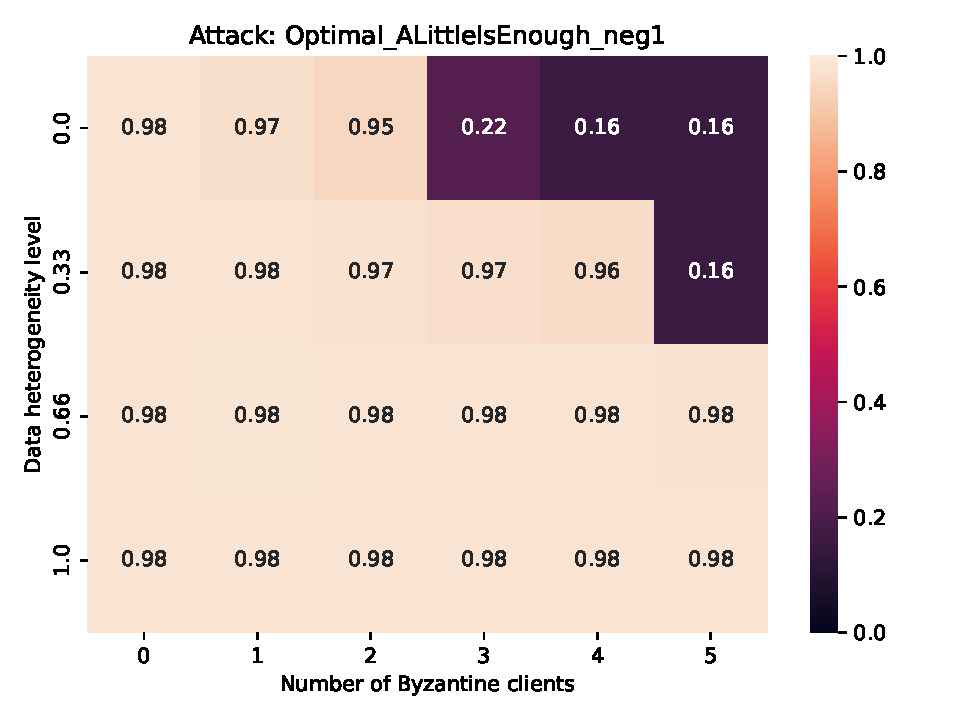
\includegraphics[width=\textwidth]{../plots/mnist_clipping_heatmaps/cnn_mnist_clipping_2/test_Optimal_ALittleIsEnough_neg1_mnist_cnn_mnist_clipping_2_gamma_similarity_niid_NNM_ARC_CenteredClipping_nb_honest_clients_10_tolerated_f_equal_real.pdf}
        \caption{Hardtanh $C{=}2$}
        \label{fig:cc_alie_hardtanh_2}
    \end{subfigure}
    \hfill
    \begin{subfigure}[b]{0.32\textwidth}
        \centering
        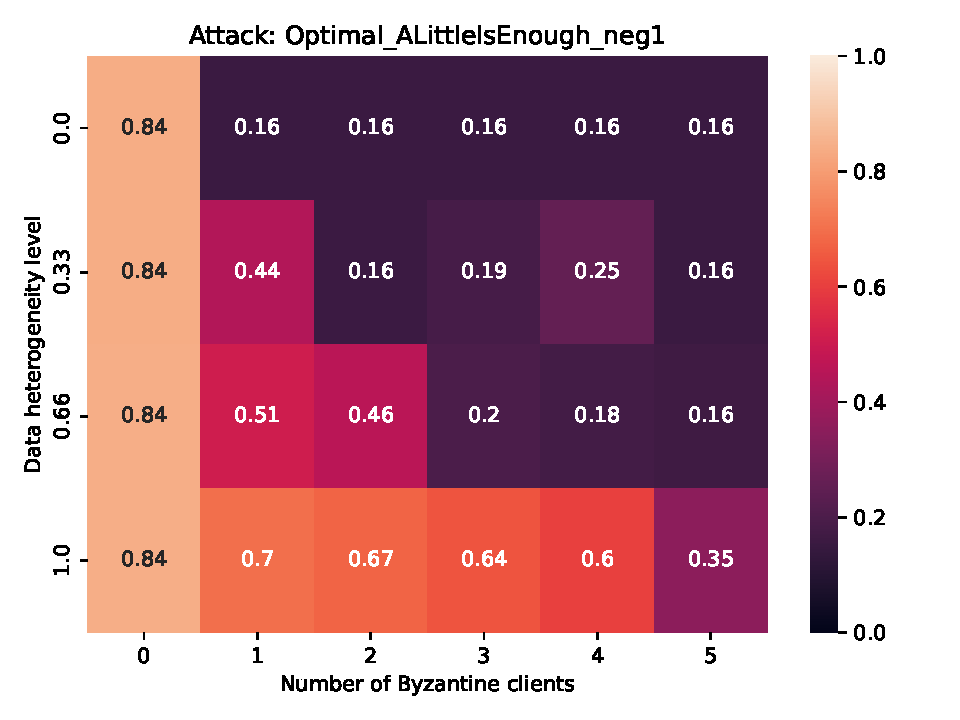
\includegraphics[width=\textwidth]{../activation_clip_plots/cnn_mnist_clip_ste_1/test_Optimal_ALittleIsEnough_neg1_mnist_cnn_mnist_clip_ste_1_gamma_similarity_niid_NNM_ARC_CenteredClipping_nb_honest_clients_10_tolerated_f_equal_real.pdf}
        \caption{STE $C{=}1$}
        \label{fig:cc_alie_ste_1}
    \end{subfigure}
    \hfill
    \begin{subfigure}[b]{0.32\textwidth}
        \centering
        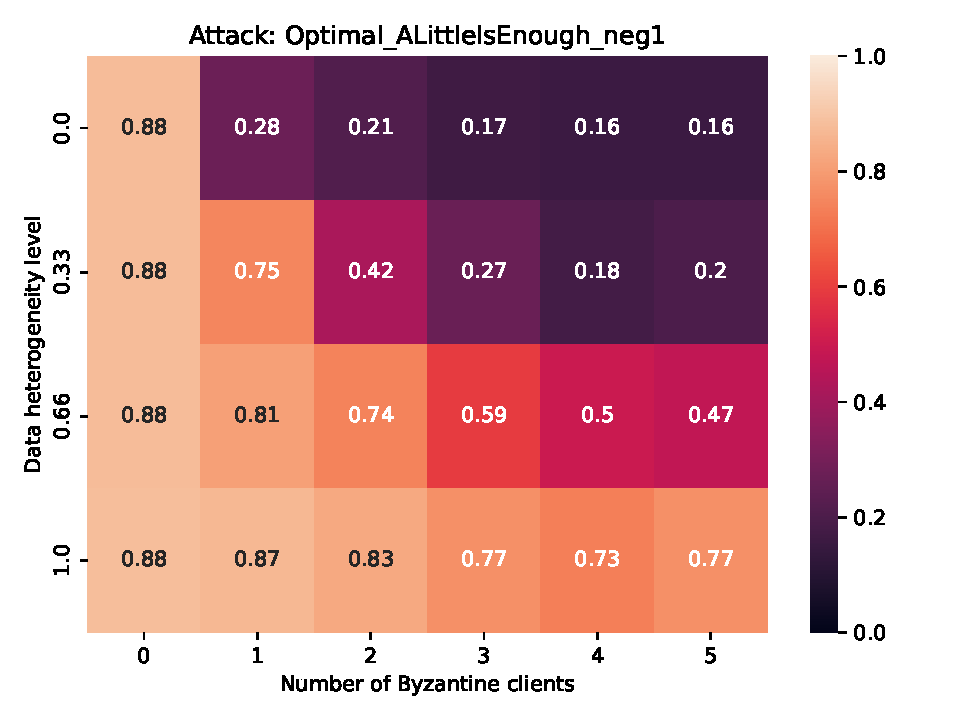
\includegraphics[width=\textwidth]{../activation_clip_plots/cnn_mnist_clip_ste_2/test_Optimal_ALittleIsEnough_neg1_mnist_cnn_mnist_clip_ste_2_gamma_similarity_niid_NNM_ARC_CenteredClipping_nb_honest_clients_10_tolerated_f_equal_real.pdf}
        \caption{STE $C{=}2$}
        \label{fig:cc_alie_ste_2}
    \end{subfigure}
    \vspace{0.3cm}
    \begin{subfigure}[b]{0.32\textwidth}
        \centering
        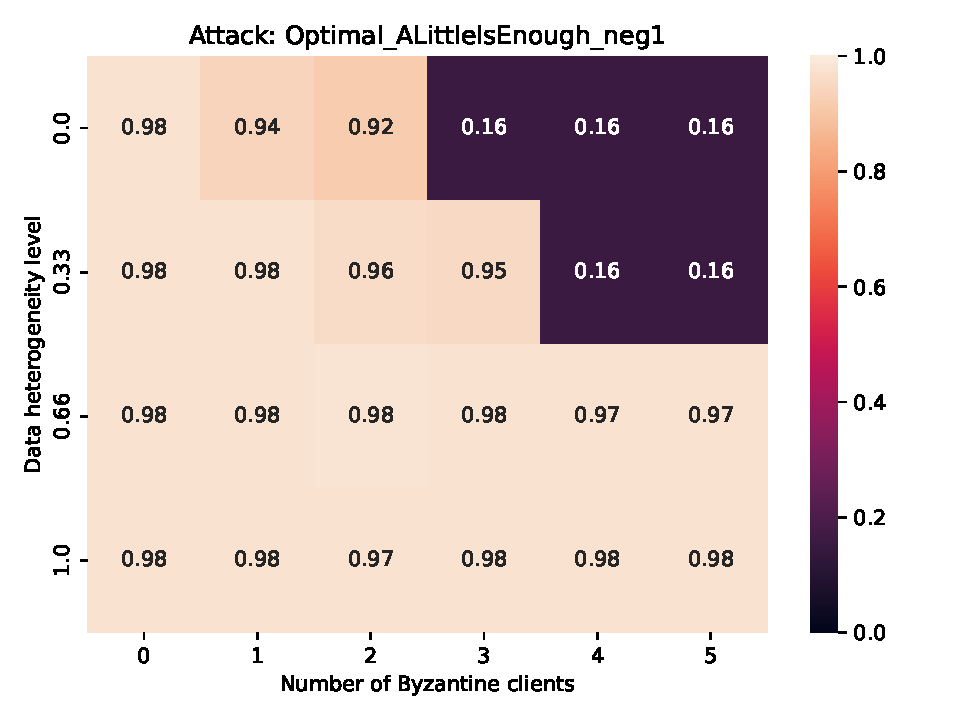
\includegraphics[width=\textwidth]{../activation_clip_plots/cnn_mnist_clip_ramp_1/test_Optimal_ALittleIsEnough_neg1_mnist_cnn_mnist_clip_ramp_1_gamma_similarity_niid_NNM_ARC_CenteredClipping_nb_honest_clients_10_tolerated_f_equal_real.pdf}
        \caption{Ramp $C{=}1$ ($r{=}2$)}
        \label{fig:cc_alie_ramp_1}
    \end{subfigure}
    \caption{Centered Clipping (CC) under Optimal ALIE Attack.}
    \label{fig:cc_alie_grid}
\end{figure}
\clearpage
\subsection{CC under SF}
\begin{figure}[htbp]
    \centering
    \begin{subfigure}[b]{0.32\textwidth}
        \centering
        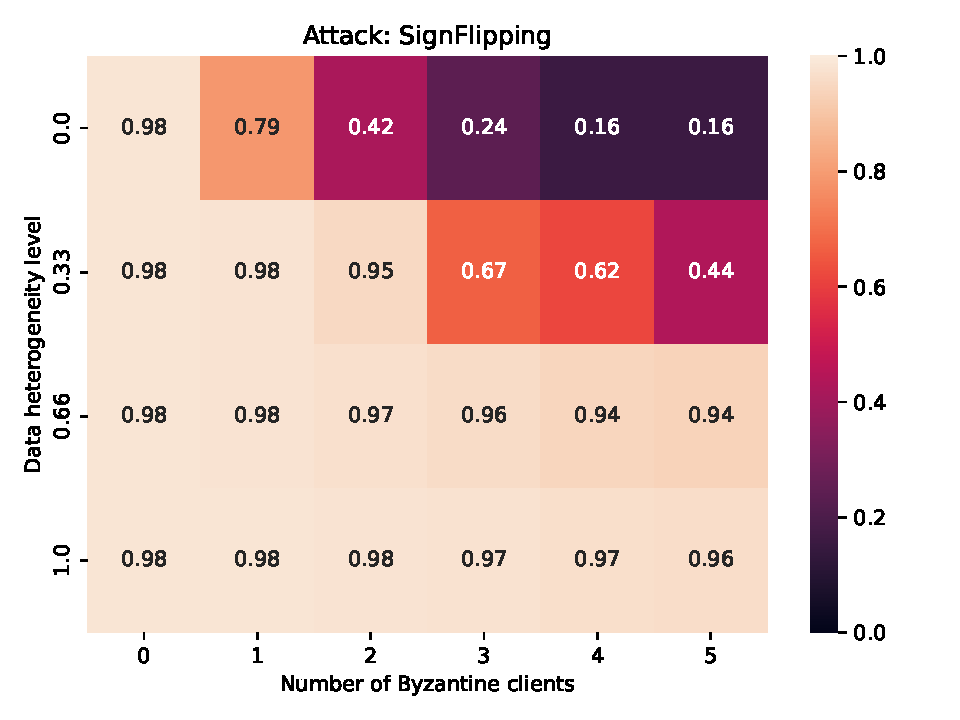
\includegraphics[width=\textwidth]{../plots/mnist_clipping_heatmaps/cnn_mnist/test_SignFlipping_mnist_cnn_mnist_gamma_similarity_niid_NNM_ARC_CenteredClipping_nb_honest_clients_10_tolerated_f_equal_real.pdf}
        \caption{No Clip (ReLU)}
        \label{fig:cc_sf_noclip}
    \end{subfigure}
    \hfill
    \begin{subfigure}[b]{0.32\textwidth}
        \centering
        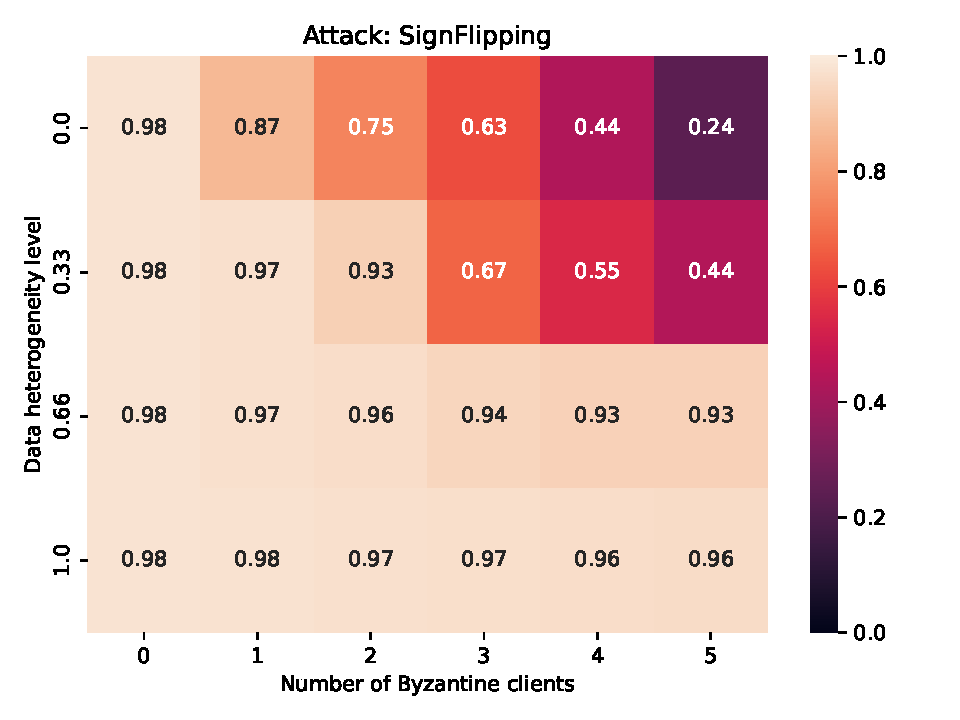
\includegraphics[width=\textwidth]{../plots/cnn_tanh_heatmaps/test_SignFlipping_mnist_cnn_mnist_tanh_gamma_similarity_niid_NNM_ARC_CenteredClipping_nb_honest_clients_10_tolerated_f_equal_real.pdf}
        \caption{Tanh}
        \label{fig:cc_sf_tanh}
    \end{subfigure}
    \hfill
    \begin{subfigure}[b]{0.32\textwidth}
        \centering
        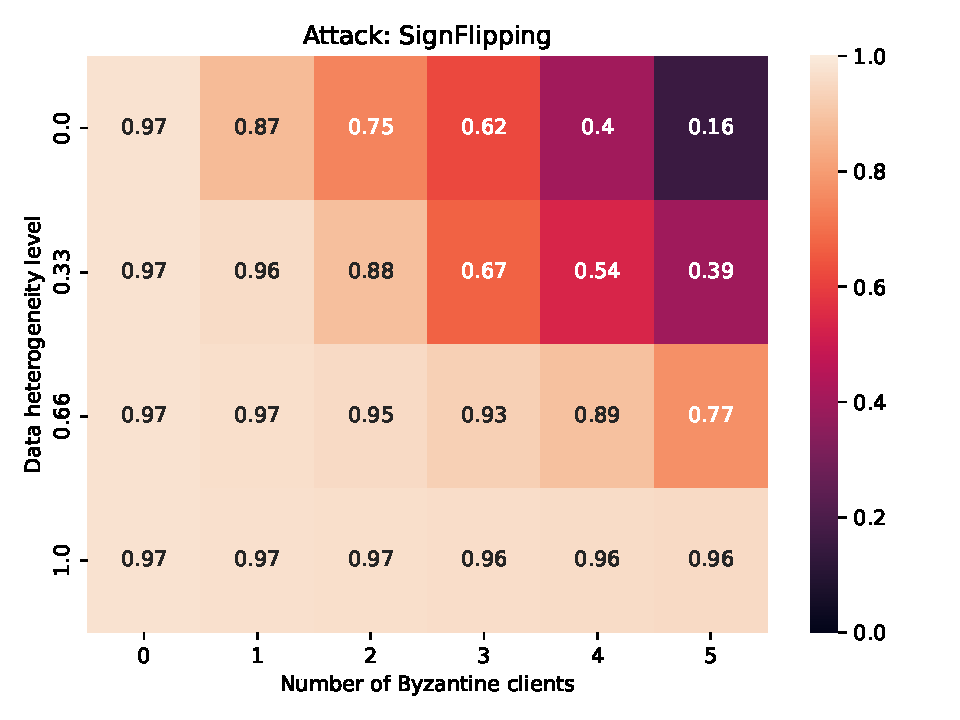
\includegraphics[width=\textwidth]{../plots/mnist_clipping_heatmaps/cnn_mnist_clipping_1/test_SignFlipping_mnist_cnn_mnist_clipping_1_gamma_similarity_niid_NNM_ARC_CenteredClipping_nb_honest_clients_10_tolerated_f_equal_real.pdf}
        \caption{Hardtanh $C{=}1$}
        \label{fig:cc_sf_hardtanh_1}
    \end{subfigure}
    \vspace{0.3cm}
    \begin{subfigure}[b]{0.32\textwidth}
        \centering
        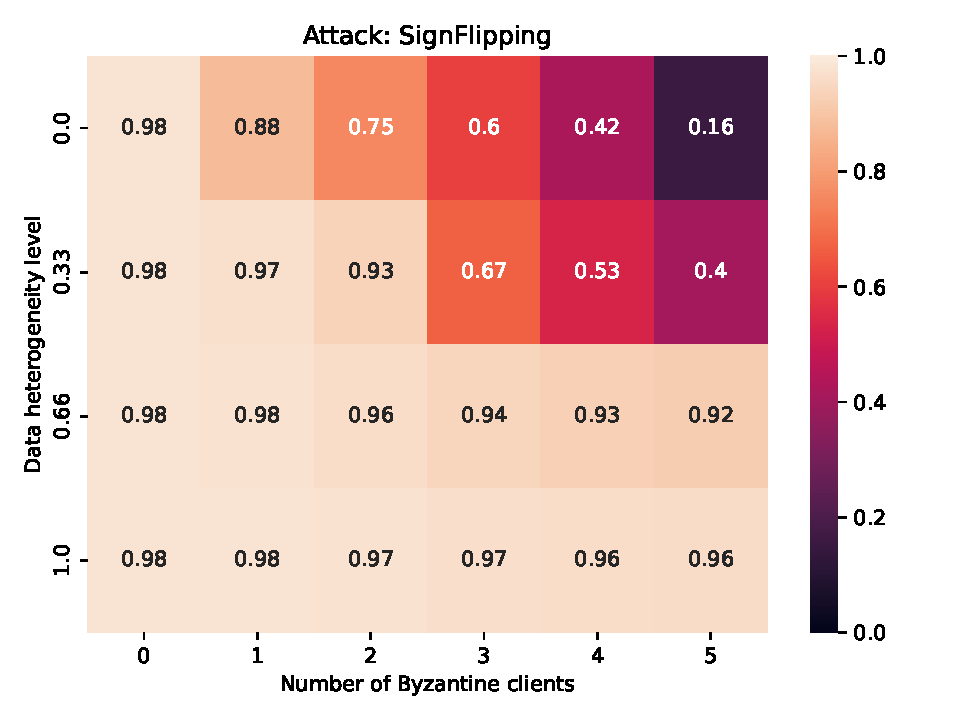
\includegraphics[width=\textwidth]{../plots/mnist_clipping_heatmaps/cnn_mnist_clipping_2/test_SignFlipping_mnist_cnn_mnist_clipping_2_gamma_similarity_niid_NNM_ARC_CenteredClipping_nb_honest_clients_10_tolerated_f_equal_real.pdf}
        \caption{Hardtanh $C{=}2$}
        \label{fig:cc_sf_hardtanh_2}
    \end{subfigure}
    \hfill
    \begin{subfigure}[b]{0.32\textwidth}
        \centering
        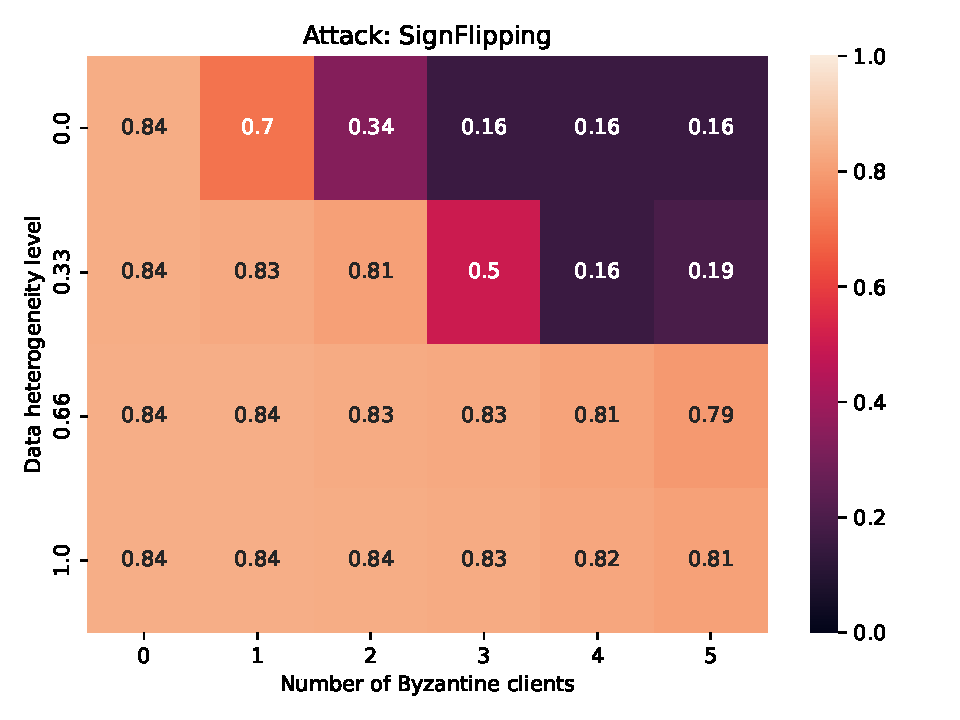
\includegraphics[width=\textwidth]{../activation_clip_plots/cnn_mnist_clip_ste_1/test_SignFlipping_mnist_cnn_mnist_clip_ste_1_gamma_similarity_niid_NNM_ARC_CenteredClipping_nb_honest_clients_10_tolerated_f_equal_real.pdf}
        \caption{STE $C{=}1$}
        \label{fig:cc_sf_ste_1}
    \end{subfigure}
    \hfill
    \begin{subfigure}[b]{0.32\textwidth}
        \centering
        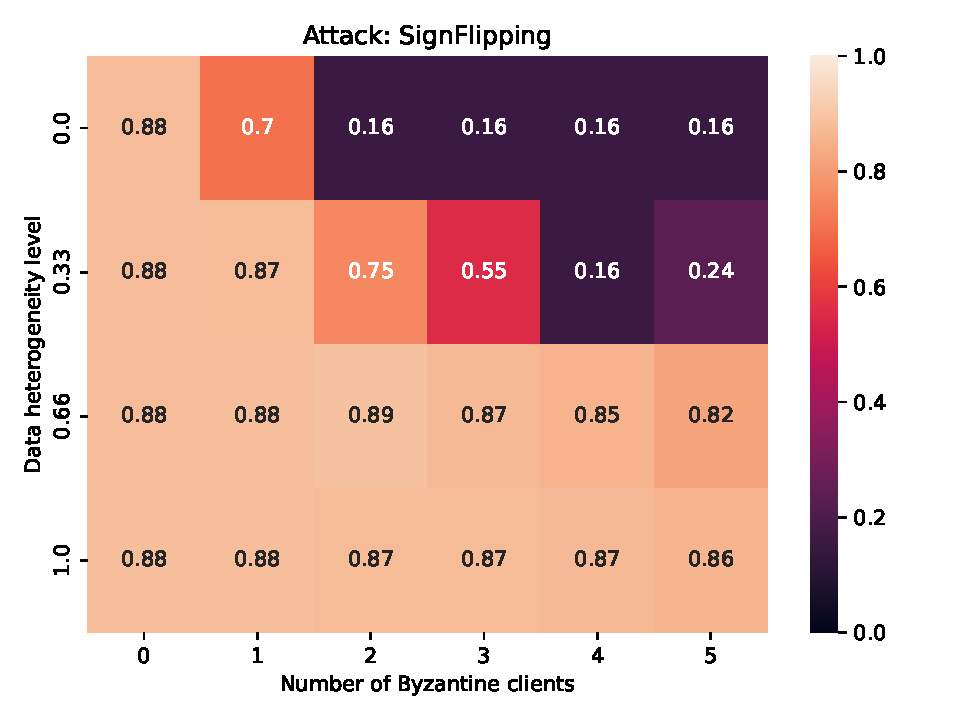
\includegraphics[width=\textwidth]{../activation_clip_plots/cnn_mnist_clip_ste_2/test_SignFlipping_mnist_cnn_mnist_clip_ste_2_gamma_similarity_niid_NNM_ARC_CenteredClipping_nb_honest_clients_10_tolerated_f_equal_real.pdf}
        \caption{STE $C{=}2$}
        \label{fig:cc_sf_ste_2}
    \end{subfigure}
    \vspace{0.3cm}
    \begin{subfigure}[b]{0.32\textwidth}
        \centering
        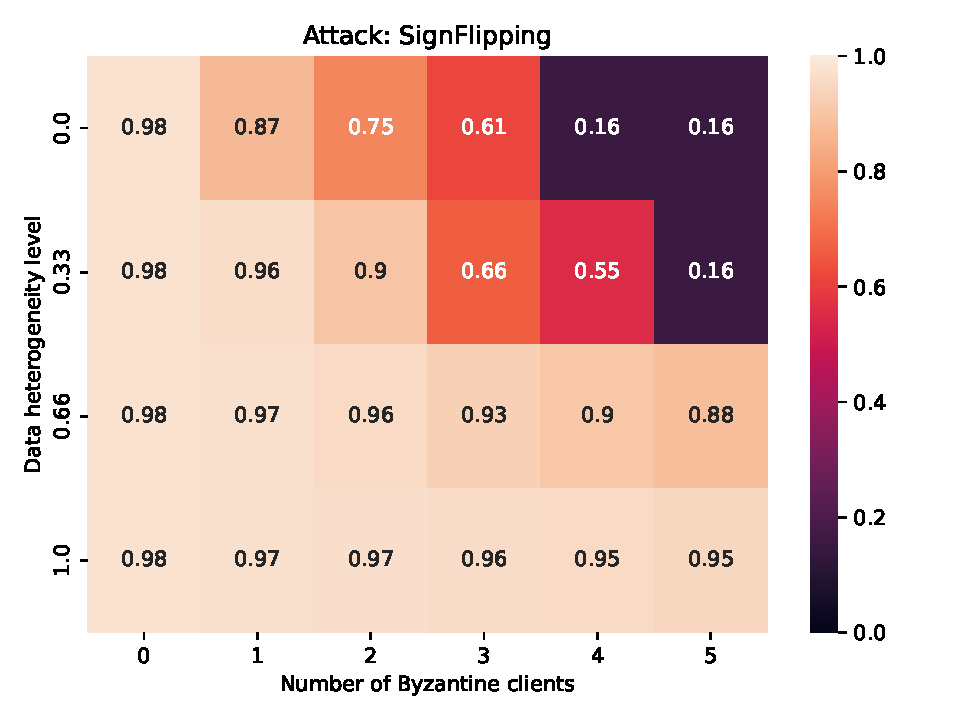
\includegraphics[width=\textwidth]{../activation_clip_plots/cnn_mnist_clip_ramp_1/test_SignFlipping_mnist_cnn_mnist_clip_ramp_1_gamma_similarity_niid_NNM_ARC_CenteredClipping_nb_honest_clients_10_tolerated_f_equal_real.pdf}
        \caption{Ramp $C{=}1$ ($r{=}2$)}
        \label{fig:cc_sf_ramp_1}
    \end{subfigure}
    \caption{Centered Clipping (CC) under Sign Flipping Attack.}
    \label{fig:cc_sf_grid}
\end{figure}
\clearpage
\subsection{CC under IPM}
\begin{figure}[htbp]
    \centering
    \begin{subfigure}[b]{0.32\textwidth}
        \centering
        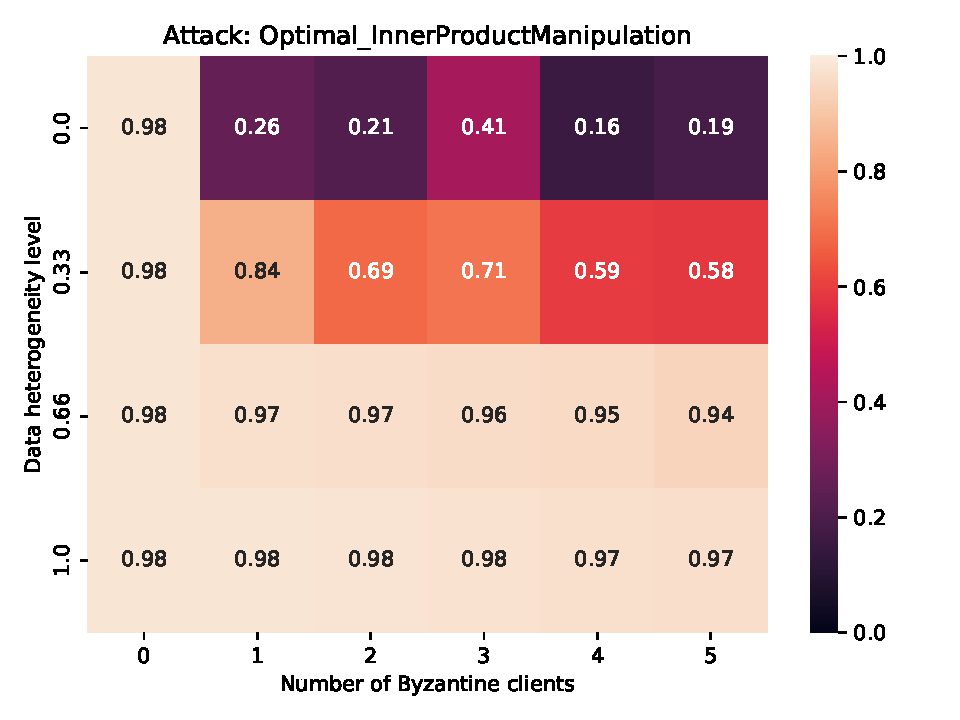
\includegraphics[width=\textwidth]{../plots/mnist_clipping_heatmaps/cnn_mnist/test_Optimal_InnerProductManipulation_mnist_cnn_mnist_gamma_similarity_niid_NNM_ARC_CenteredClipping_nb_honest_clients_10_tolerated_f_equal_real.pdf}
        \caption{No Clip (ReLU)}
        \label{fig:cc_ipm_noclip}
    \end{subfigure}
    \hfill
    \begin{subfigure}[b]{0.32\textwidth}
        \centering
        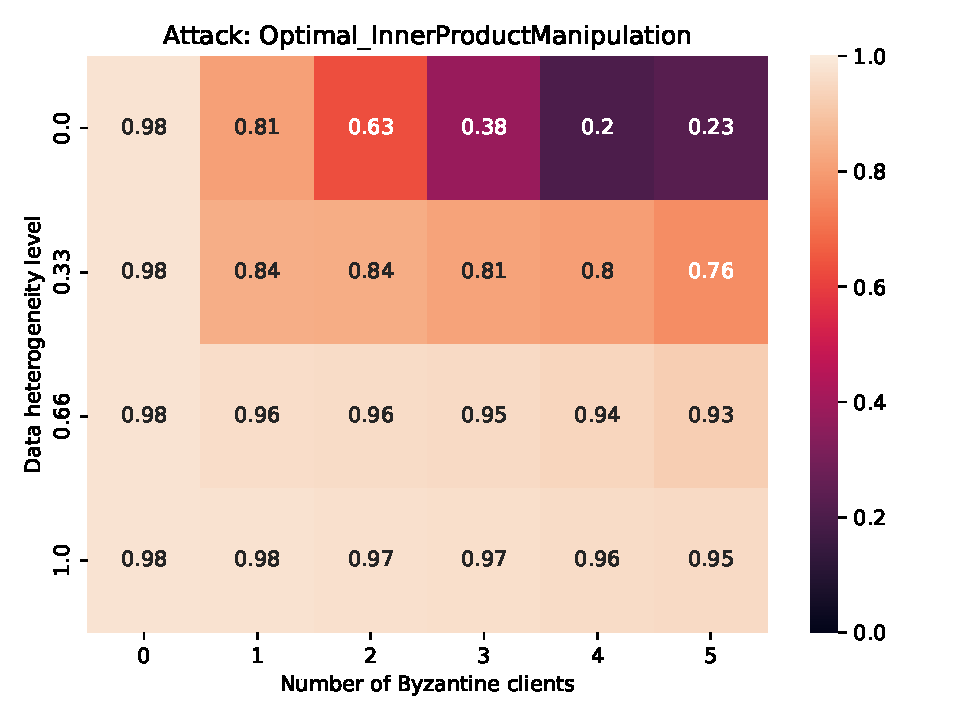
\includegraphics[width=\textwidth]{../plots/cnn_tanh_heatmaps/test_Optimal_InnerProductManipulation_mnist_cnn_mnist_tanh_gamma_similarity_niid_NNM_ARC_CenteredClipping_nb_honest_clients_10_tolerated_f_equal_real.pdf}
        \caption{Tanh}
        \label{fig:cc_ipm_tanh}
    \end{subfigure}
    \hfill
    \begin{subfigure}[b]{0.32\textwidth}
        \centering
        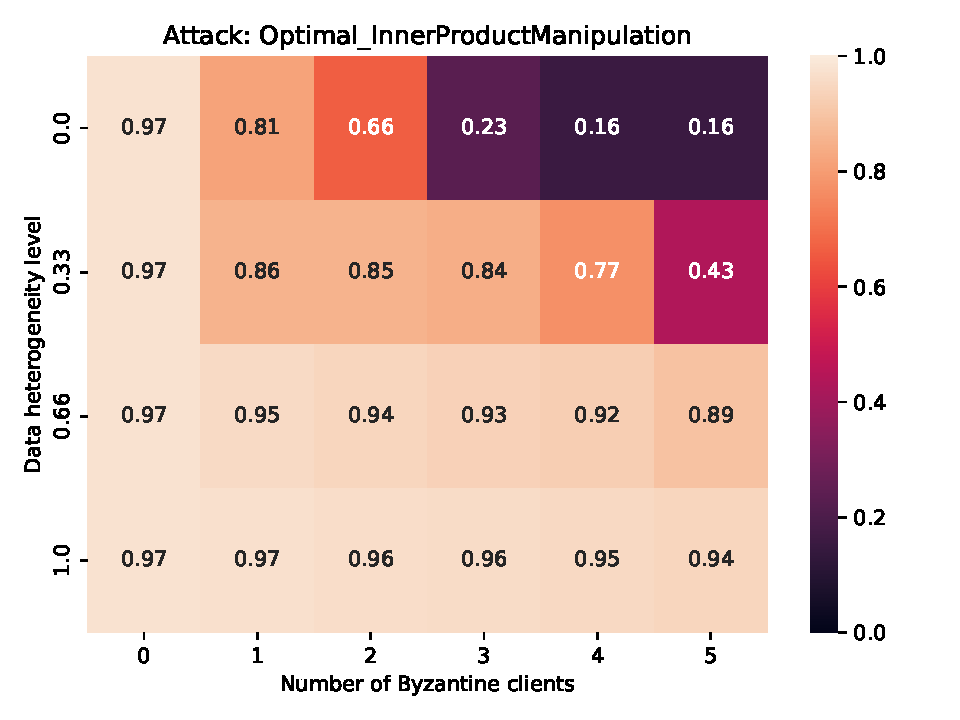
\includegraphics[width=\textwidth]{../plots/mnist_clipping_heatmaps/cnn_mnist_clipping_1/test_Optimal_InnerProductManipulation_mnist_cnn_mnist_clipping_1_gamma_similarity_niid_NNM_ARC_CenteredClipping_nb_honest_clients_10_tolerated_f_equal_real.pdf}
        \caption{Hardtanh $C{=}1$}
        \label{fig:cc_ipm_hardtanh_1}
    \end{subfigure}
    \vspace{0.3cm}
    \begin{subfigure}[b]{0.32\textwidth}
        \centering
        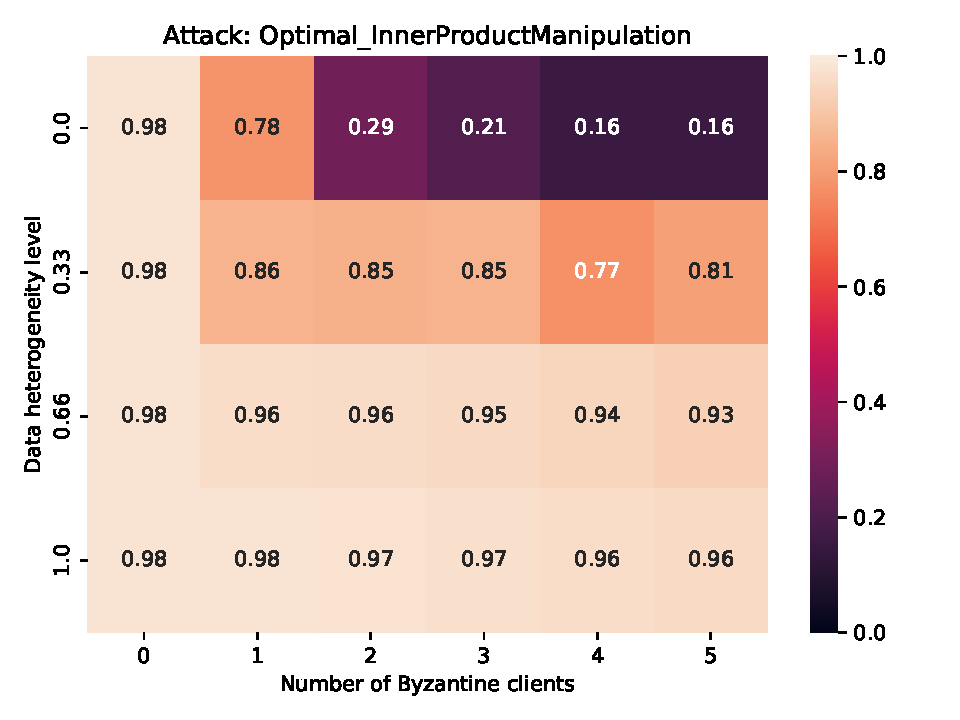
\includegraphics[width=\textwidth]{../plots/mnist_clipping_heatmaps/cnn_mnist_clipping_2/test_Optimal_InnerProductManipulation_mnist_cnn_mnist_clipping_2_gamma_similarity_niid_NNM_ARC_CenteredClipping_nb_honest_clients_10_tolerated_f_equal_real.pdf}
        \caption{Hardtanh $C{=}2$}
        \label{fig:cc_ipm_hardtanh_2}
    \end{subfigure}
    \hfill
    \begin{subfigure}[b]{0.32\textwidth}
        \centering
        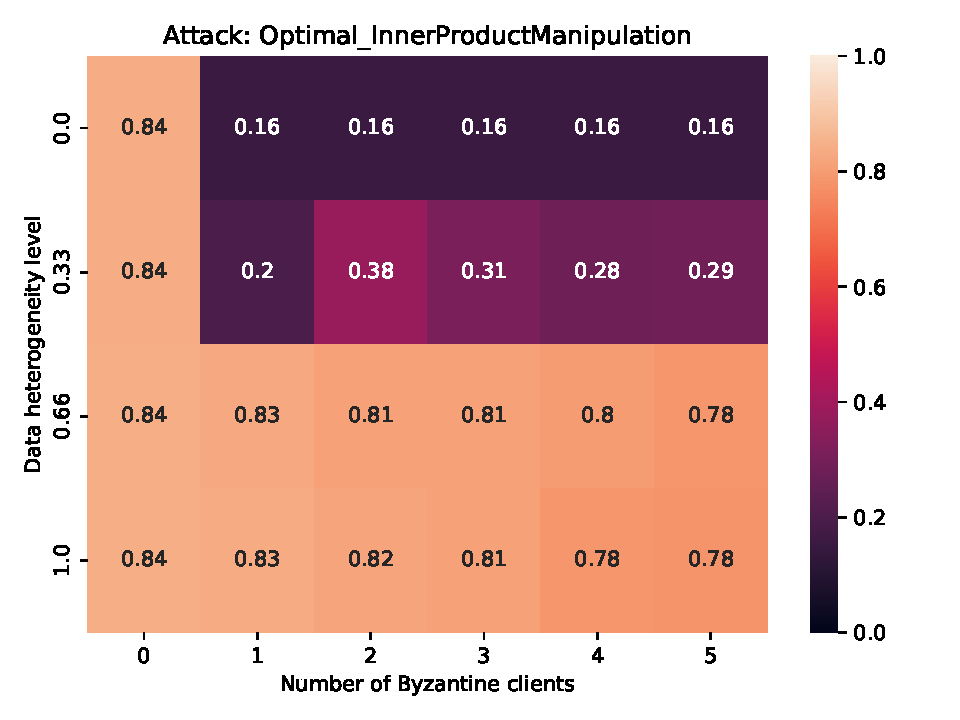
\includegraphics[width=\textwidth]{../activation_clip_plots/cnn_mnist_clip_ste_1/test_Optimal_InnerProductManipulation_mnist_cnn_mnist_clip_ste_1_gamma_similarity_niid_NNM_ARC_CenteredClipping_nb_honest_clients_10_tolerated_f_equal_real.pdf}
        \caption{STE $C{=}1$}
        \label{fig:cc_ipm_ste_1}
    \end{subfigure}
    \hfill
    \begin{subfigure}[b]{0.32\textwidth}
        \centering
        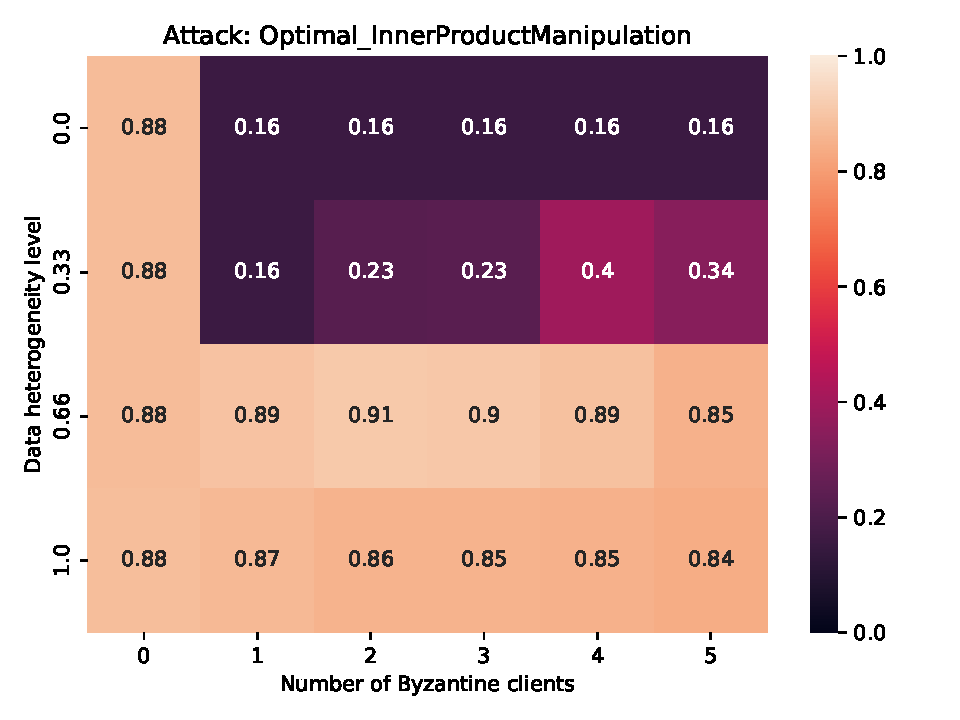
\includegraphics[width=\textwidth]{../activation_clip_plots/cnn_mnist_clip_ste_2/test_Optimal_InnerProductManipulation_mnist_cnn_mnist_clip_ste_2_gamma_similarity_niid_NNM_ARC_CenteredClipping_nb_honest_clients_10_tolerated_f_equal_real.pdf}
        \caption{STE $C{=}2$}
        \label{fig:cc_ipm_ste_2}
    \end{subfigure}
    \vspace{0.3cm}
    \begin{subfigure}[b]{0.32\textwidth}
        \centering
        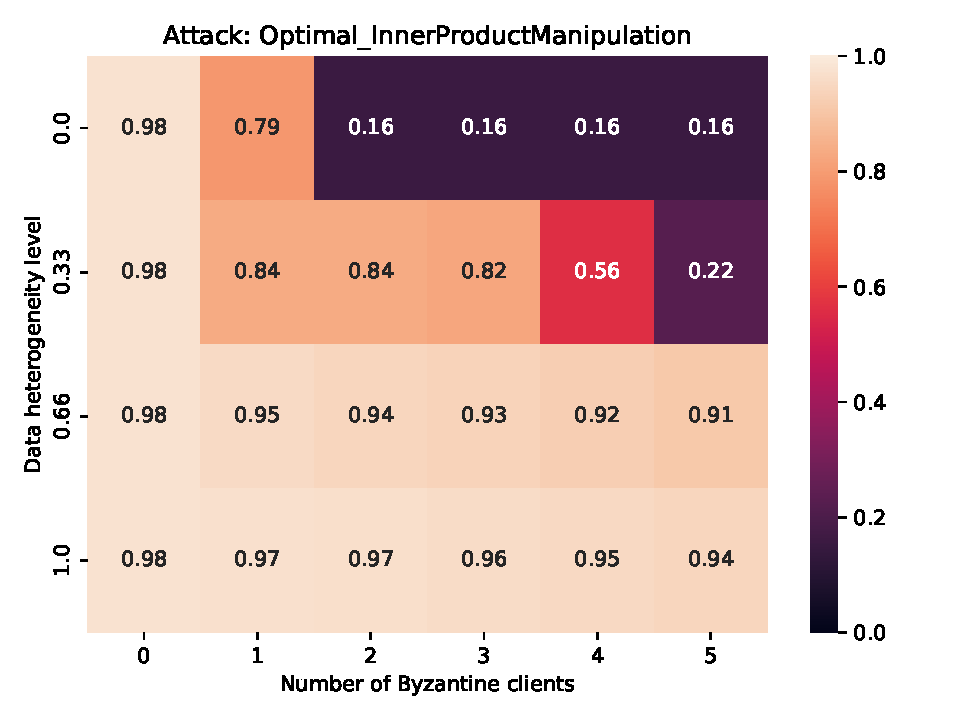
\includegraphics[width=\textwidth]{../activation_clip_plots/cnn_mnist_clip_ramp_1/test_Optimal_InnerProductManipulation_mnist_cnn_mnist_clip_ramp_1_gamma_similarity_niid_NNM_ARC_CenteredClipping_nb_honest_clients_10_tolerated_f_equal_real.pdf}
        \caption{Ramp $C{=}1$ ($r{=}2$)}
        \label{fig:cc_ipm_ramp_1}
    \end{subfigure}
    \caption{Centered Clipping (CC) under Optimal IPM Attack.}
    \label{fig:cc_ipm_grid}
\end{figure}
\clearpage
\section{Geometric Median (GM)}
\subsection{GM under Worst-Case across all Attacks}
\begin{figure}[htbp]
    \centering
    \begin{subfigure}[b]{0.32\textwidth}
        \centering
        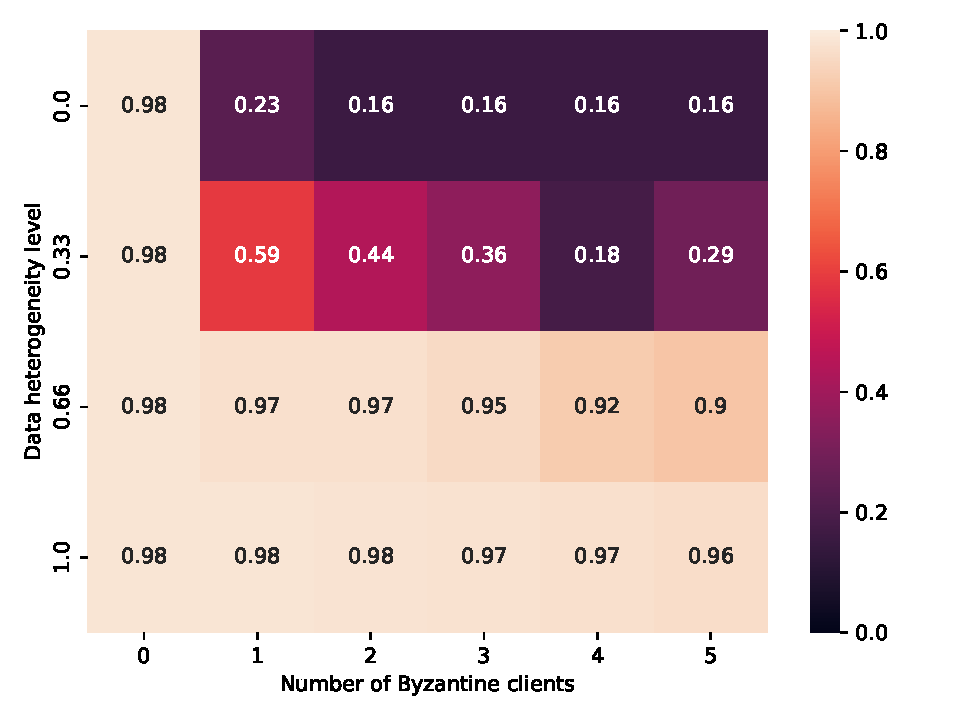
\includegraphics[width=\textwidth]{../plots/mnist_clipping_heatmaps/cnn_mnist/test_mnist_cnn_mnist_gamma_similarity_niid_NNM_ARC_GeometricMedian_nb_honest_clients_10_tolerated_f_equal_real.pdf}
        \caption{No Clip (ReLU)}
        \label{fig:gm_worst_case_noclip}
    \end{subfigure}
    \hfill
    \begin{subfigure}[b]{0.32\textwidth}
        \centering
        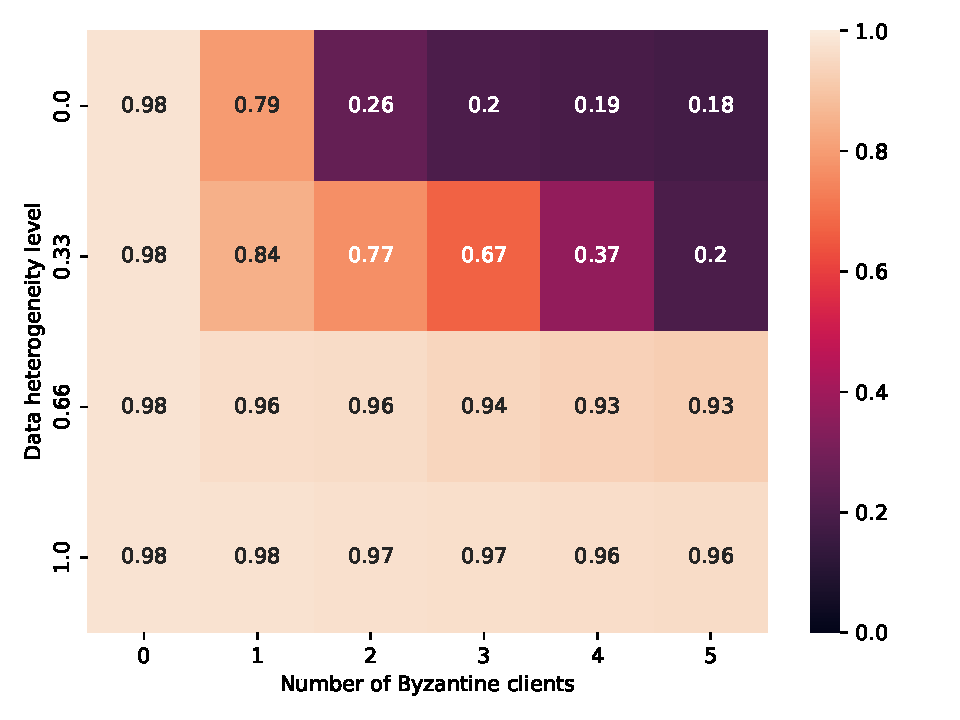
\includegraphics[width=\textwidth]{../plots/cnn_tanh_heatmaps/test_mnist_cnn_mnist_tanh_gamma_similarity_niid_NNM_ARC_GeometricMedian_nb_honest_clients_10_tolerated_f_equal_real.pdf}
        \caption{Tanh}
        \label{fig:gm_worst_case_tanh}
    \end{subfigure}
    \hfill
    \begin{subfigure}[b]{0.32\textwidth}
        \centering
        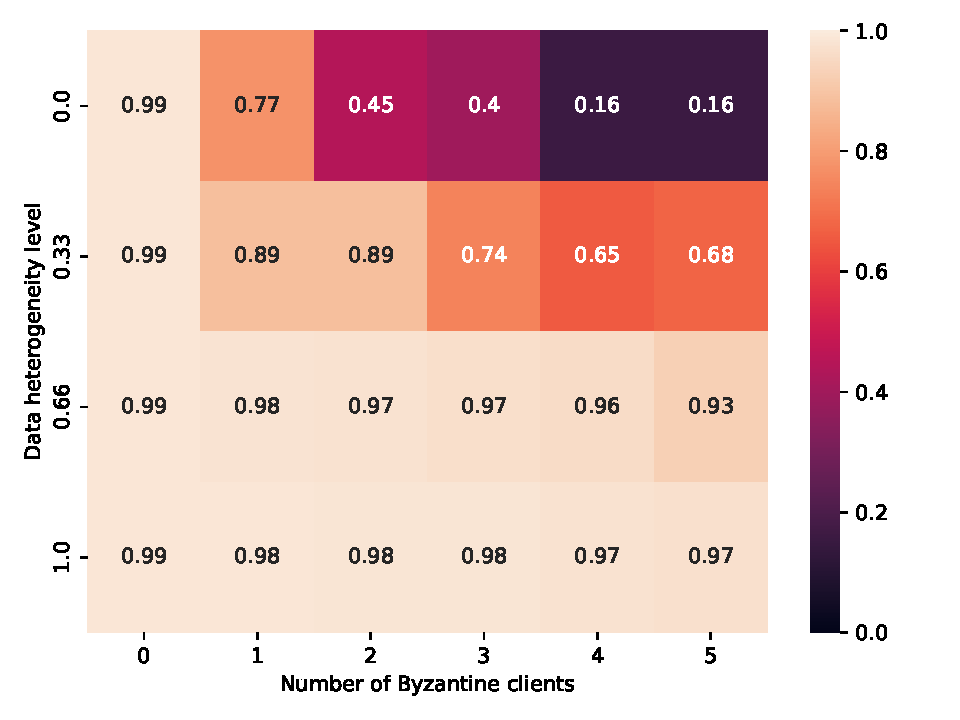
\includegraphics[width=\textwidth]{../plots/cnn_clipped_heatmaps/test_mnist_cnn_mnist_gamma_similarity_niid_NNM_ARC_GeometricMedian_nb_honest_clients_10_tolerated_f_equal_real.pdf}
        \caption{Grad-Norm Clip $=21$}
        \label{fig:gm_worst_case_gradnorm21}
    \end{subfigure}
    \vspace{0.3cm}
    \begin{subfigure}[b]{0.32\textwidth}
        \centering
        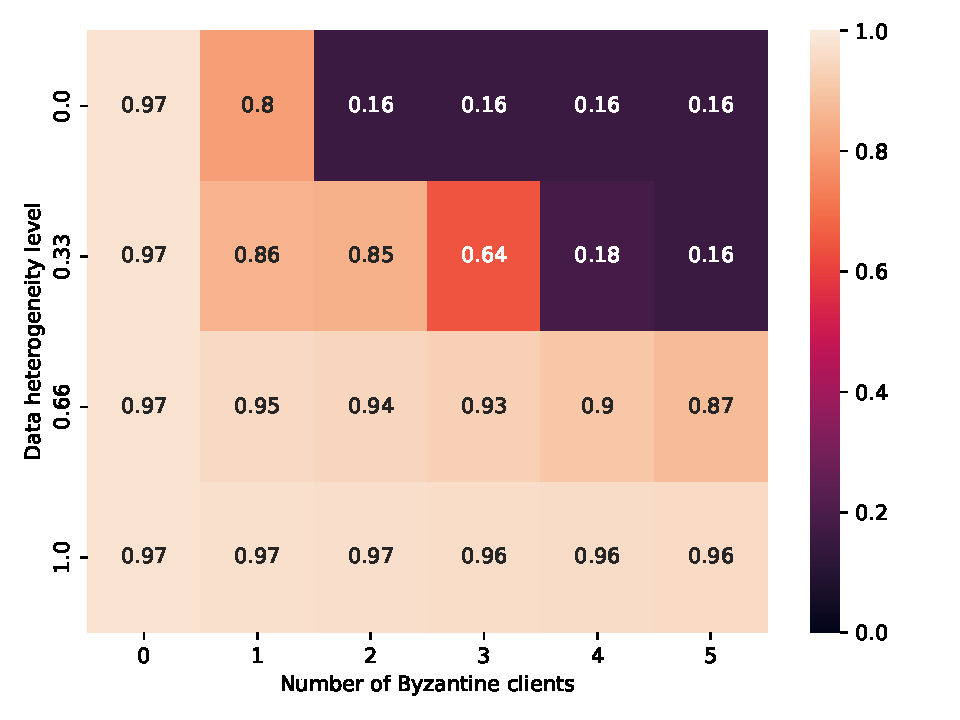
\includegraphics[width=\textwidth]{../plots/mnist_clipping_heatmaps/cnn_mnist_clipping_1/test_mnist_cnn_mnist_clipping_1_gamma_similarity_niid_NNM_ARC_GeometricMedian_nb_honest_clients_10_tolerated_f_equal_real.pdf}
        \caption{Hardtanh $C{=}1$}
        \label{fig:gm_worst_case_hardtanh_1}
    \end{subfigure}
    \hfill
    \begin{subfigure}[b]{0.32\textwidth}
        \centering
        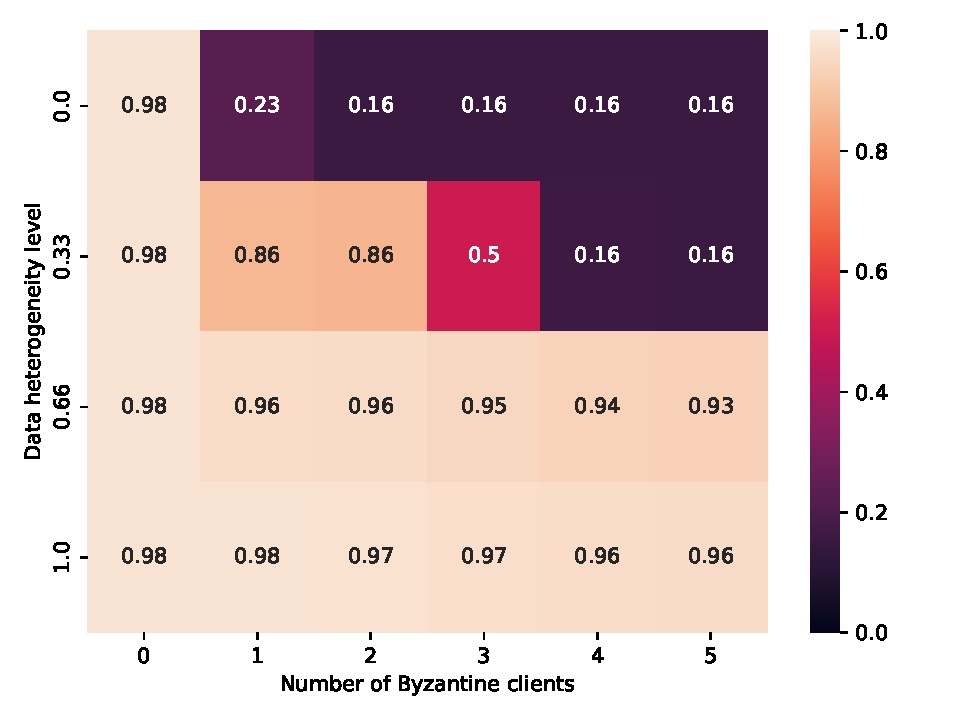
\includegraphics[width=\textwidth]{../plots/mnist_clipping_heatmaps/cnn_mnist_clipping_2/test_mnist_cnn_mnist_clipping_2_gamma_similarity_niid_NNM_ARC_GeometricMedian_nb_honest_clients_10_tolerated_f_equal_real.pdf}
        \caption{Hardtanh $C{=}2$}
        \label{fig:gm_worst_case_hardtanh_2}
    \end{subfigure}
    \hfill
    \begin{subfigure}[b]{0.32\textwidth}
        \centering
        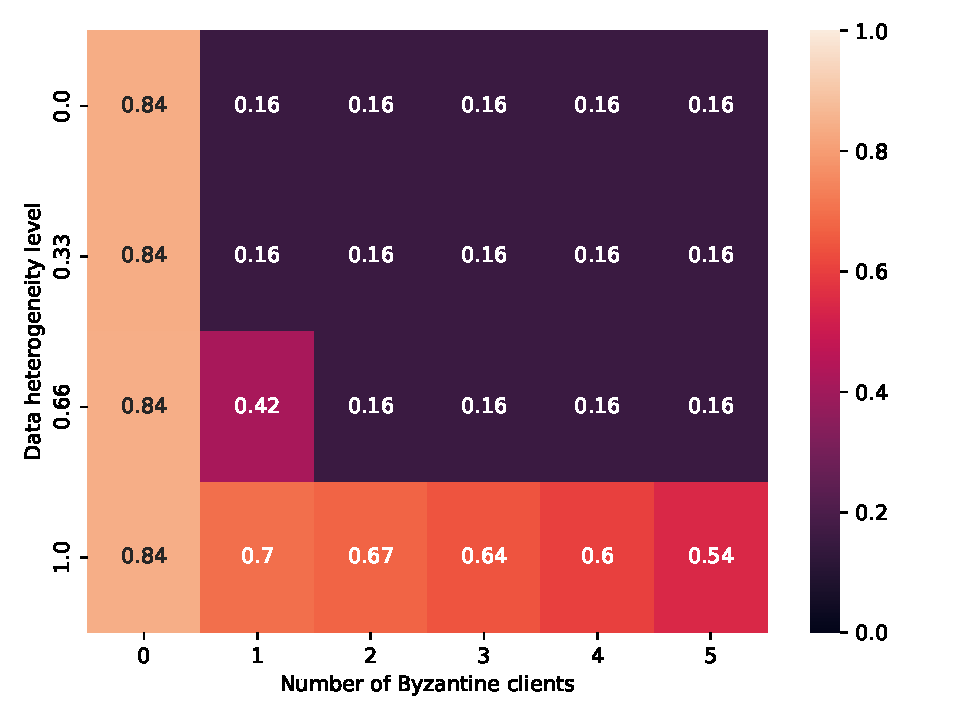
\includegraphics[width=\textwidth]{../activation_clip_plots/cnn_mnist_clip_ste_1/test_mnist_cnn_mnist_clip_ste_1_gamma_similarity_niid_NNM_ARC_GeometricMedian_nb_honest_clients_10_tolerated_f_equal_real.pdf}
        \caption{STE $C{=}1$}
        \label{fig:gm_worst_case_ste_1}
    \end{subfigure}
    \vspace{0.3cm}
    \begin{subfigure}[b]{0.32\textwidth}
        \centering
        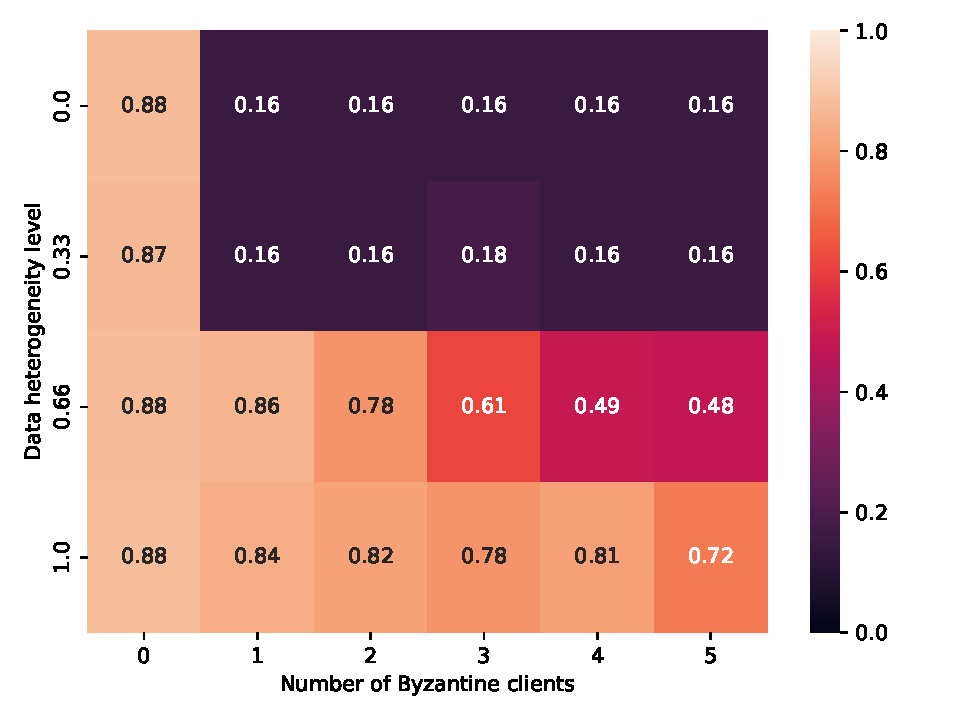
\includegraphics[width=\textwidth]{../activation_clip_plots/cnn_mnist_clip_ste_2/test_mnist_cnn_mnist_clip_ste_2_gamma_similarity_niid_NNM_ARC_GeometricMedian_nb_honest_clients_10_tolerated_f_equal_real.pdf}
        \caption{STE $C{=}2$}
        \label{fig:gm_worst_case_ste_2}
    \end{subfigure}
    \hfill
    \begin{subfigure}[b]{0.32\textwidth}
        \centering
        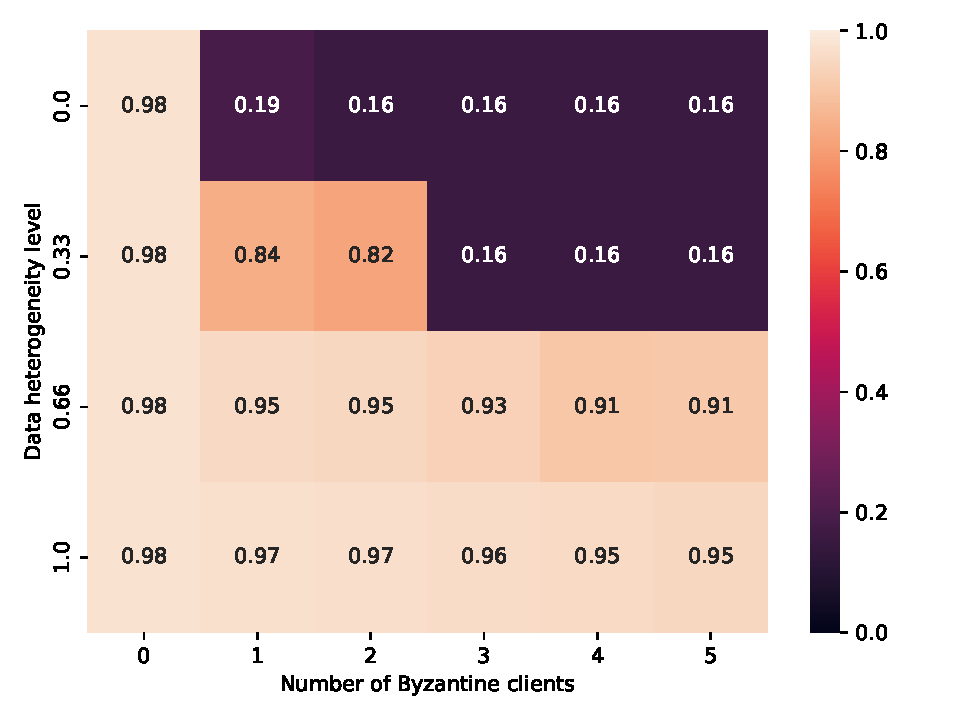
\includegraphics[width=\textwidth]{../activation_clip_plots/cnn_mnist_clip_ramp_1/test_mnist_cnn_mnist_clip_ramp_1_gamma_similarity_niid_NNM_ARC_GeometricMedian_nb_honest_clients_10_tolerated_f_equal_real.pdf}
        \caption{Ramp $C{=}1$ ($r{=}2$)}
        \label{fig:gm_worst_case_ramp_1}
    \end{subfigure}
    \caption{Geometric Median (GM) under Worst-Case across all Attacks.}
    \label{fig:gm_worst_case_grid}
\end{figure}
\clearpage
\subsection{GM under ALIE}
\begin{figure}[htbp]
    \centering
    \begin{subfigure}[b]{0.32\textwidth}
        \centering
        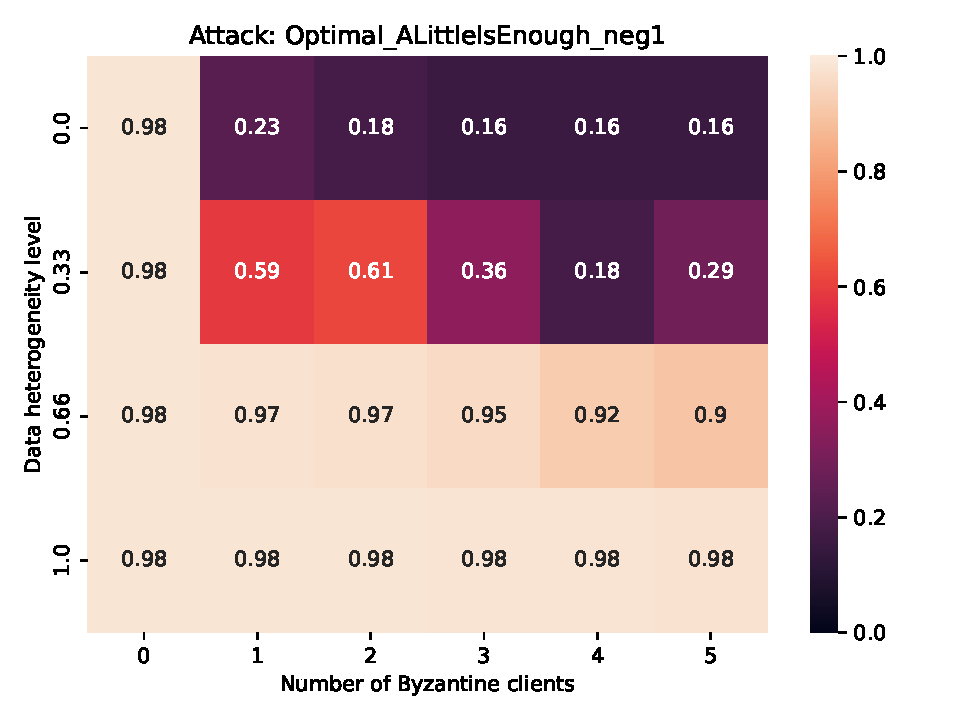
\includegraphics[width=\textwidth]{../plots/mnist_clipping_heatmaps/cnn_mnist/test_Optimal_ALittleIsEnough_neg1_mnist_cnn_mnist_gamma_similarity_niid_NNM_ARC_GeometricMedian_nb_honest_clients_10_tolerated_f_equal_real.pdf}
        \caption{No Clip (ReLU)}
        \label{fig:gm_alie_noclip}
    \end{subfigure}
    \hfill
    \begin{subfigure}[b]{0.32\textwidth}
        \centering
        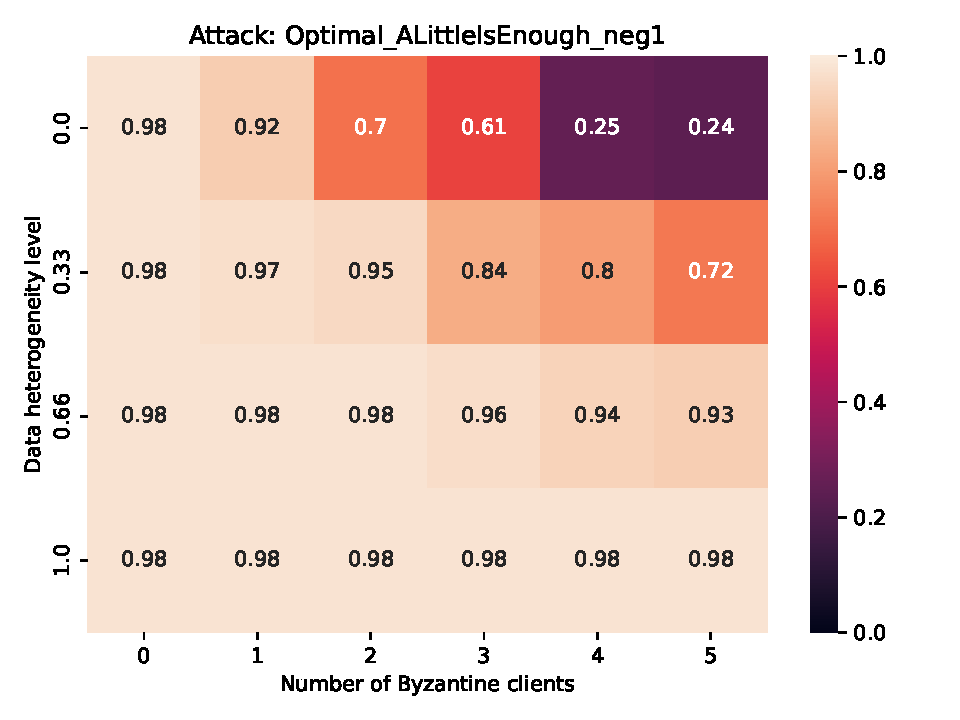
\includegraphics[width=\textwidth]{../plots/cnn_tanh_heatmaps/test_Optimal_ALittleIsEnough_neg1_mnist_cnn_mnist_tanh_gamma_similarity_niid_NNM_ARC_GeometricMedian_nb_honest_clients_10_tolerated_f_equal_real.pdf}
        \caption{Tanh}
        \label{fig:gm_alie_tanh}
    \end{subfigure}
    \hfill
    \begin{subfigure}[b]{0.32\textwidth}
        \centering
        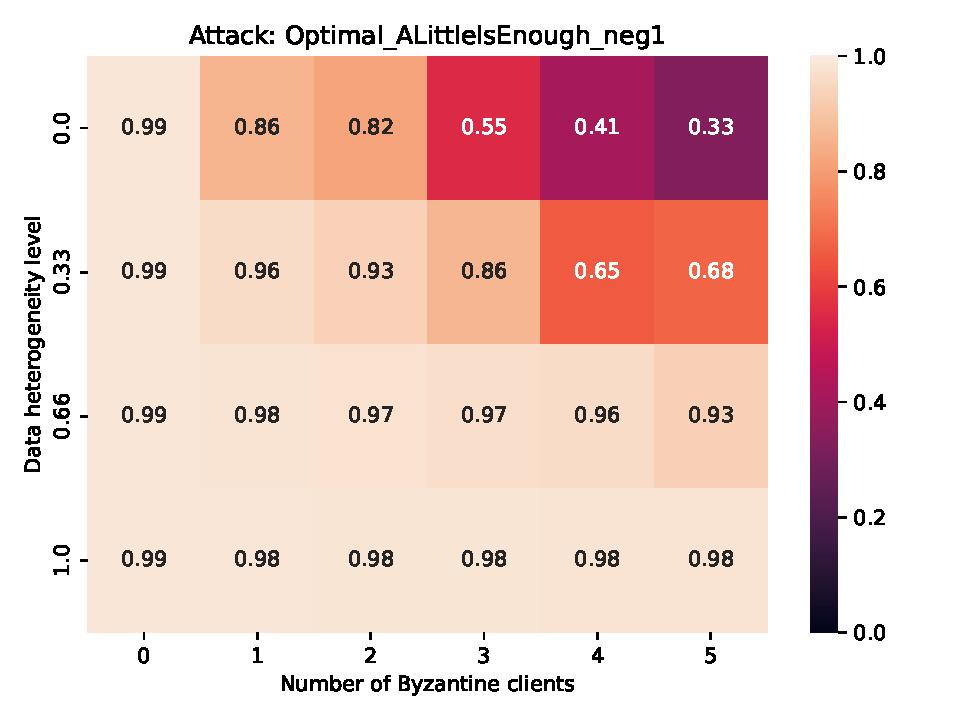
\includegraphics[width=\textwidth]{../plots/cnn_clipped_heatmaps/test_Optimal_ALittleIsEnough_neg1_mnist_cnn_mnist_gamma_similarity_niid_NNM_ARC_GeometricMedian_nb_honest_clients_10_tolerated_f_equal_real.pdf}
        \caption{Grad-Norm Clip $=21$}
        \label{fig:gm_alie_gradnorm21}
    \end{subfigure}
    \vspace{0.3cm}
    \begin{subfigure}[b]{0.32\textwidth}
        \centering
        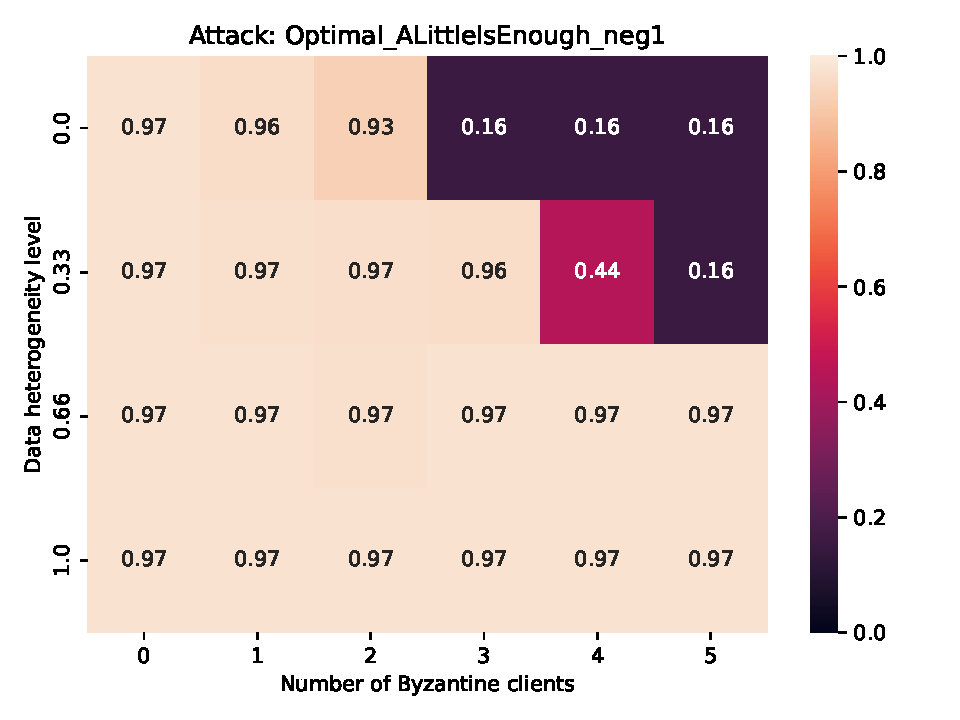
\includegraphics[width=\textwidth]{../plots/mnist_clipping_heatmaps/cnn_mnist_clipping_1/test_Optimal_ALittleIsEnough_neg1_mnist_cnn_mnist_clipping_1_gamma_similarity_niid_NNM_ARC_GeometricMedian_nb_honest_clients_10_tolerated_f_equal_real.pdf}
        \caption{Hardtanh $C{=}1$}
        \label{fig:gm_alie_hardtanh_1}
    \end{subfigure}
    \hfill
    \begin{subfigure}[b]{0.32\textwidth}
        \centering
        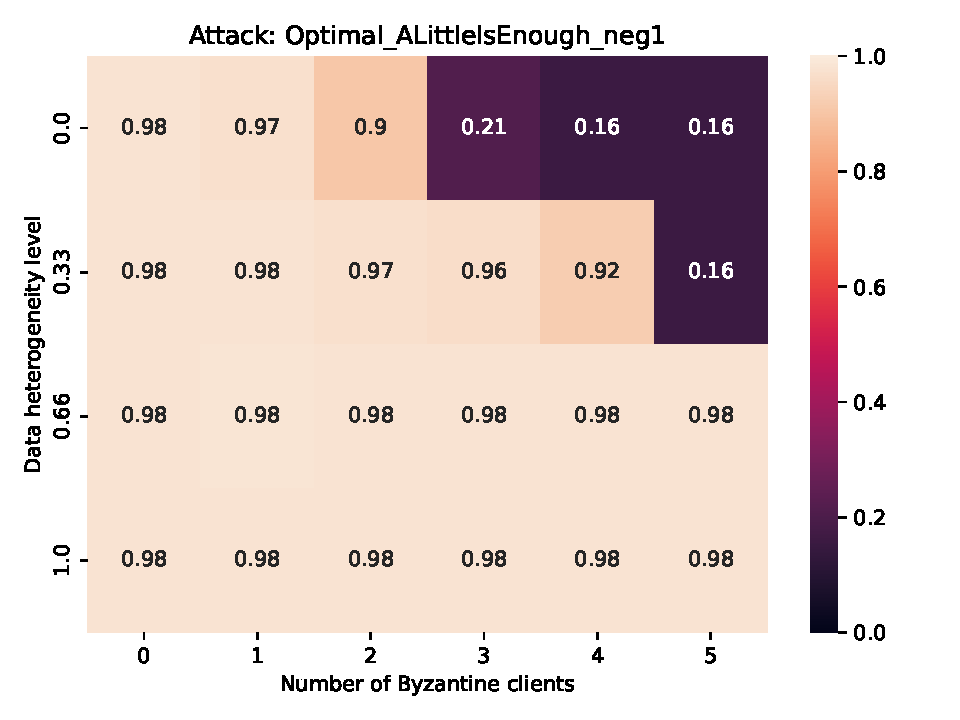
\includegraphics[width=\textwidth]{../plots/mnist_clipping_heatmaps/cnn_mnist_clipping_2/test_Optimal_ALittleIsEnough_neg1_mnist_cnn_mnist_clipping_2_gamma_similarity_niid_NNM_ARC_GeometricMedian_nb_honest_clients_10_tolerated_f_equal_real.pdf}
        \caption{Hardtanh $C{=}2$}
        \label{fig:gm_alie_hardtanh_2}
    \end{subfigure}
    \hfill
    \begin{subfigure}[b]{0.32\textwidth}
        \centering
        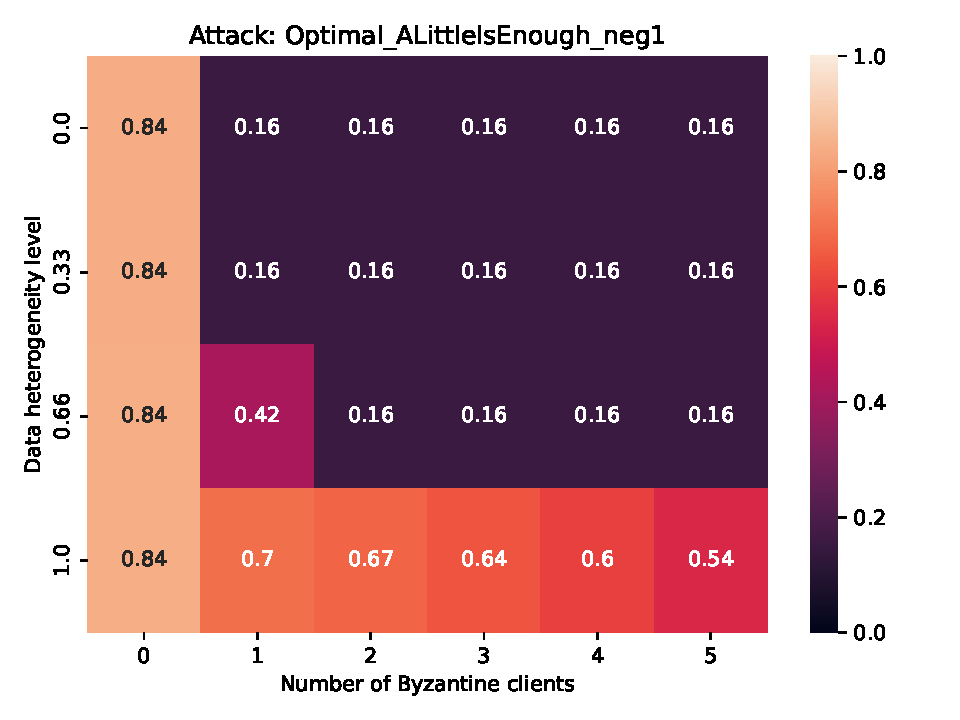
\includegraphics[width=\textwidth]{../activation_clip_plots/cnn_mnist_clip_ste_1/test_Optimal_ALittleIsEnough_neg1_mnist_cnn_mnist_clip_ste_1_gamma_similarity_niid_NNM_ARC_GeometricMedian_nb_honest_clients_10_tolerated_f_equal_real.pdf}
        \caption{STE $C{=}1$}
        \label{fig:gm_alie_ste_1}
    \end{subfigure}
    \vspace{0.3cm}
    \begin{subfigure}[b]{0.32\textwidth}
        \centering
        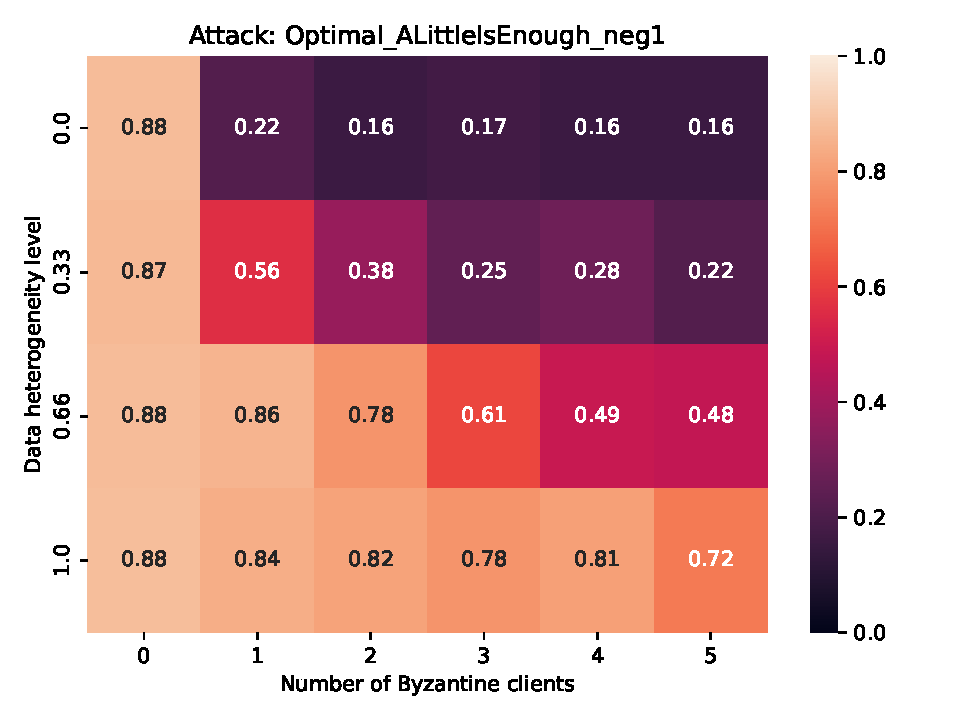
\includegraphics[width=\textwidth]{../activation_clip_plots/cnn_mnist_clip_ste_2/test_Optimal_ALittleIsEnough_neg1_mnist_cnn_mnist_clip_ste_2_gamma_similarity_niid_NNM_ARC_GeometricMedian_nb_honest_clients_10_tolerated_f_equal_real.pdf}
        \caption{STE $C{=}2$}
        \label{fig:gm_alie_ste_2}
    \end{subfigure}
    \hfill
    \begin{subfigure}[b]{0.32\textwidth}
        \centering
        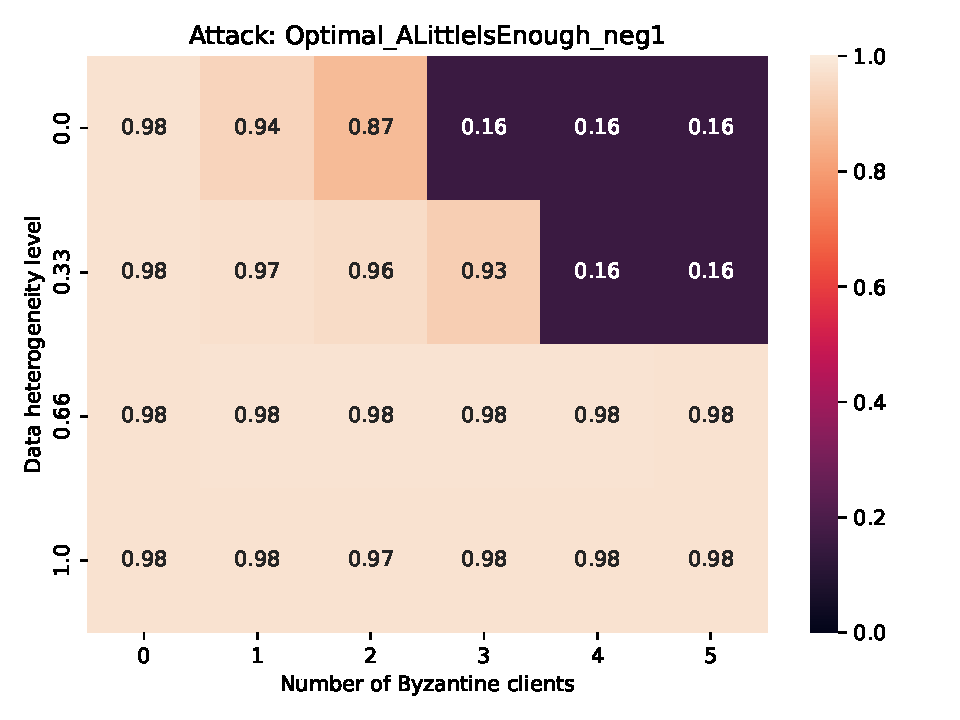
\includegraphics[width=\textwidth]{../activation_clip_plots/cnn_mnist_clip_ramp_1/test_Optimal_ALittleIsEnough_neg1_mnist_cnn_mnist_clip_ramp_1_gamma_similarity_niid_NNM_ARC_GeometricMedian_nb_honest_clients_10_tolerated_f_equal_real.pdf}
        \caption{Ramp $C{=}1$ ($r{=}2$)}
        \label{fig:gm_alie_ramp_1}
    \end{subfigure}
    \caption{Geometric Median (GM) under Optimal ALIE Attack.}
    \label{fig:gm_alie_grid}
\end{figure}
\clearpage
\subsection{GM under SF}
\begin{figure}[htbp]
    \centering
    \begin{subfigure}[b]{0.32\textwidth}
        \centering
        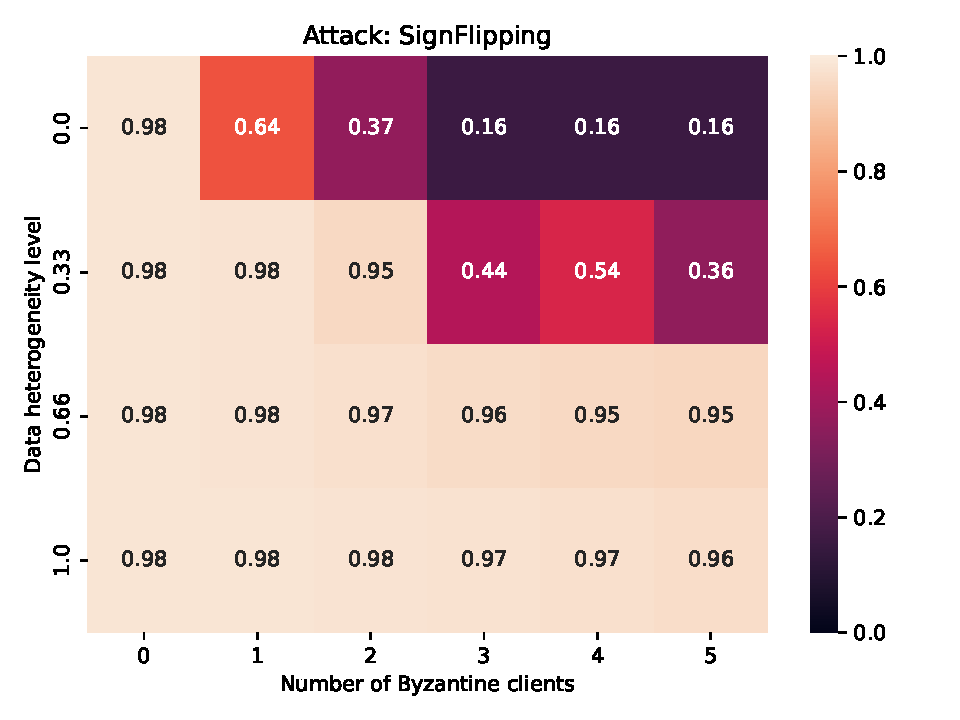
\includegraphics[width=\textwidth]{../plots/mnist_clipping_heatmaps/cnn_mnist/test_SignFlipping_mnist_cnn_mnist_gamma_similarity_niid_NNM_ARC_GeometricMedian_nb_honest_clients_10_tolerated_f_equal_real.pdf}
        \caption{No Clip (ReLU)}
        \label{fig:gm_sf_noclip}
    \end{subfigure}
    \hfill
    \begin{subfigure}[b]{0.32\textwidth}
        \centering
        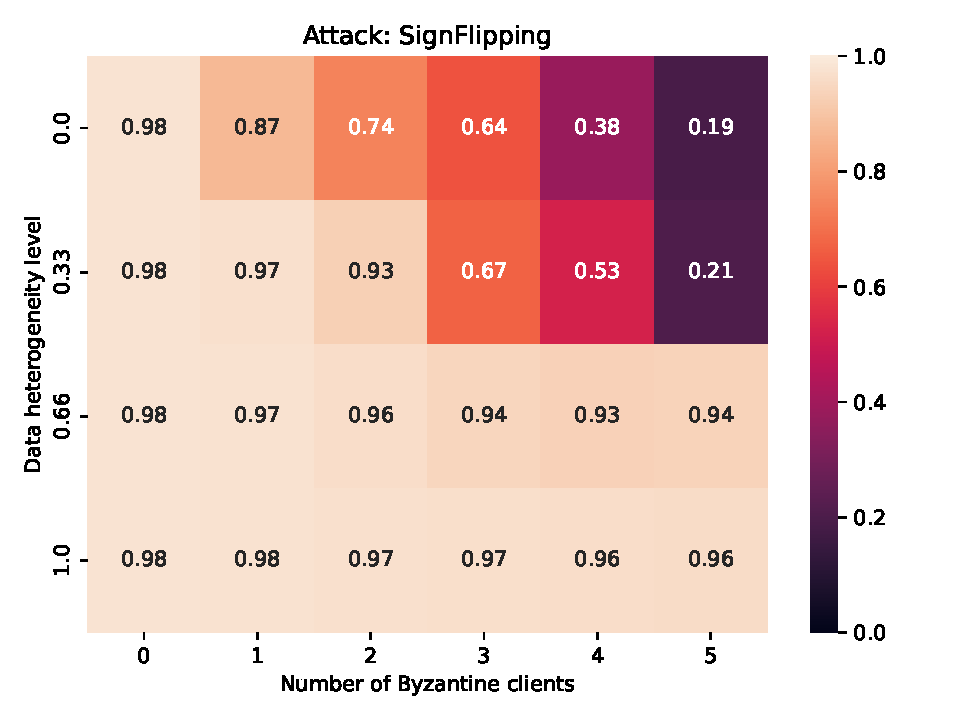
\includegraphics[width=\textwidth]{../plots/cnn_tanh_heatmaps/test_SignFlipping_mnist_cnn_mnist_tanh_gamma_similarity_niid_NNM_ARC_GeometricMedian_nb_honest_clients_10_tolerated_f_equal_real.pdf}
        \caption{Tanh}
        \label{fig:gm_sf_tanh}
    \end{subfigure}
    \hfill
    \begin{subfigure}[b]{0.32\textwidth}
        \centering
        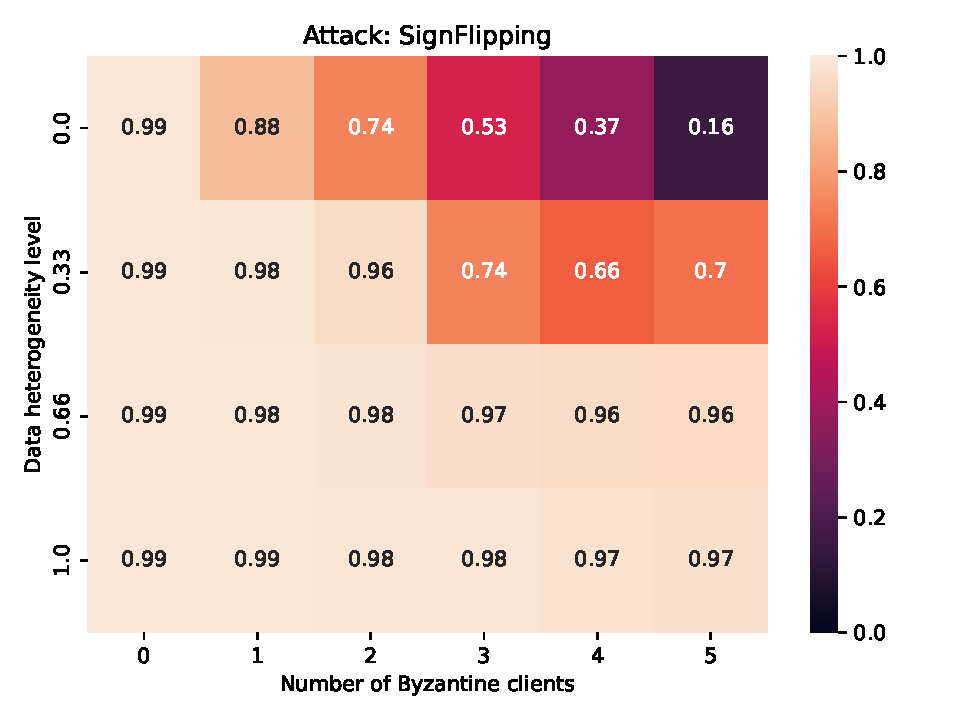
\includegraphics[width=\textwidth]{../plots/cnn_clipped_heatmaps/test_SignFlipping_mnist_cnn_mnist_gamma_similarity_niid_NNM_ARC_GeometricMedian_nb_honest_clients_10_tolerated_f_equal_real.pdf}
        \caption{Grad-Norm Clip $=21$}
        \label{fig:gm_sf_gradnorm21}
    \end{subfigure}
    \vspace{0.3cm}
    \begin{subfigure}[b]{0.32\textwidth}
        \centering
        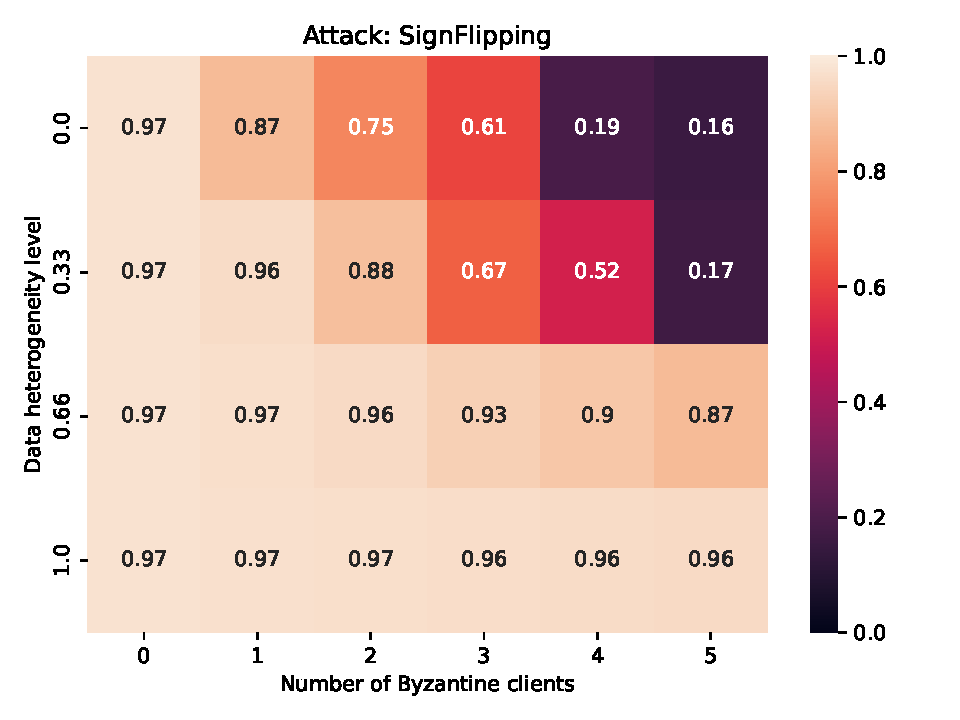
\includegraphics[width=\textwidth]{../plots/mnist_clipping_heatmaps/cnn_mnist_clipping_1/test_SignFlipping_mnist_cnn_mnist_clipping_1_gamma_similarity_niid_NNM_ARC_GeometricMedian_nb_honest_clients_10_tolerated_f_equal_real.pdf}
        \caption{Hardtanh $C{=}1$}
        \label{fig:gm_sf_hardtanh_1}
    \end{subfigure}
    \hfill
    \begin{subfigure}[b]{0.32\textwidth}
        \centering
        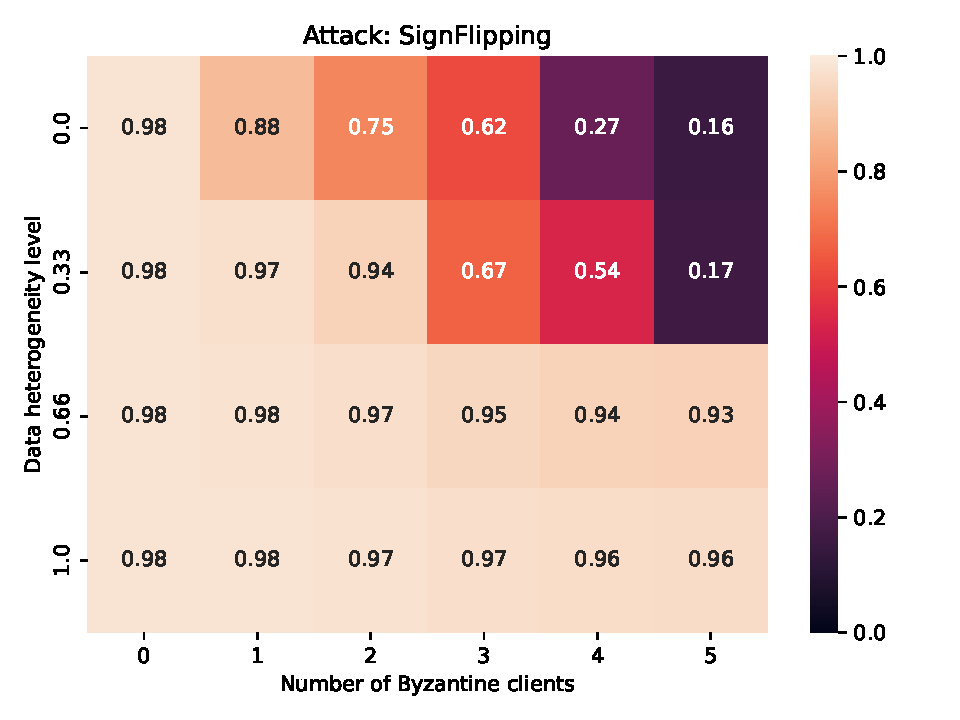
\includegraphics[width=\textwidth]{../plots/mnist_clipping_heatmaps/cnn_mnist_clipping_2/test_SignFlipping_mnist_cnn_mnist_clipping_2_gamma_similarity_niid_NNM_ARC_GeometricMedian_nb_honest_clients_10_tolerated_f_equal_real.pdf}
        \caption{Hardtanh $C{=}2$}
        \label{fig:gm_sf_hardtanh_2}
    \end{subfigure}
    \hfill
    \begin{subfigure}[b]{0.32\textwidth}
        \centering
        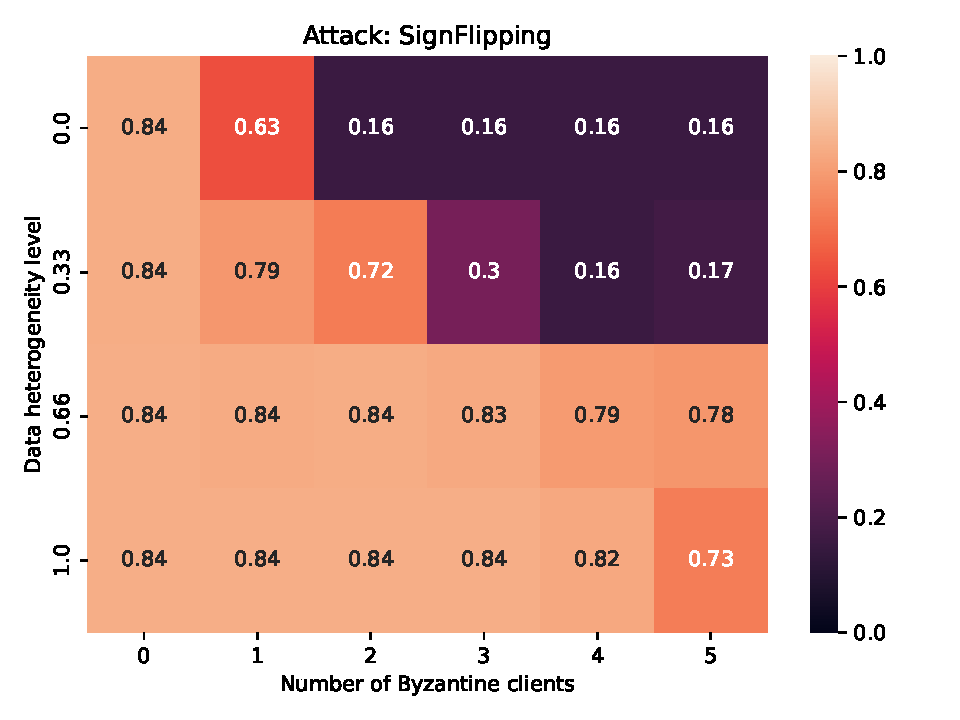
\includegraphics[width=\textwidth]{../activation_clip_plots/cnn_mnist_clip_ste_1/test_SignFlipping_mnist_cnn_mnist_clip_ste_1_gamma_similarity_niid_NNM_ARC_GeometricMedian_nb_honest_clients_10_tolerated_f_equal_real.pdf}
        \caption{STE $C{=}1$}
        \label{fig:gm_sf_ste_1}
    \end{subfigure}
    \vspace{0.3cm}
    \begin{subfigure}[b]{0.32\textwidth}
        \centering
        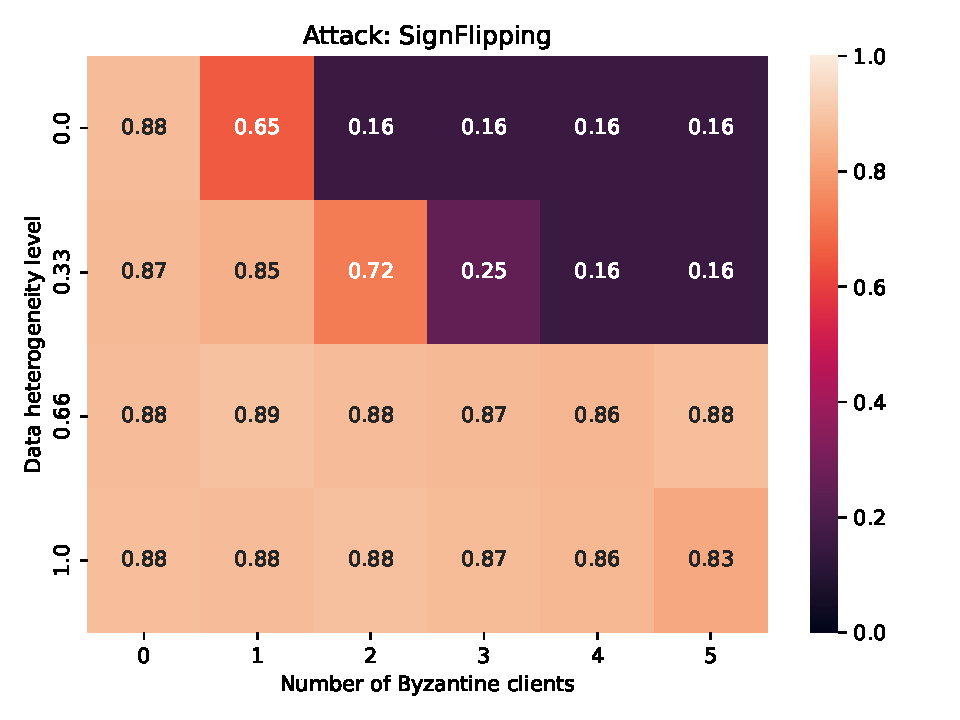
\includegraphics[width=\textwidth]{../activation_clip_plots/cnn_mnist_clip_ste_2/test_SignFlipping_mnist_cnn_mnist_clip_ste_2_gamma_similarity_niid_NNM_ARC_GeometricMedian_nb_honest_clients_10_tolerated_f_equal_real.pdf}
        \caption{STE $C{=}2$}
        \label{fig:gm_sf_ste_2}
    \end{subfigure}
    \hfill
    \begin{subfigure}[b]{0.32\textwidth}
        \centering
        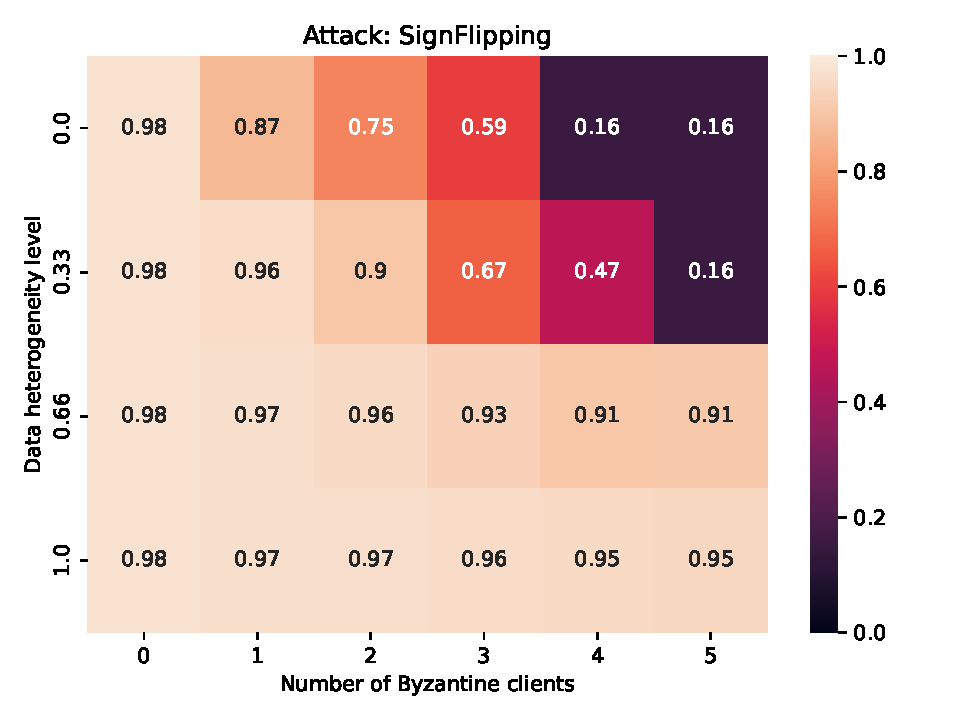
\includegraphics[width=\textwidth]{../activation_clip_plots/cnn_mnist_clip_ramp_1/test_SignFlipping_mnist_cnn_mnist_clip_ramp_1_gamma_similarity_niid_NNM_ARC_GeometricMedian_nb_honest_clients_10_tolerated_f_equal_real.pdf}
        \caption{Ramp $C{=}1$ ($r{=}2$)}
        \label{fig:gm_sf_ramp_1}
    \end{subfigure}
    \caption{Geometric Median (GM) under Sign Flipping Attack.}
    \label{fig:gm_sf_grid}
\end{figure}
\clearpage
\subsection{GM under IPM}
\begin{figure}[htbp]
    \centering
    \begin{subfigure}[b]{0.32\textwidth}
        \centering
        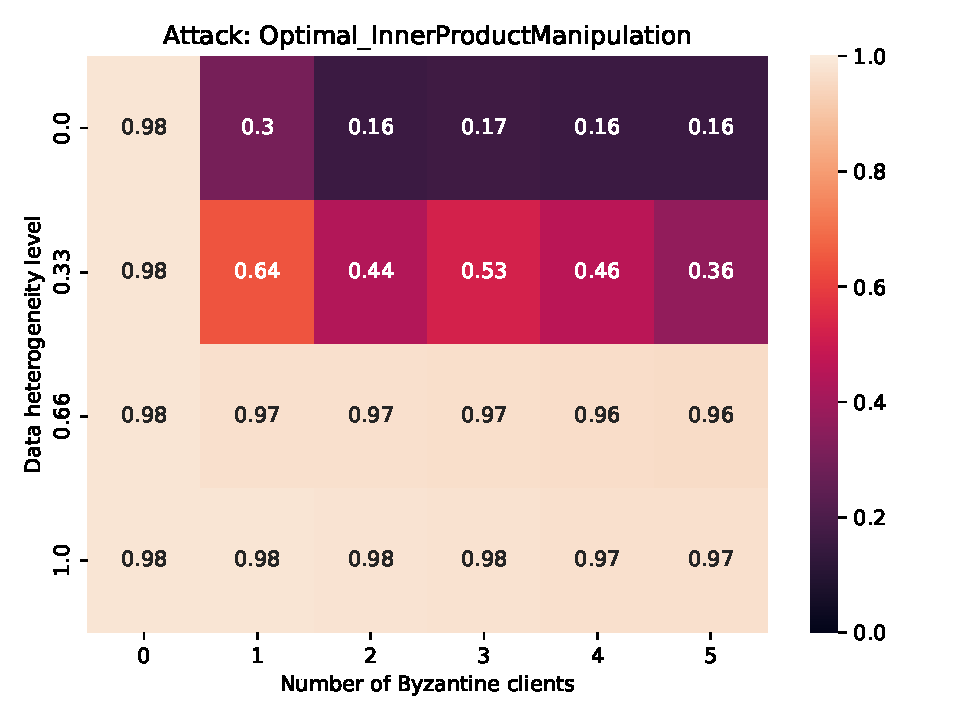
\includegraphics[width=\textwidth]{../plots/mnist_clipping_heatmaps/cnn_mnist/test_Optimal_InnerProductManipulation_mnist_cnn_mnist_gamma_similarity_niid_NNM_ARC_GeometricMedian_nb_honest_clients_10_tolerated_f_equal_real.pdf}
        \caption{No Clip (ReLU)}
        \label{fig:gm_ipm_noclip}
    \end{subfigure}
    \hfill
    \begin{subfigure}[b]{0.32\textwidth}
        \centering
        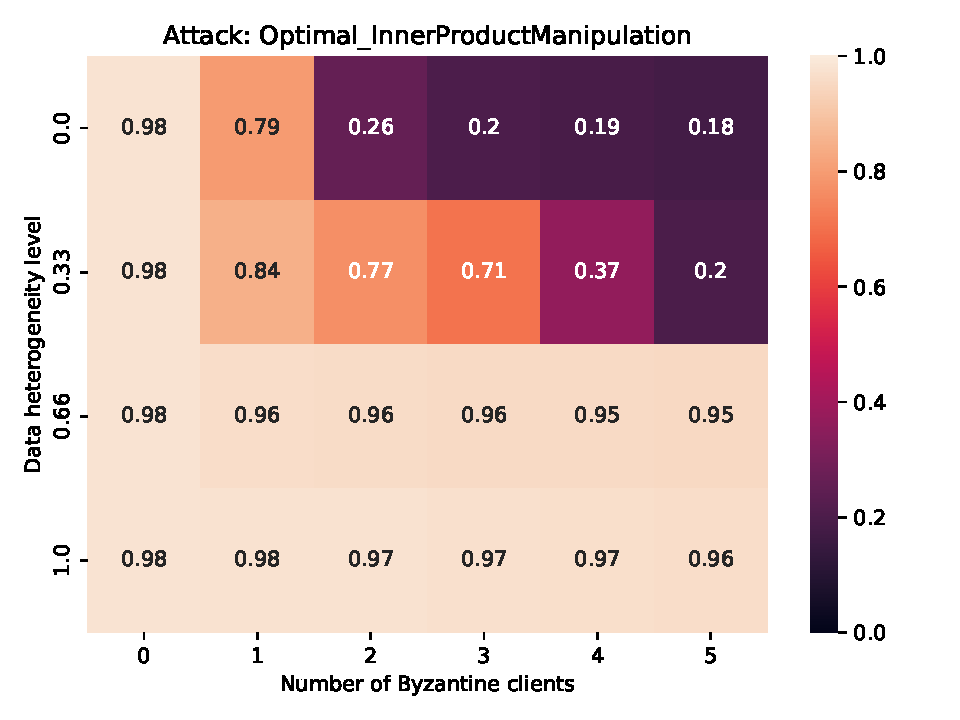
\includegraphics[width=\textwidth]{../plots/cnn_tanh_heatmaps/test_Optimal_InnerProductManipulation_mnist_cnn_mnist_tanh_gamma_similarity_niid_NNM_ARC_GeometricMedian_nb_honest_clients_10_tolerated_f_equal_real.pdf}
        \caption{Tanh}
        \label{fig:gm_ipm_tanh}
    \end{subfigure}
    \hfill
    \begin{subfigure}[b]{0.32\textwidth}
        \centering
        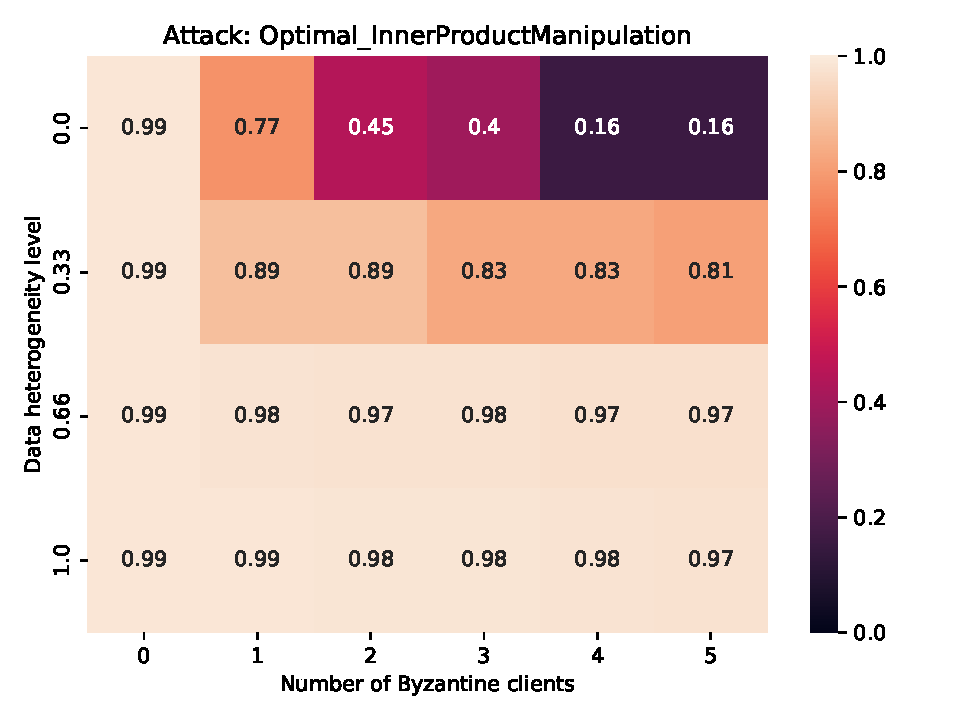
\includegraphics[width=\textwidth]{../plots/cnn_clipped_heatmaps/test_Optimal_InnerProductManipulation_mnist_cnn_mnist_gamma_similarity_niid_NNM_ARC_GeometricMedian_nb_honest_clients_10_tolerated_f_equal_real.pdf}
        \caption{Grad-Norm Clip $=21$}
        \label{fig:gm_ipm_gradnorm21}
    \end{subfigure}
    \vspace{0.3cm}
    \begin{subfigure}[b]{0.32\textwidth}
        \centering
        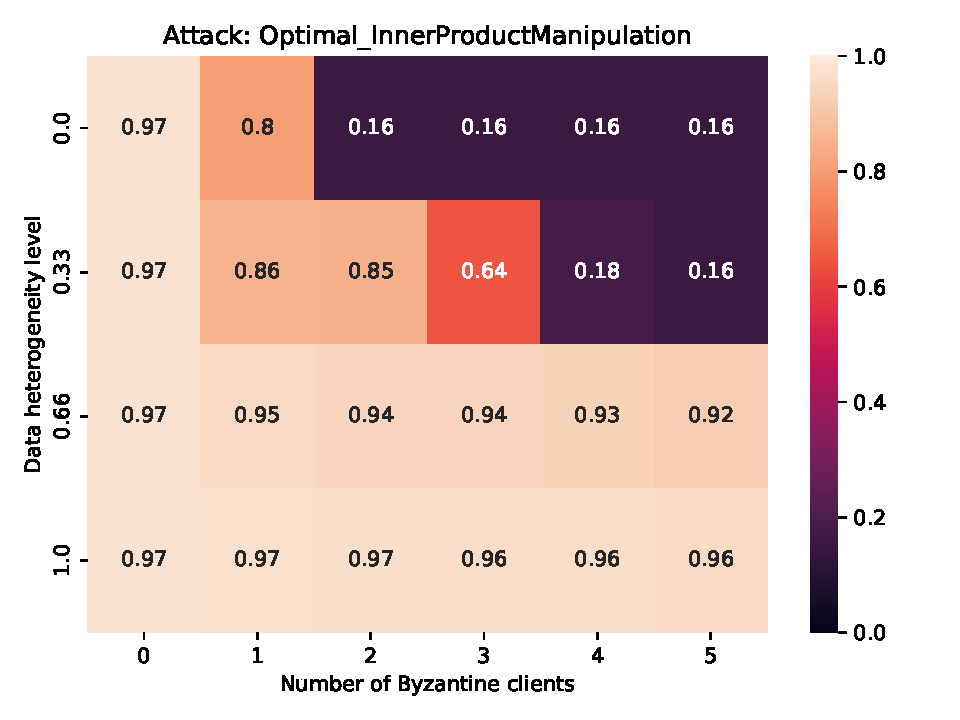
\includegraphics[width=\textwidth]{../plots/mnist_clipping_heatmaps/cnn_mnist_clipping_1/test_Optimal_InnerProductManipulation_mnist_cnn_mnist_clipping_1_gamma_similarity_niid_NNM_ARC_GeometricMedian_nb_honest_clients_10_tolerated_f_equal_real.pdf}
        \caption{Hardtanh $C{=}1$}
        \label{fig:gm_ipm_hardtanh_1}
    \end{subfigure}
    \hfill
    \begin{subfigure}[b]{0.32\textwidth}
        \centering
        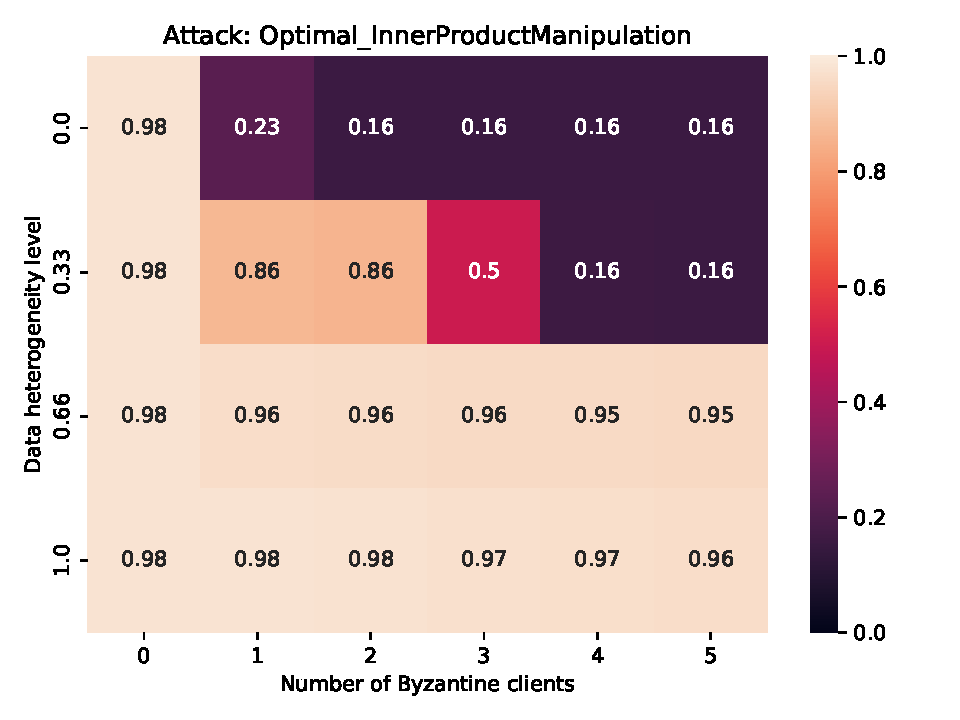
\includegraphics[width=\textwidth]{../plots/mnist_clipping_heatmaps/cnn_mnist_clipping_2/test_Optimal_InnerProductManipulation_mnist_cnn_mnist_clipping_2_gamma_similarity_niid_NNM_ARC_GeometricMedian_nb_honest_clients_10_tolerated_f_equal_real.pdf}
        \caption{Hardtanh $C{=}2$}
        \label{fig:gm_ipm_hardtanh_2}
    \end{subfigure}
    \hfill
    \begin{subfigure}[b]{0.32\textwidth}
        \centering
        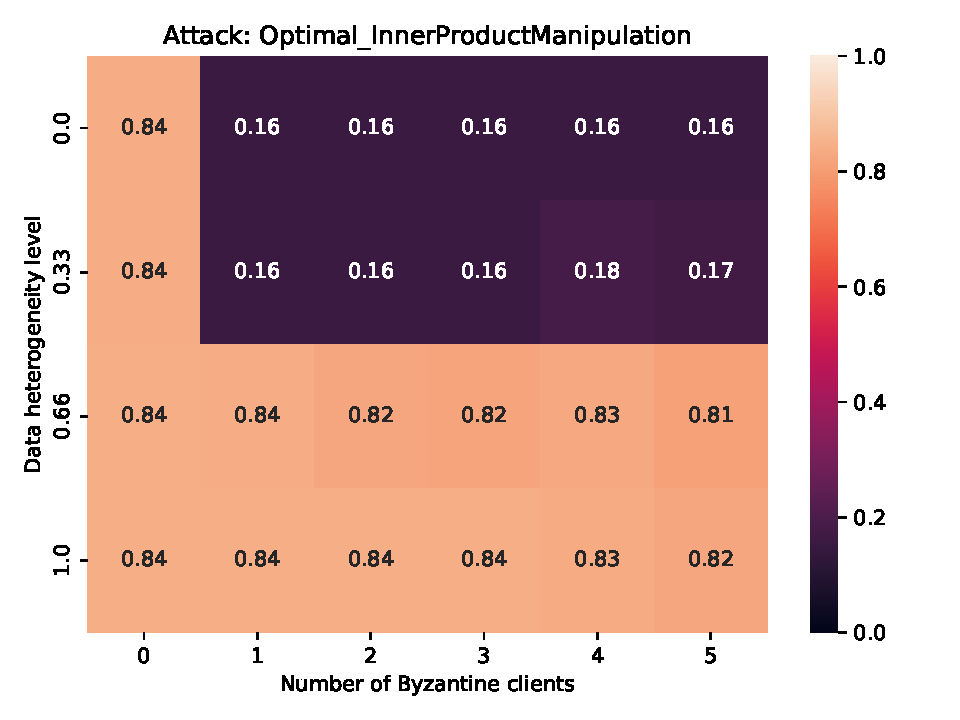
\includegraphics[width=\textwidth]{../activation_clip_plots/cnn_mnist_clip_ste_1/test_Optimal_InnerProductManipulation_mnist_cnn_mnist_clip_ste_1_gamma_similarity_niid_NNM_ARC_GeometricMedian_nb_honest_clients_10_tolerated_f_equal_real.pdf}
        \caption{STE $C{=}1$}
        \label{fig:gm_ipm_ste_1}
    \end{subfigure}
    \vspace{0.3cm}
    \begin{subfigure}[b]{0.32\textwidth}
        \centering
        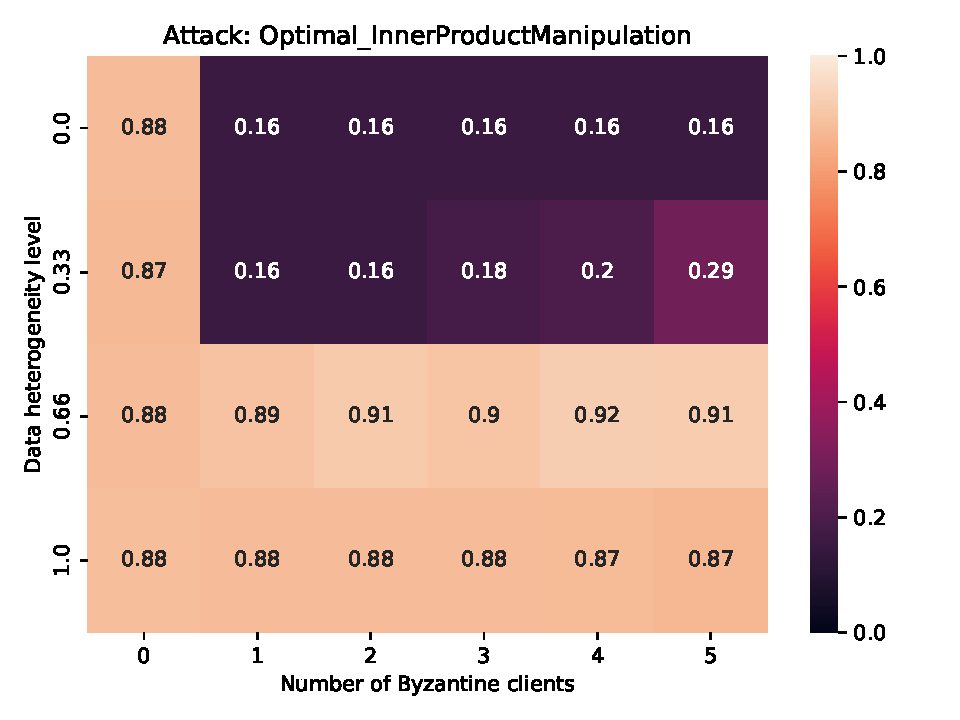
\includegraphics[width=\textwidth]{../activation_clip_plots/cnn_mnist_clip_ste_2/test_Optimal_InnerProductManipulation_mnist_cnn_mnist_clip_ste_2_gamma_similarity_niid_NNM_ARC_GeometricMedian_nb_honest_clients_10_tolerated_f_equal_real.pdf}
        \caption{STE $C{=}2$}
        \label{fig:gm_ipm_ste_2}
    \end{subfigure}
    \hfill
    \begin{subfigure}[b]{0.32\textwidth}
        \centering
        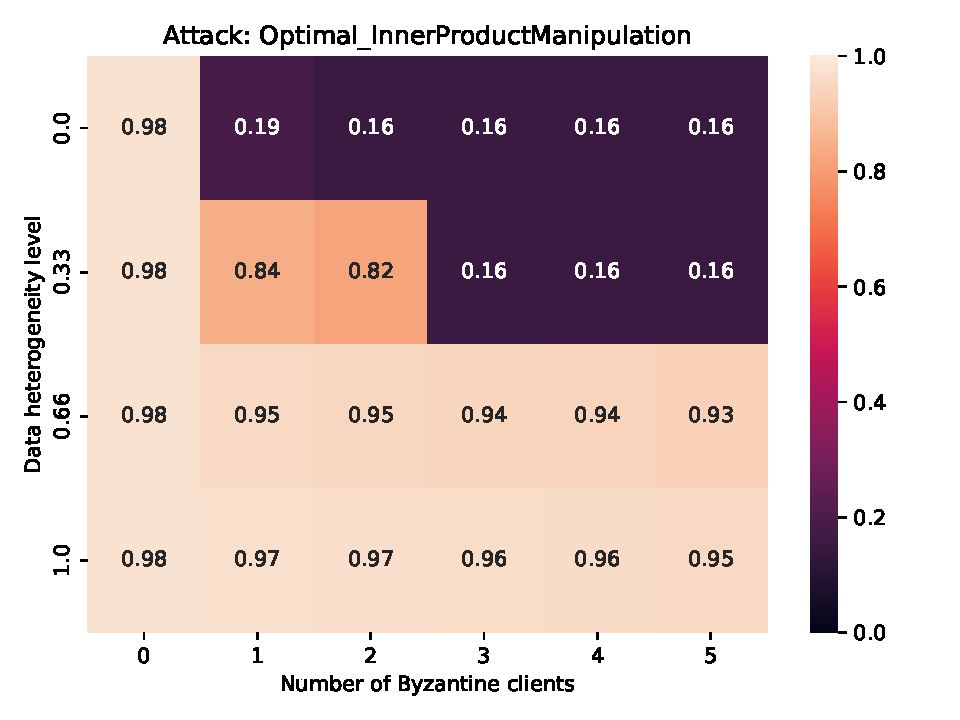
\includegraphics[width=\textwidth]{../activation_clip_plots/cnn_mnist_clip_ramp_1/test_Optimal_InnerProductManipulation_mnist_cnn_mnist_clip_ramp_1_gamma_similarity_niid_NNM_ARC_GeometricMedian_nb_honest_clients_10_tolerated_f_equal_real.pdf}
        \caption{Ramp $C{=}1$ ($r{=}2$)}
        \label{fig:gm_ipm_ramp_1}
    \end{subfigure}
    \caption{Geometric Median (GM) under Optimal IPM Attack.}
    \label{fig:gm_ipm_grid}
\end{figure}
\clearpage
\section{Multi-Krum (MK)}
\subsection{MK under Worst-Case across all Attacks}
\begin{figure}[htbp]
    \centering
    \begin{subfigure}[b]{0.32\textwidth}
        \centering
        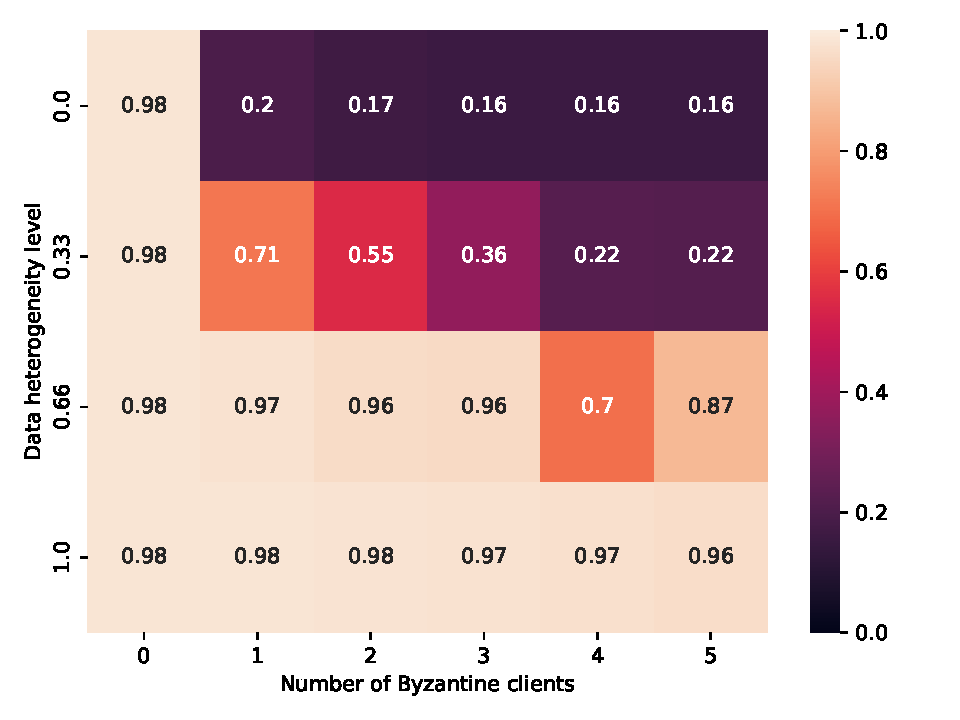
\includegraphics[width=\textwidth]{../plots/mnist_clipping_heatmaps/cnn_mnist/test_mnist_cnn_mnist_gamma_similarity_niid_NNM_ARC_MultiKrum_nb_honest_clients_10_tolerated_f_equal_real.pdf}
        \caption{No Clip (ReLU)}
        \label{fig:mk_worst_case_noclip}
    \end{subfigure}
    \hfill
    \begin{subfigure}[b]{0.32\textwidth}
        \centering
        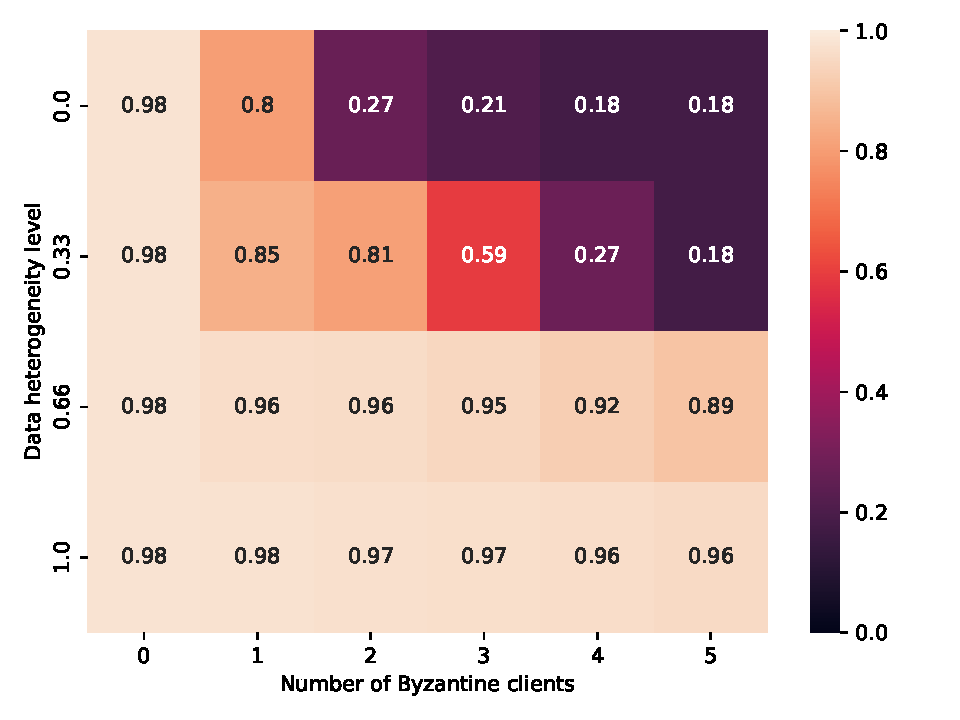
\includegraphics[width=\textwidth]{../plots/cnn_tanh_heatmaps/test_mnist_cnn_mnist_tanh_gamma_similarity_niid_NNM_ARC_MultiKrum_nb_honest_clients_10_tolerated_f_equal_real.pdf}
        \caption{Tanh}
        \label{fig:mk_worst_case_tanh}
    \end{subfigure}
    \hfill
    \begin{subfigure}[b]{0.32\textwidth}
        \centering
        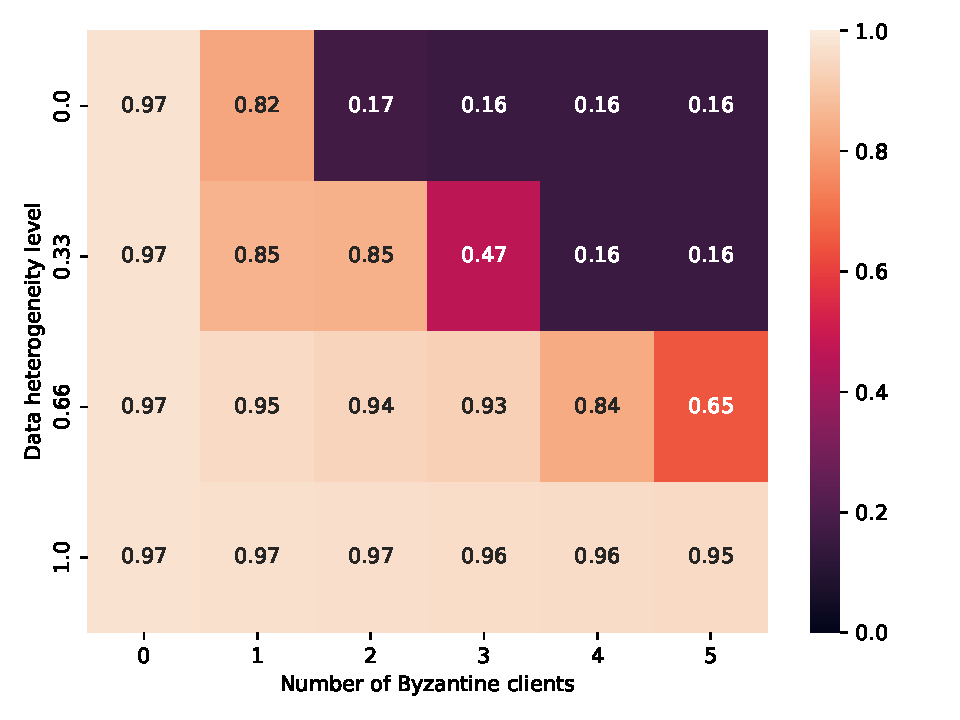
\includegraphics[width=\textwidth]{../plots/mnist_clipping_heatmaps/cnn_mnist_clipping_1/test_mnist_cnn_mnist_clipping_1_gamma_similarity_niid_NNM_ARC_MultiKrum_nb_honest_clients_10_tolerated_f_equal_real.pdf}
        \caption{Hardtanh $C{=}1$}
        \label{fig:mk_worst_case_hardtanh_1}
    \end{subfigure}
    \vspace{0.3cm}
    \begin{subfigure}[b]{0.32\textwidth}
        \centering
        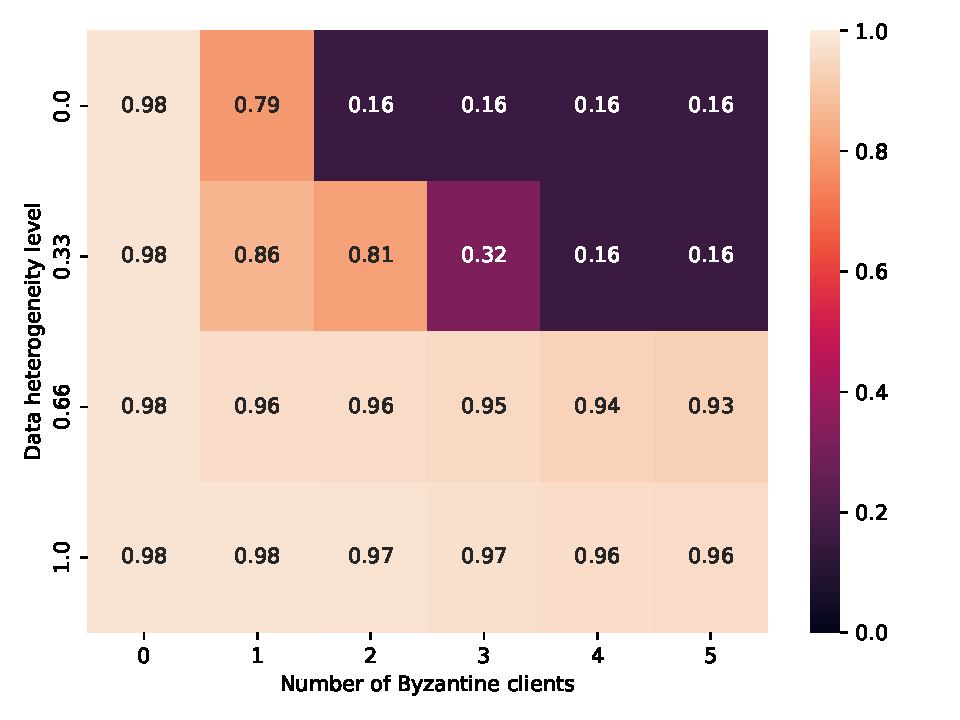
\includegraphics[width=\textwidth]{../plots/mnist_clipping_heatmaps/cnn_mnist_clipping_2/test_mnist_cnn_mnist_clipping_2_gamma_similarity_niid_NNM_ARC_MultiKrum_nb_honest_clients_10_tolerated_f_equal_real.pdf}
        \caption{Hardtanh $C{=}2$}
        \label{fig:mk_worst_case_hardtanh_2}
    \end{subfigure}
    \hfill
    \begin{subfigure}[b]{0.32\textwidth}
        \centering
        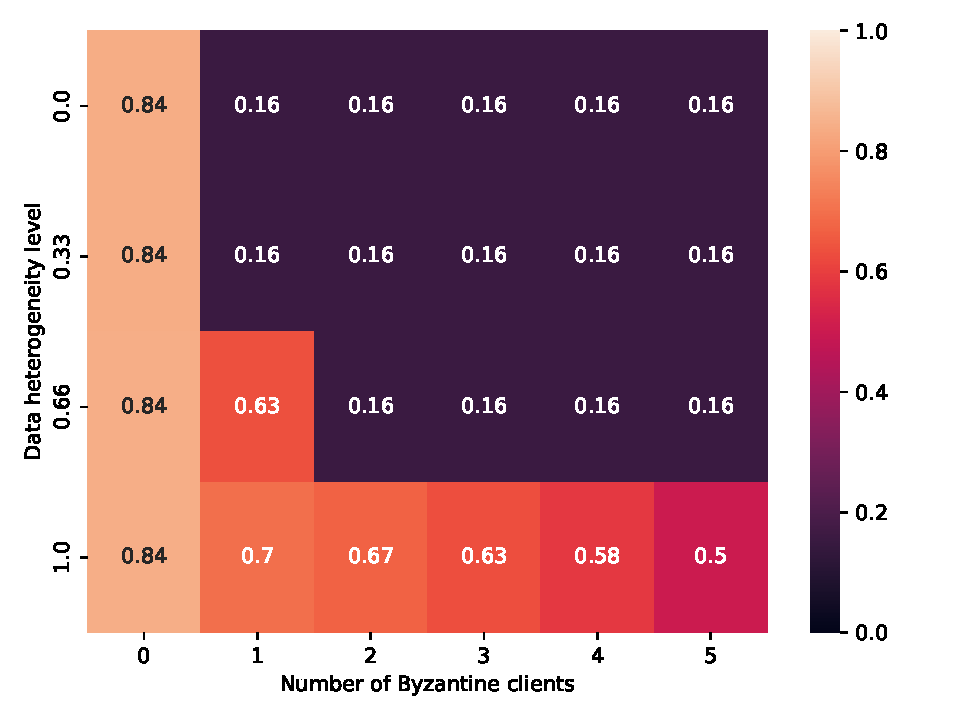
\includegraphics[width=\textwidth]{../activation_clip_plots/cnn_mnist_clip_ste_1/test_mnist_cnn_mnist_clip_ste_1_gamma_similarity_niid_NNM_ARC_MultiKrum_nb_honest_clients_10_tolerated_f_equal_real.pdf}
        \caption{STE $C{=}1$}
        \label{fig:mk_worst_case_ste_1}
    \end{subfigure}
    \hfill
    \begin{subfigure}[b]{0.32\textwidth}
        \centering
        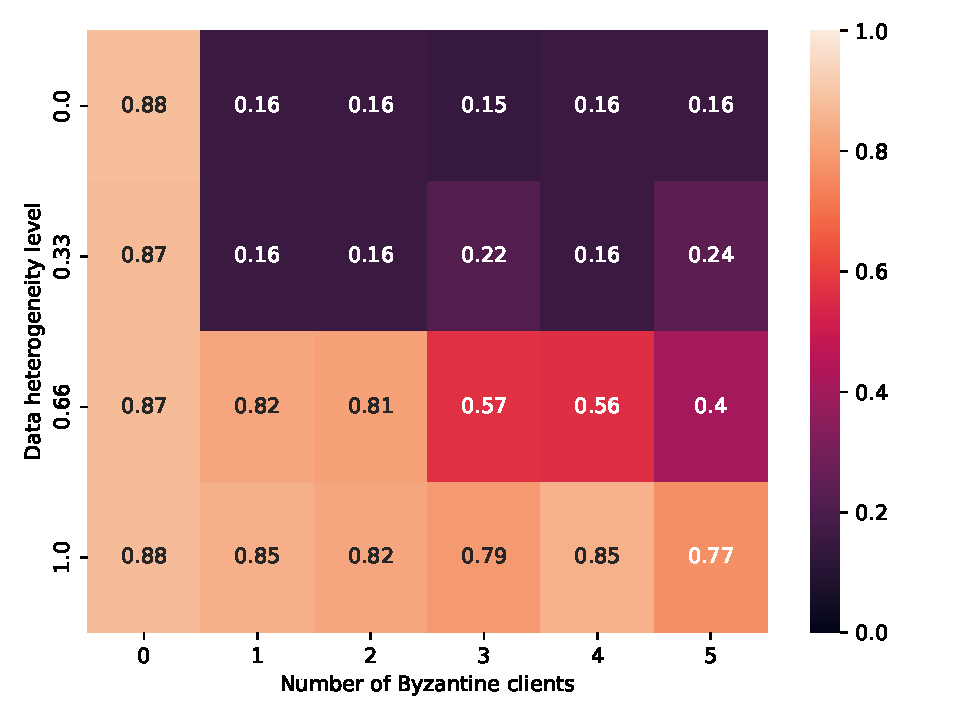
\includegraphics[width=\textwidth]{../activation_clip_plots/cnn_mnist_clip_ste_2/test_mnist_cnn_mnist_clip_ste_2_gamma_similarity_niid_NNM_ARC_MultiKrum_nb_honest_clients_10_tolerated_f_equal_real.pdf}
        \caption{STE $C{=}2$}
        \label{fig:mk_worst_case_ste_2}
    \end{subfigure}
    \vspace{0.3cm}
    \begin{subfigure}[b]{0.32\textwidth}
        \centering
        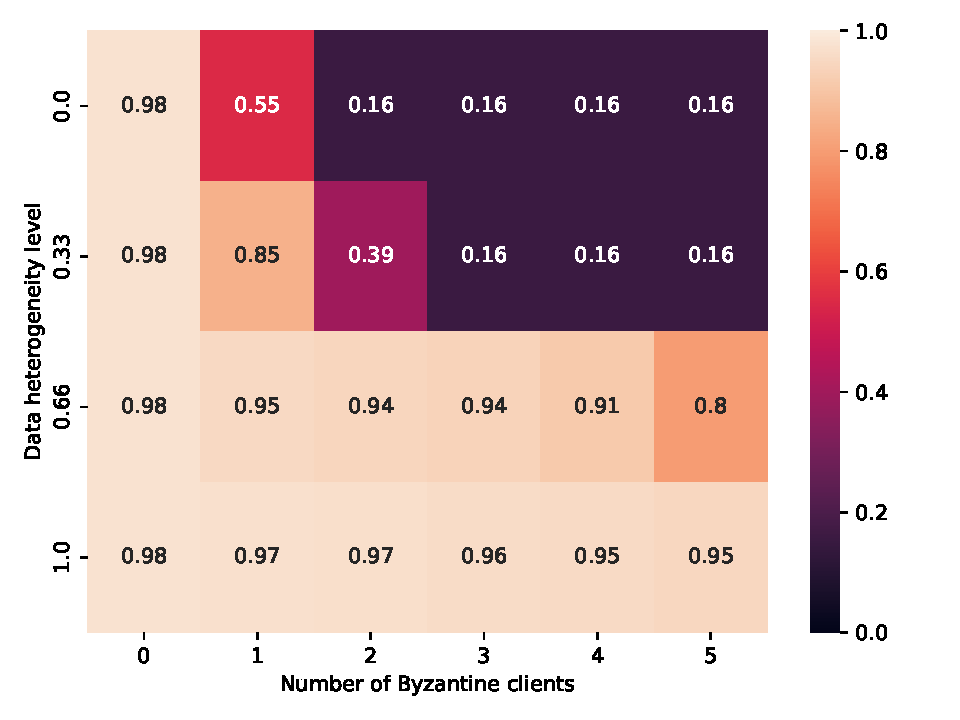
\includegraphics[width=\textwidth]{../activation_clip_plots/cnn_mnist_clip_ramp_1/test_mnist_cnn_mnist_clip_ramp_1_gamma_similarity_niid_NNM_ARC_MultiKrum_nb_honest_clients_10_tolerated_f_equal_real.pdf}
        \caption{Ramp $C{=}1$ ($r{=}2$)}
        \label{fig:mk_worst_case_ramp_1}
    \end{subfigure}
    \caption{Multi-Krum (MK) under Worst-Case across all Attacks.}
    \label{fig:mk_worst_case_grid}
\end{figure}
\clearpage
\subsection{MK under ALIE}
\begin{figure}[htbp]
    \centering
    \begin{subfigure}[b]{0.32\textwidth}
        \centering
        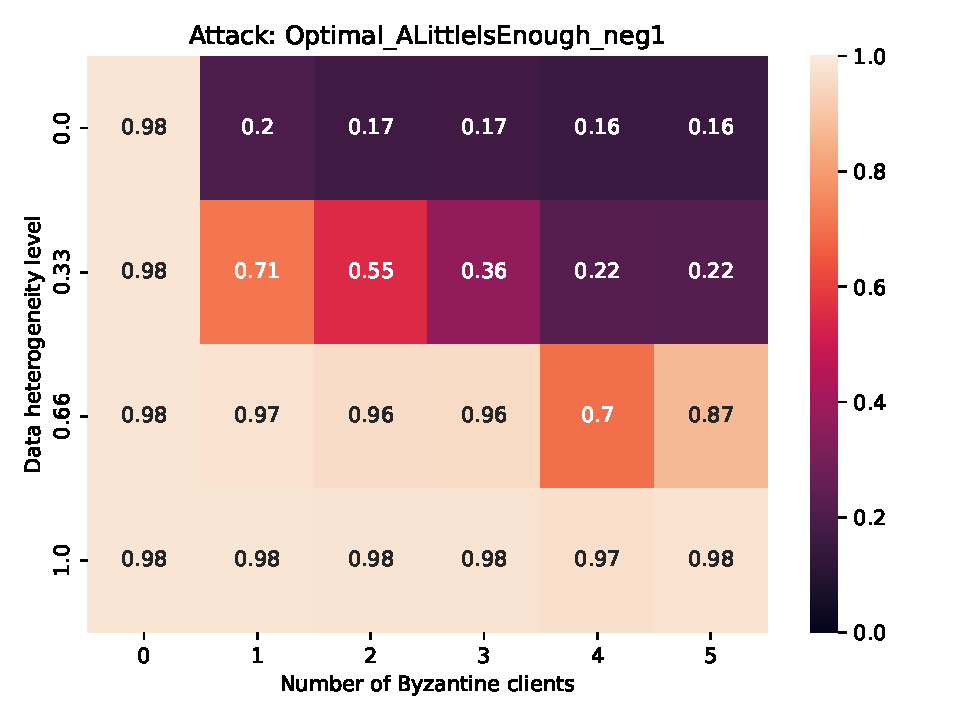
\includegraphics[width=\textwidth]{../plots/mnist_clipping_heatmaps/cnn_mnist/test_Optimal_ALittleIsEnough_neg1_mnist_cnn_mnist_gamma_similarity_niid_NNM_ARC_MultiKrum_nb_honest_clients_10_tolerated_f_equal_real.pdf}
        \caption{No Clip (ReLU)}
        \label{fig:mk_alie_noclip}
    \end{subfigure}
    \hfill
    \begin{subfigure}[b]{0.32\textwidth}
        \centering
        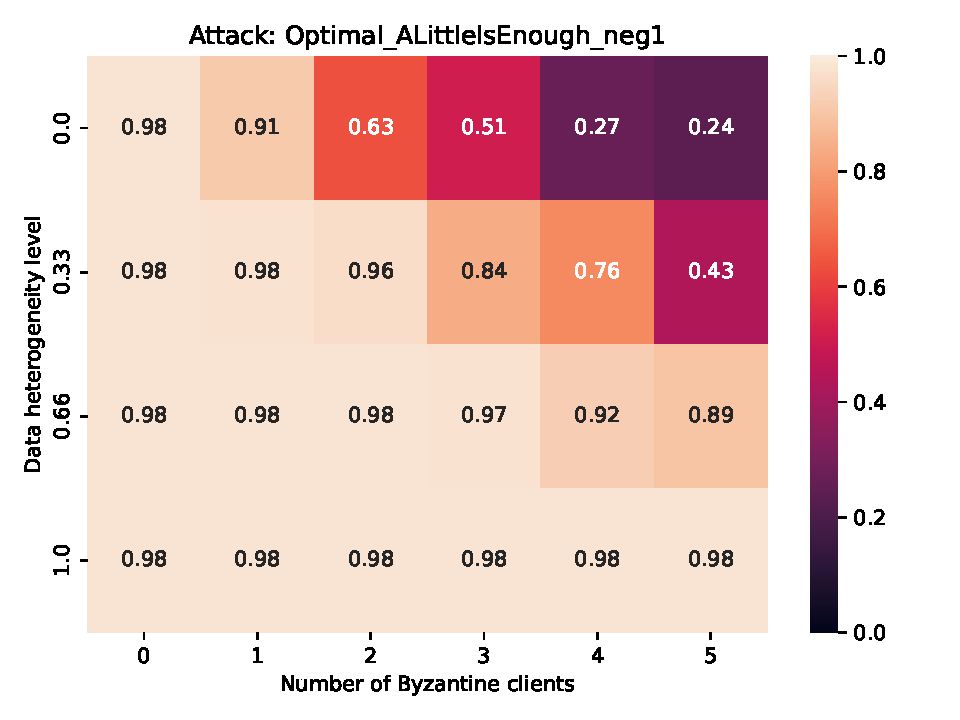
\includegraphics[width=\textwidth]{../plots/cnn_tanh_heatmaps/test_Optimal_ALittleIsEnough_neg1_mnist_cnn_mnist_tanh_gamma_similarity_niid_NNM_ARC_MultiKrum_nb_honest_clients_10_tolerated_f_equal_real.pdf}
        \caption{Tanh}
        \label{fig:mk_alie_tanh}
    \end{subfigure}
    \hfill
    \begin{subfigure}[b]{0.32\textwidth}
        \centering
        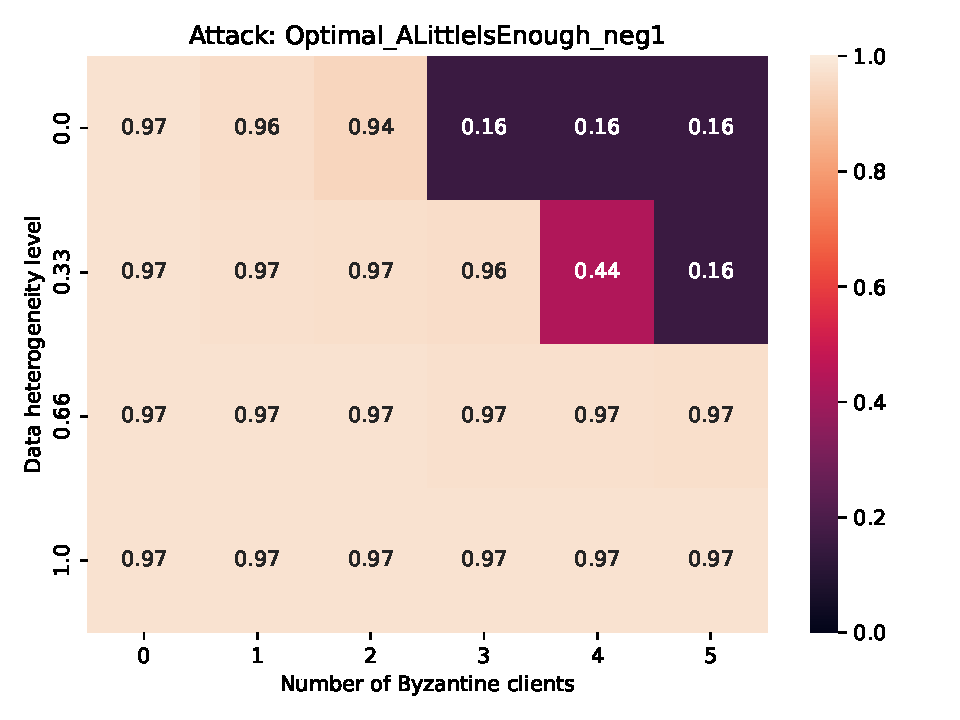
\includegraphics[width=\textwidth]{../plots/mnist_clipping_heatmaps/cnn_mnist_clipping_1/test_Optimal_ALittleIsEnough_neg1_mnist_cnn_mnist_clipping_1_gamma_similarity_niid_NNM_ARC_MultiKrum_nb_honest_clients_10_tolerated_f_equal_real.pdf}
        \caption{Hardtanh $C{=}1$}
        \label{fig:mk_alie_hardtanh_1}
    \end{subfigure}
    \vspace{0.3cm}
    \begin{subfigure}[b]{0.32\textwidth}
        \centering
        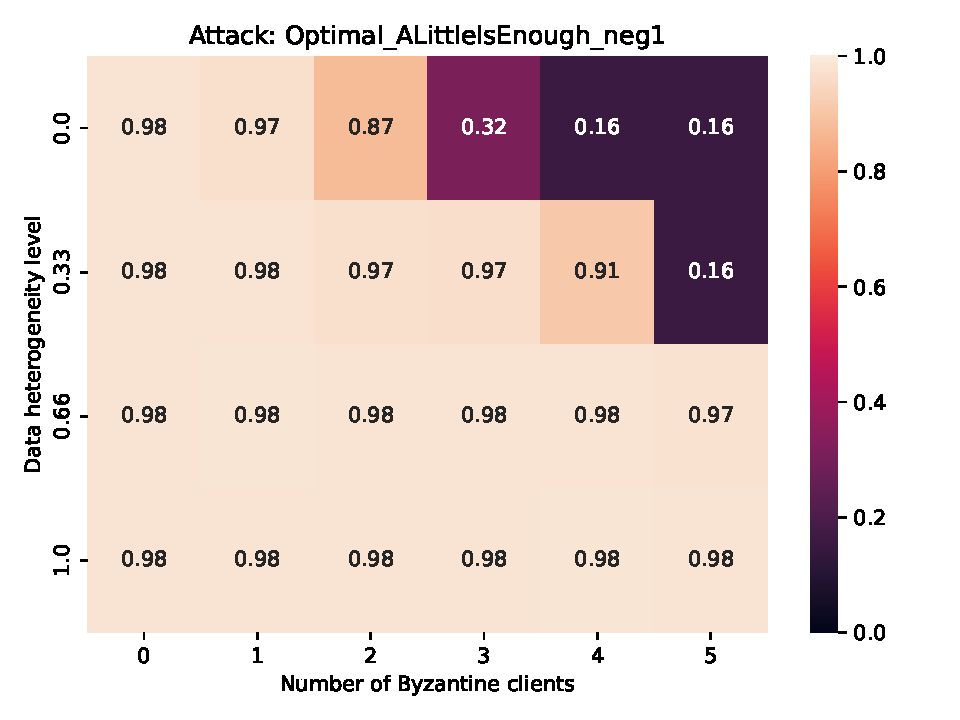
\includegraphics[width=\textwidth]{../plots/mnist_clipping_heatmaps/cnn_mnist_clipping_2/test_Optimal_ALittleIsEnough_neg1_mnist_cnn_mnist_clipping_2_gamma_similarity_niid_NNM_ARC_MultiKrum_nb_honest_clients_10_tolerated_f_equal_real.pdf}
        \caption{Hardtanh $C{=}2$}
        \label{fig:mk_alie_hardtanh_2}
    \end{subfigure}
    \hfill
    \begin{subfigure}[b]{0.32\textwidth}
        \centering
        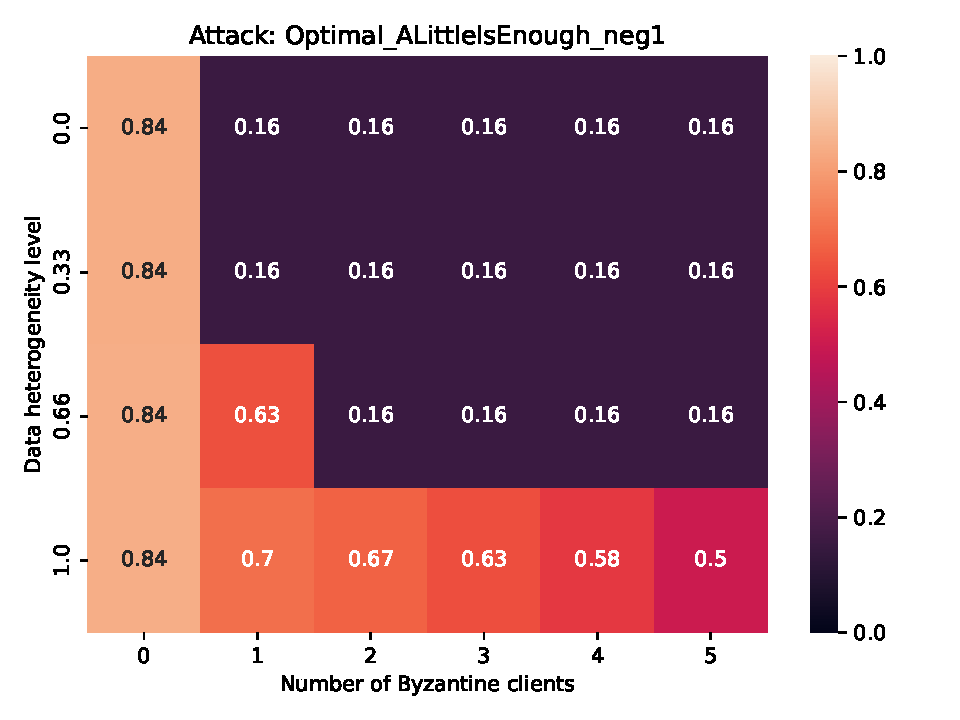
\includegraphics[width=\textwidth]{../activation_clip_plots/cnn_mnist_clip_ste_1/test_Optimal_ALittleIsEnough_neg1_mnist_cnn_mnist_clip_ste_1_gamma_similarity_niid_NNM_ARC_MultiKrum_nb_honest_clients_10_tolerated_f_equal_real.pdf}
        \caption{STE $C{=}1$}
        \label{fig:mk_alie_ste_1}
    \end{subfigure}
    \hfill
    \begin{subfigure}[b]{0.32\textwidth}
        \centering
        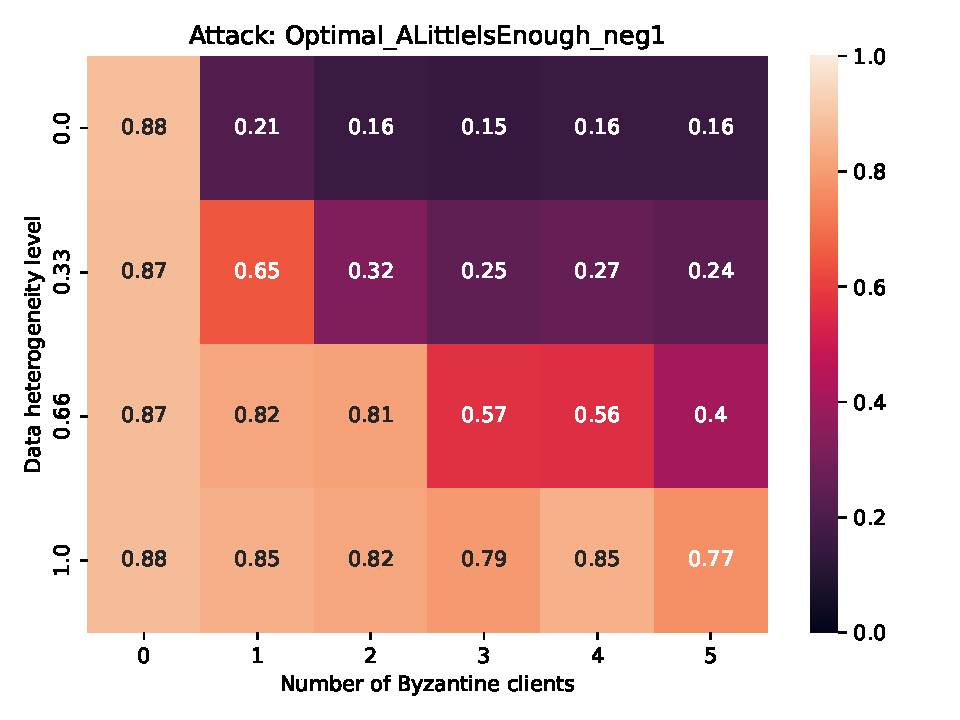
\includegraphics[width=\textwidth]{../activation_clip_plots/cnn_mnist_clip_ste_2/test_Optimal_ALittleIsEnough_neg1_mnist_cnn_mnist_clip_ste_2_gamma_similarity_niid_NNM_ARC_MultiKrum_nb_honest_clients_10_tolerated_f_equal_real.pdf}
        \caption{STE $C{=}2$}
        \label{fig:mk_alie_ste_2}
    \end{subfigure}
    \vspace{0.3cm}
    \begin{subfigure}[b]{0.32\textwidth}
        \centering
        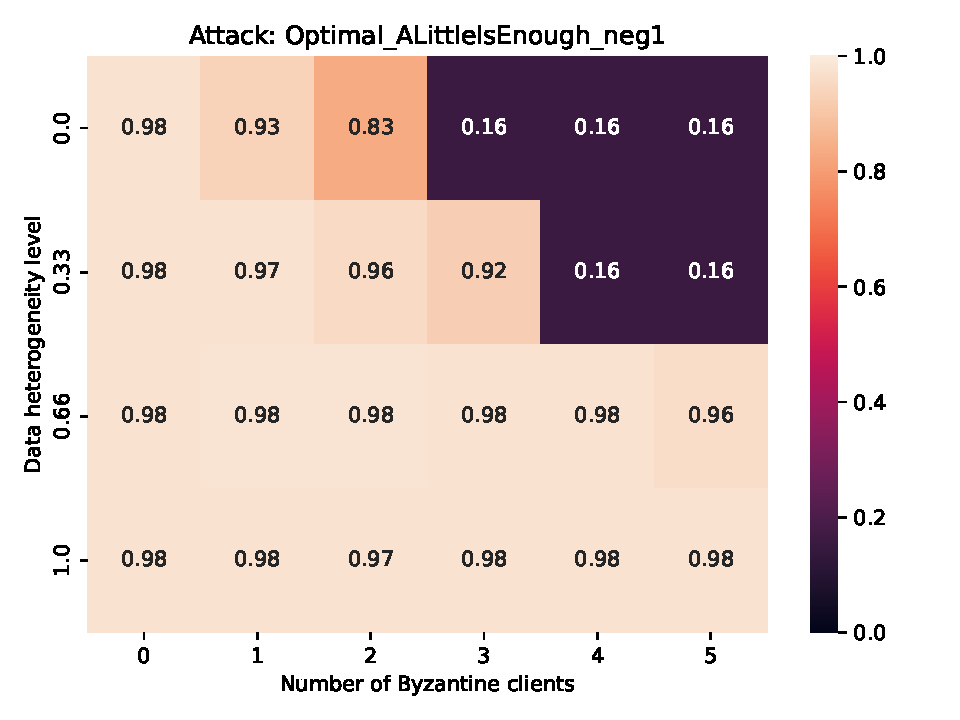
\includegraphics[width=\textwidth]{../activation_clip_plots/cnn_mnist_clip_ramp_1/test_Optimal_ALittleIsEnough_neg1_mnist_cnn_mnist_clip_ramp_1_gamma_similarity_niid_NNM_ARC_MultiKrum_nb_honest_clients_10_tolerated_f_equal_real.pdf}
        \caption{Ramp $C{=}1$ ($r{=}2$)}
        \label{fig:mk_alie_ramp_1}
    \end{subfigure}
    \caption{Multi-Krum (MK) under Optimal ALIE Attack.}
    \label{fig:mk_alie_grid}
\end{figure}
\clearpage
\subsection{MK under SF}
\begin{figure}[htbp]
    \centering
    \begin{subfigure}[b]{0.32\textwidth}
        \centering
        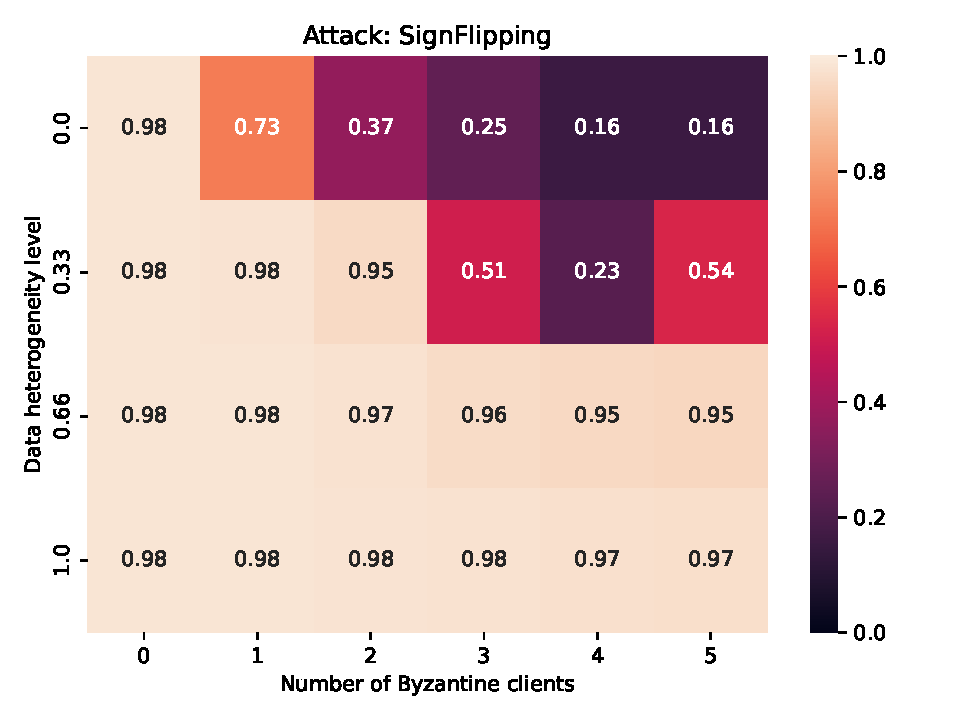
\includegraphics[width=\textwidth]{../plots/mnist_clipping_heatmaps/cnn_mnist/test_SignFlipping_mnist_cnn_mnist_gamma_similarity_niid_NNM_ARC_MultiKrum_nb_honest_clients_10_tolerated_f_equal_real.pdf}
        \caption{No Clip (ReLU)}
        \label{fig:mk_sf_noclip}
    \end{subfigure}
    \hfill
    \begin{subfigure}[b]{0.32\textwidth}
        \centering
        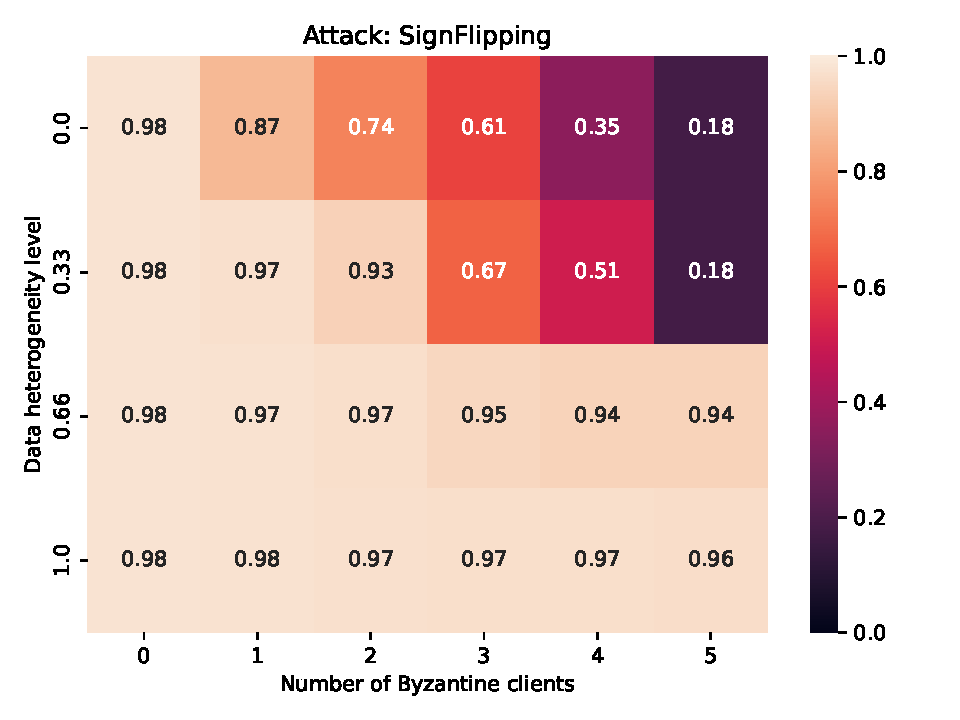
\includegraphics[width=\textwidth]{../plots/cnn_tanh_heatmaps/test_SignFlipping_mnist_cnn_mnist_tanh_gamma_similarity_niid_NNM_ARC_MultiKrum_nb_honest_clients_10_tolerated_f_equal_real.pdf}
        \caption{Tanh}
        \label{fig:mk_sf_tanh}
    \end{subfigure}
    \hfill
    \begin{subfigure}[b]{0.32\textwidth}
        \centering
        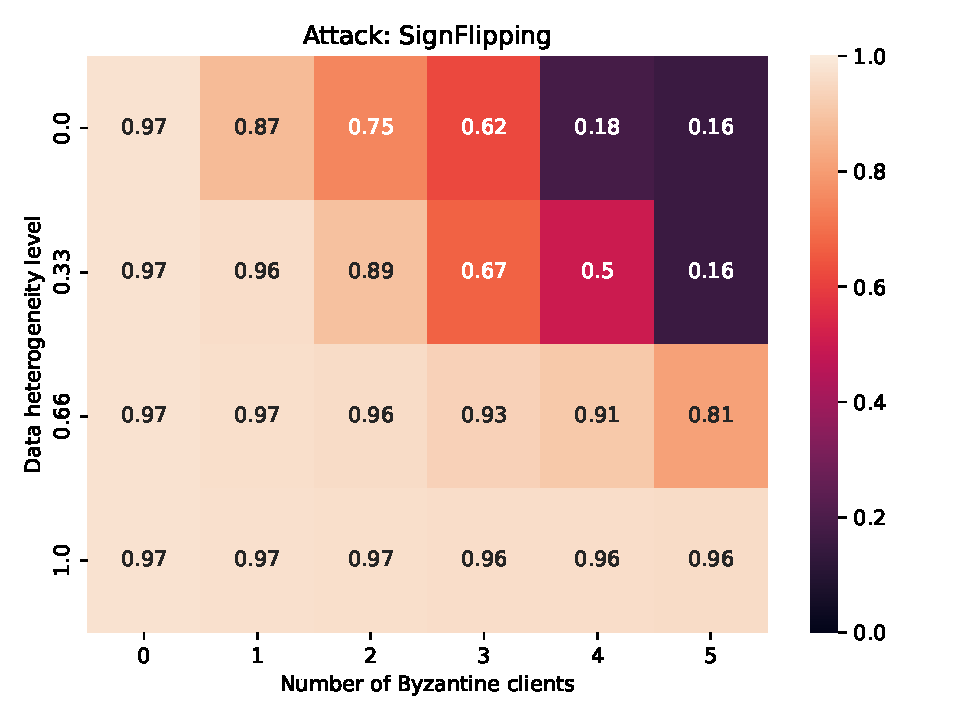
\includegraphics[width=\textwidth]{../plots/mnist_clipping_heatmaps/cnn_mnist_clipping_1/test_SignFlipping_mnist_cnn_mnist_clipping_1_gamma_similarity_niid_NNM_ARC_MultiKrum_nb_honest_clients_10_tolerated_f_equal_real.pdf}
        \caption{Hardtanh $C{=}1$}
        \label{fig:mk_sf_hardtanh_1}
    \end{subfigure}
    \vspace{0.3cm}
    \begin{subfigure}[b]{0.32\textwidth}
        \centering
        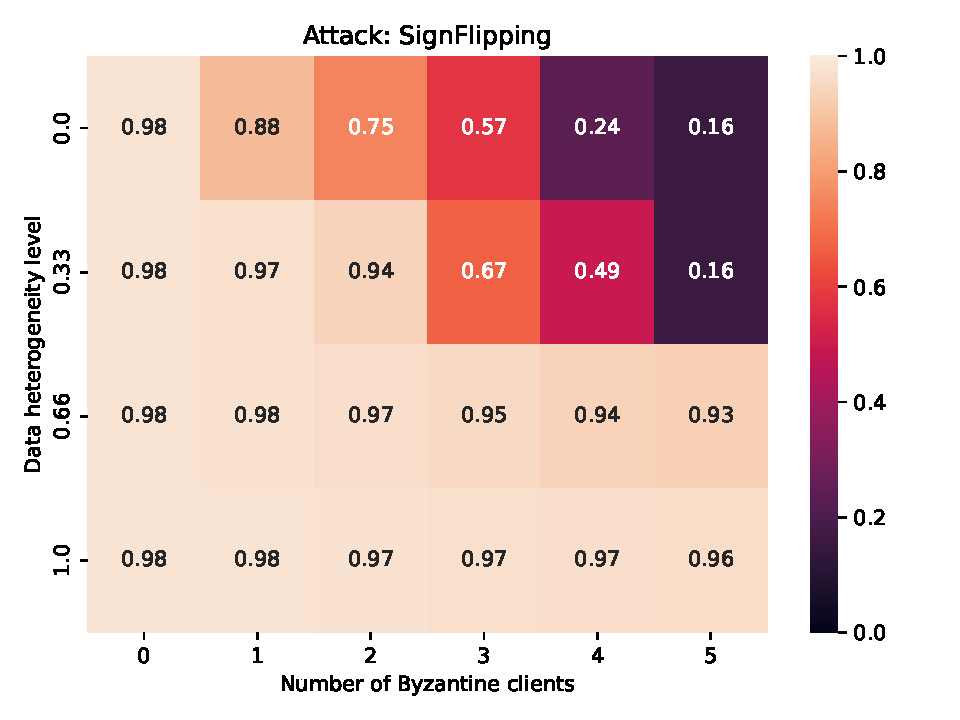
\includegraphics[width=\textwidth]{../plots/mnist_clipping_heatmaps/cnn_mnist_clipping_2/test_SignFlipping_mnist_cnn_mnist_clipping_2_gamma_similarity_niid_NNM_ARC_MultiKrum_nb_honest_clients_10_tolerated_f_equal_real.pdf}
        \caption{Hardtanh $C{=}2$}
        \label{fig:mk_sf_hardtanh_2}
    \end{subfigure}
    \hfill
    \begin{subfigure}[b]{0.32\textwidth}
        \centering
        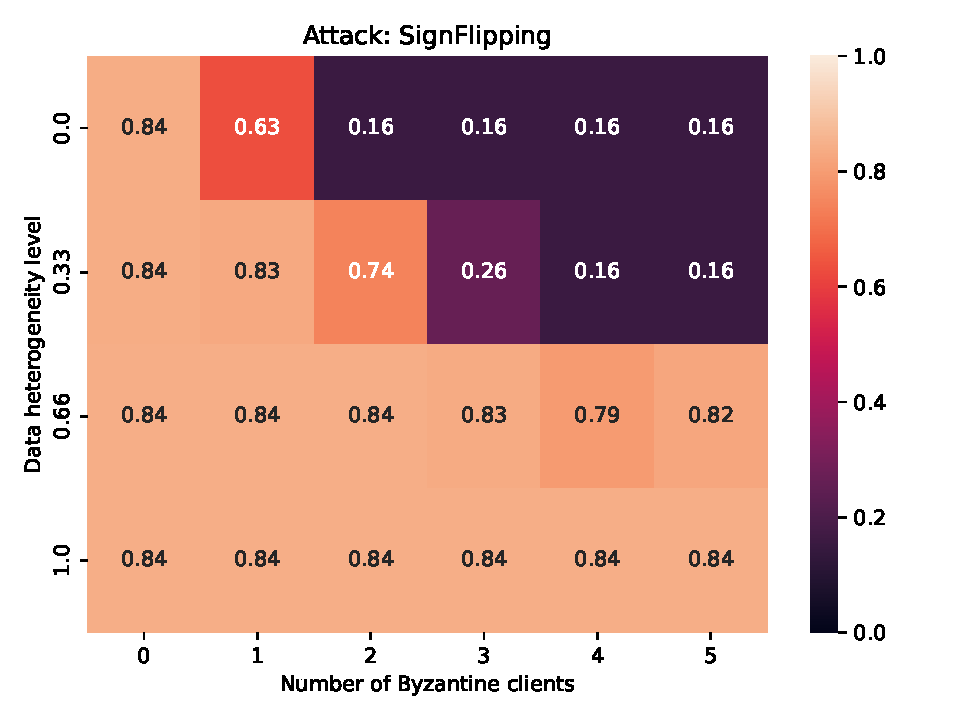
\includegraphics[width=\textwidth]{../activation_clip_plots/cnn_mnist_clip_ste_1/test_SignFlipping_mnist_cnn_mnist_clip_ste_1_gamma_similarity_niid_NNM_ARC_MultiKrum_nb_honest_clients_10_tolerated_f_equal_real.pdf}
        \caption{STE $C{=}1$}
        \label{fig:mk_sf_ste_1}
    \end{subfigure}
    \hfill
    \begin{subfigure}[b]{0.32\textwidth}
        \centering
        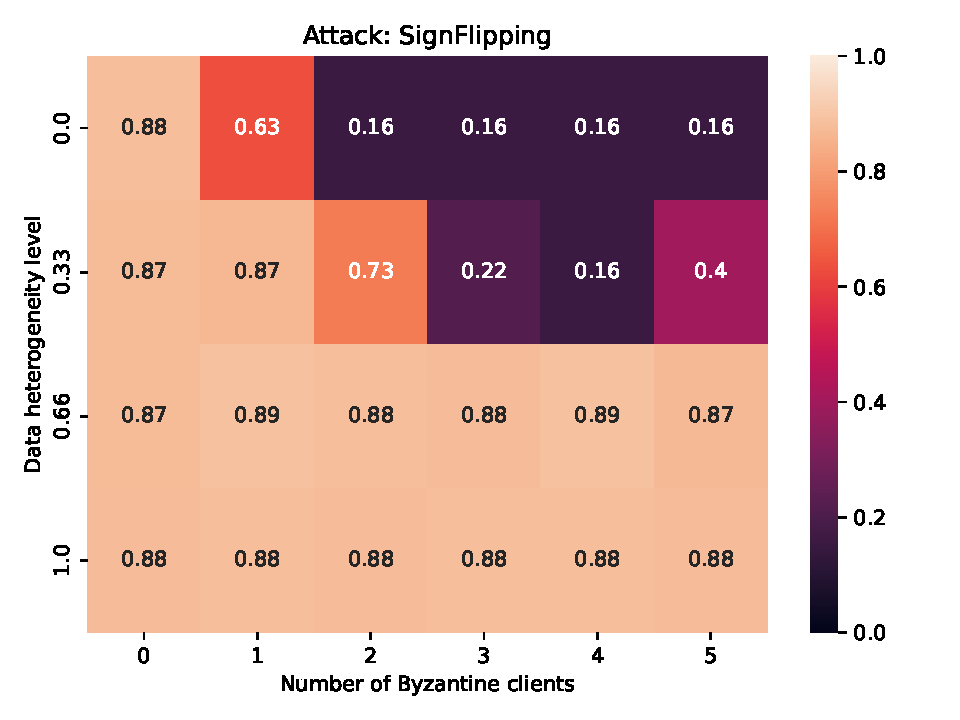
\includegraphics[width=\textwidth]{../activation_clip_plots/cnn_mnist_clip_ste_2/test_SignFlipping_mnist_cnn_mnist_clip_ste_2_gamma_similarity_niid_NNM_ARC_MultiKrum_nb_honest_clients_10_tolerated_f_equal_real.pdf}
        \caption{STE $C{=}2$}
        \label{fig:mk_sf_ste_2}
    \end{subfigure}
    \vspace{0.3cm}
    \begin{subfigure}[b]{0.32\textwidth}
        \centering
        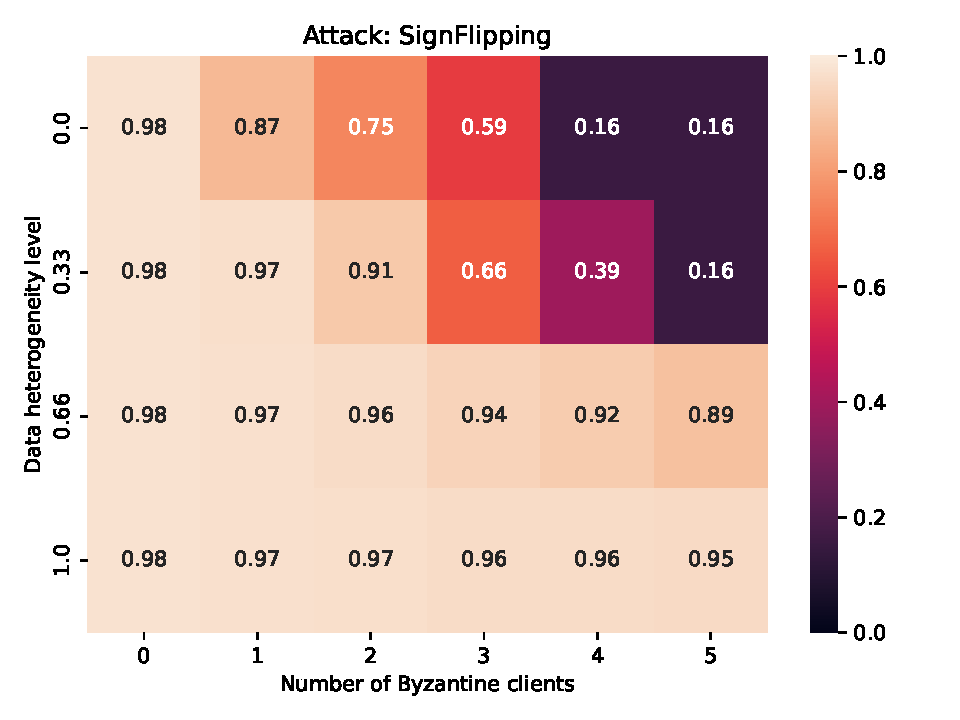
\includegraphics[width=\textwidth]{../activation_clip_plots/cnn_mnist_clip_ramp_1/test_SignFlipping_mnist_cnn_mnist_clip_ramp_1_gamma_similarity_niid_NNM_ARC_MultiKrum_nb_honest_clients_10_tolerated_f_equal_real.pdf}
        \caption{Ramp $C{=}1$ ($r{=}2$)}
        \label{fig:mk_sf_ramp_1}
    \end{subfigure}
    \caption{Multi-Krum (MK) under Sign Flipping Attack.}
    \label{fig:mk_sf_grid}
\end{figure}
\clearpage
\subsection{MK under IPM}
\begin{figure}[htbp]
    \centering
    \begin{subfigure}[b]{0.32\textwidth}
        \centering
        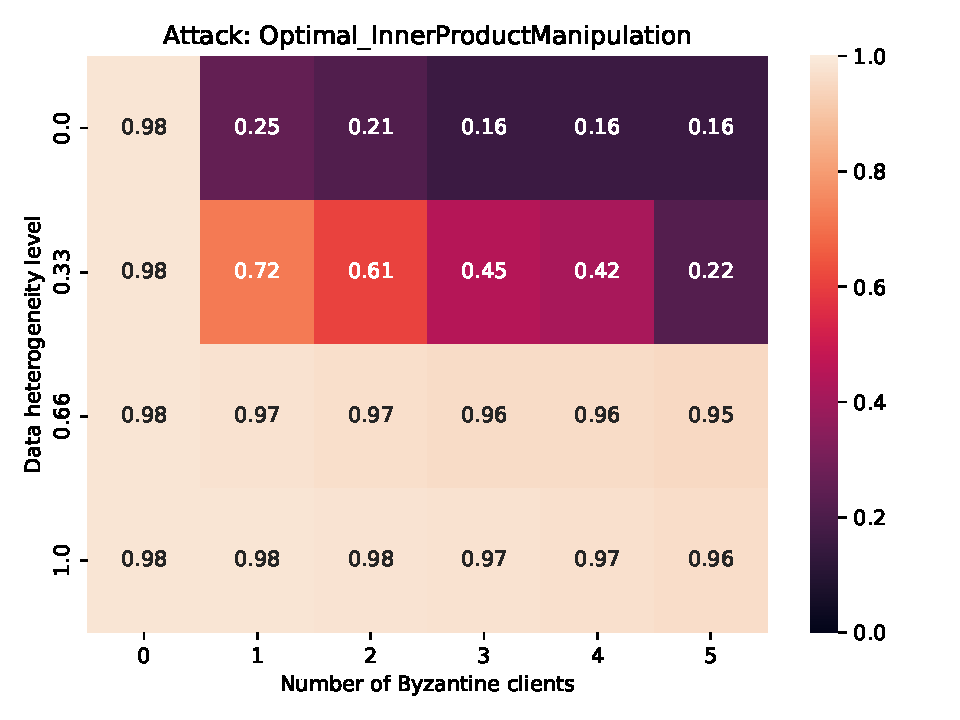
\includegraphics[width=\textwidth]{../plots/mnist_clipping_heatmaps/cnn_mnist/test_Optimal_InnerProductManipulation_mnist_cnn_mnist_gamma_similarity_niid_NNM_ARC_MultiKrum_nb_honest_clients_10_tolerated_f_equal_real.pdf}
        \caption{No Clip (ReLU)}
        \label{fig:mk_ipm_noclip}
    \end{subfigure}
    \hfill
    \begin{subfigure}[b]{0.32\textwidth}
        \centering
        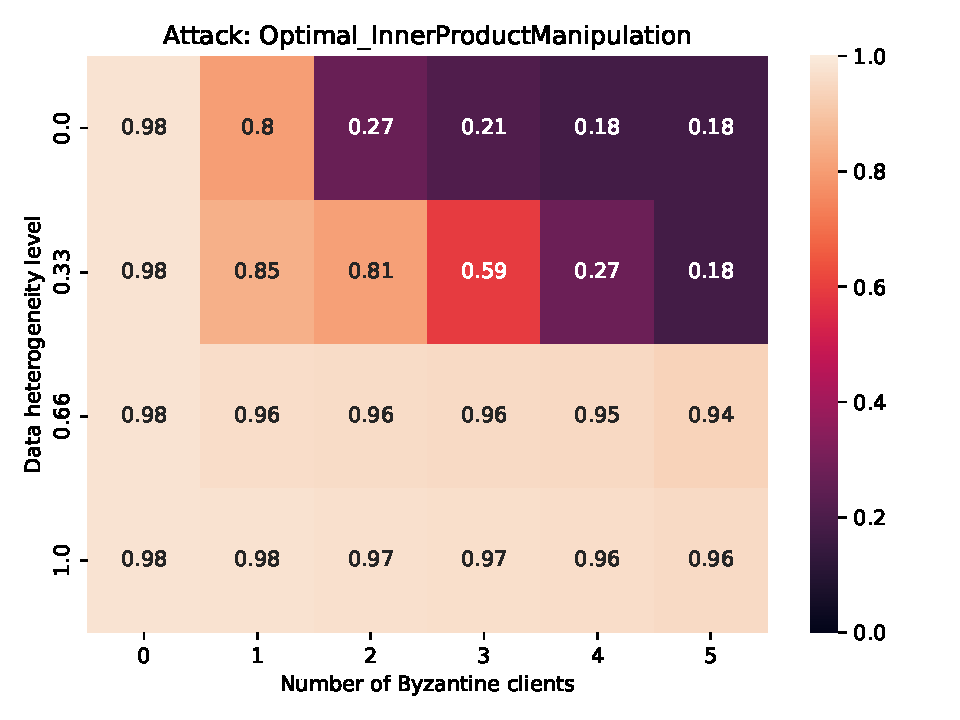
\includegraphics[width=\textwidth]{../plots/cnn_tanh_heatmaps/test_Optimal_InnerProductManipulation_mnist_cnn_mnist_tanh_gamma_similarity_niid_NNM_ARC_MultiKrum_nb_honest_clients_10_tolerated_f_equal_real.pdf}
        \caption{Tanh}
        \label{fig:mk_ipm_tanh}
    \end{subfigure}
    \hfill
    \begin{subfigure}[b]{0.32\textwidth}
        \centering
        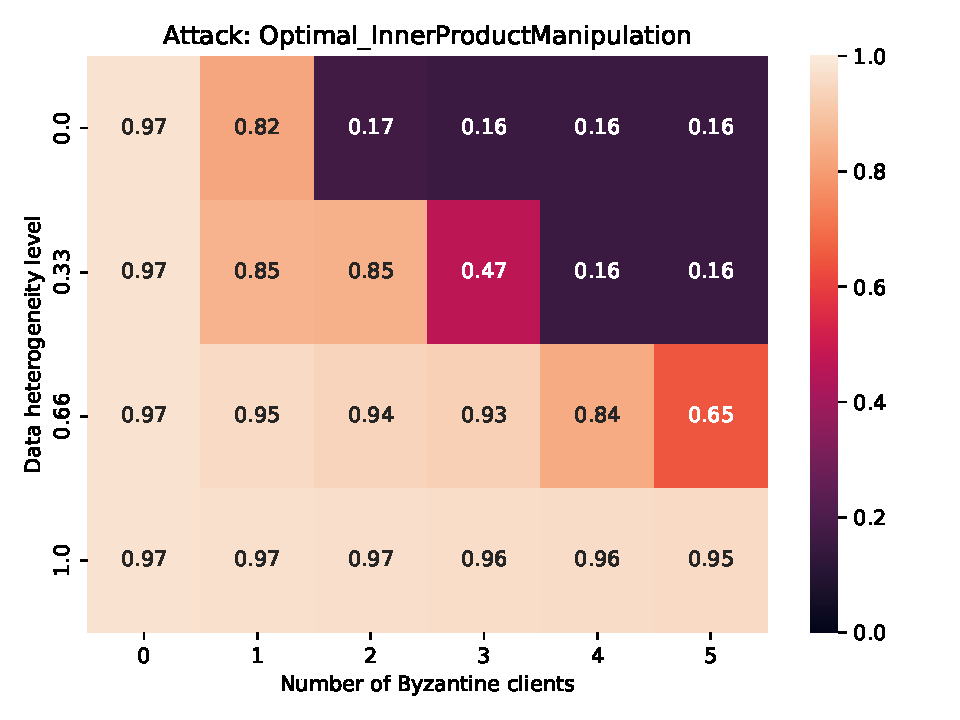
\includegraphics[width=\textwidth]{../plots/mnist_clipping_heatmaps/cnn_mnist_clipping_1/test_Optimal_InnerProductManipulation_mnist_cnn_mnist_clipping_1_gamma_similarity_niid_NNM_ARC_MultiKrum_nb_honest_clients_10_tolerated_f_equal_real.pdf}
        \caption{Hardtanh $C{=}1$}
        \label{fig:mk_ipm_hardtanh_1}
    \end{subfigure}
    \vspace{0.3cm}
    \begin{subfigure}[b]{0.32\textwidth}
        \centering
        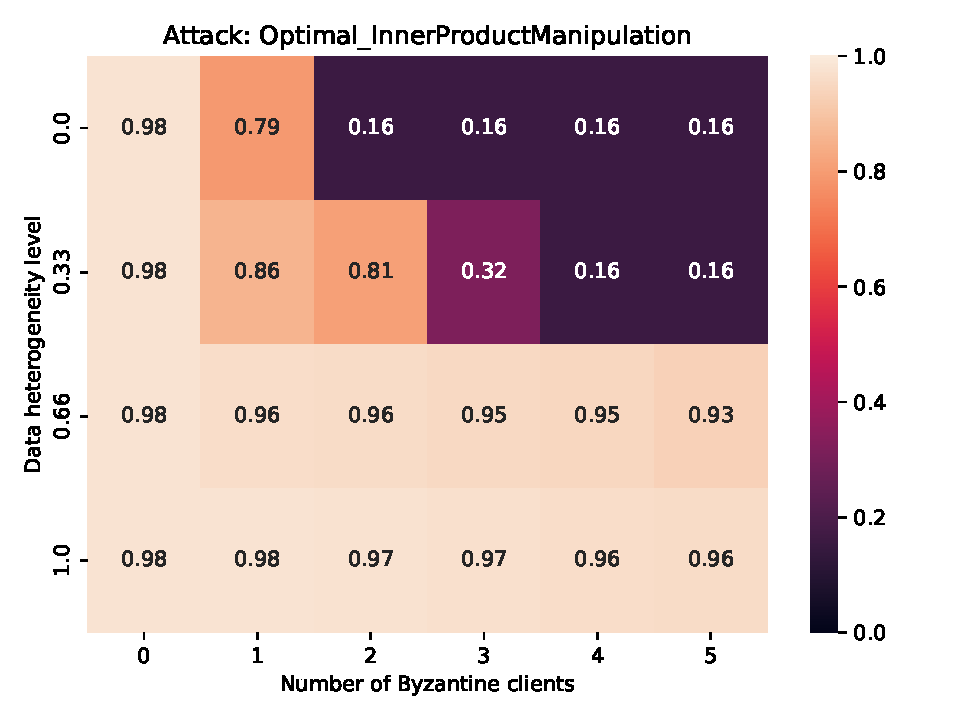
\includegraphics[width=\textwidth]{../plots/mnist_clipping_heatmaps/cnn_mnist_clipping_2/test_Optimal_InnerProductManipulation_mnist_cnn_mnist_clipping_2_gamma_similarity_niid_NNM_ARC_MultiKrum_nb_honest_clients_10_tolerated_f_equal_real.pdf}
        \caption{Hardtanh $C{=}2$}
        \label{fig:mk_ipm_hardtanh_2}
    \end{subfigure}
    \hfill
    \begin{subfigure}[b]{0.32\textwidth}
        \centering
        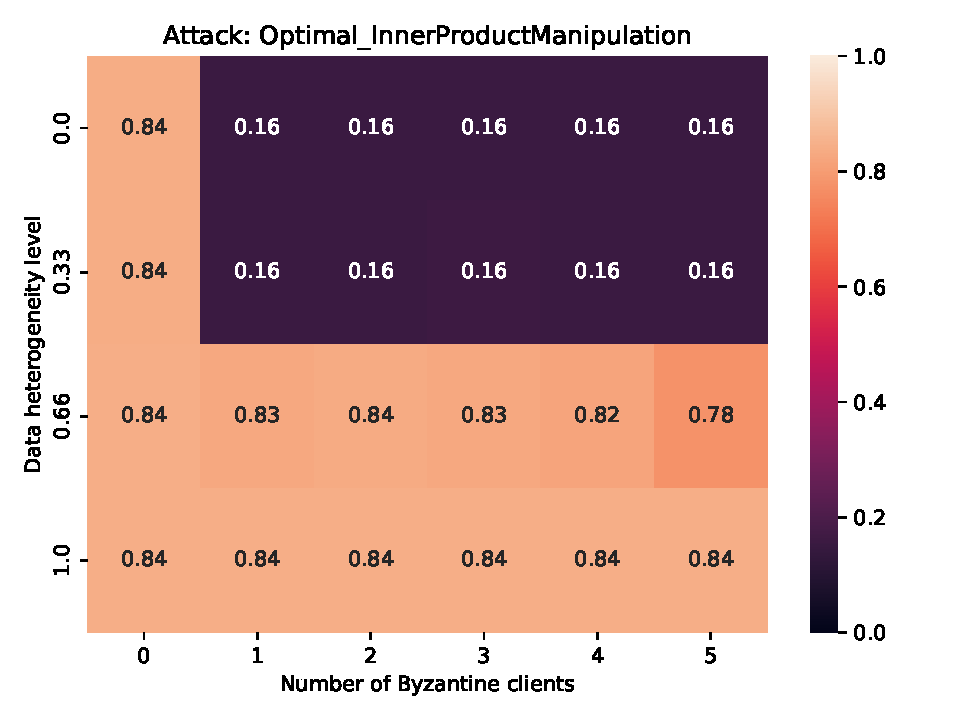
\includegraphics[width=\textwidth]{../activation_clip_plots/cnn_mnist_clip_ste_1/test_Optimal_InnerProductManipulation_mnist_cnn_mnist_clip_ste_1_gamma_similarity_niid_NNM_ARC_MultiKrum_nb_honest_clients_10_tolerated_f_equal_real.pdf}
        \caption{STE $C{=}1$}
        \label{fig:mk_ipm_ste_1}
    \end{subfigure}
    \hfill
    \begin{subfigure}[b]{0.32\textwidth}
        \centering
        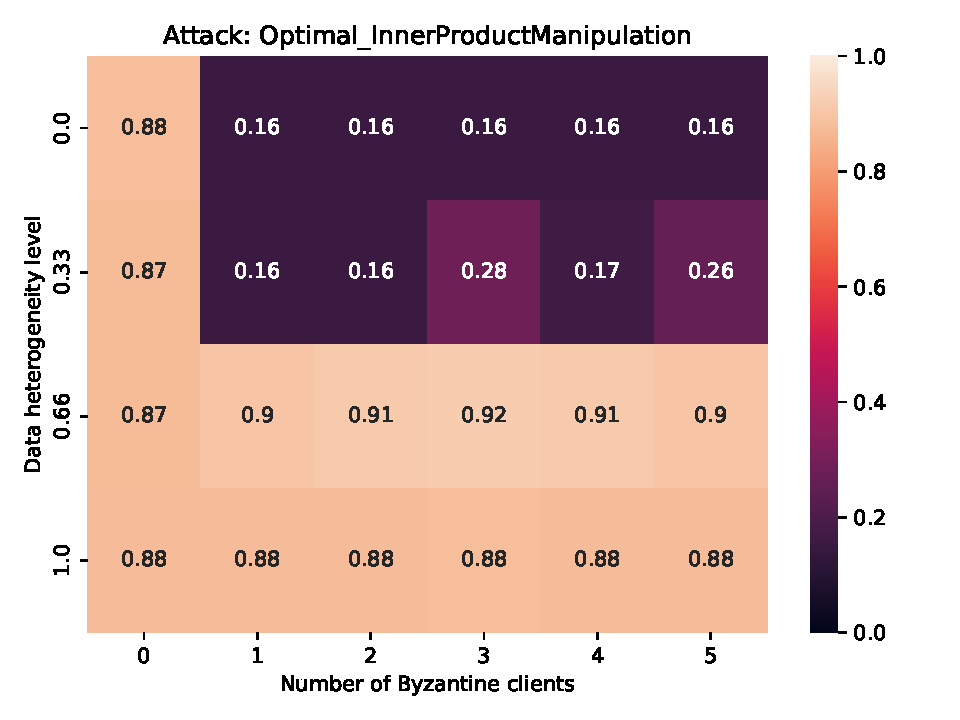
\includegraphics[width=\textwidth]{../activation_clip_plots/cnn_mnist_clip_ste_2/test_Optimal_InnerProductManipulation_mnist_cnn_mnist_clip_ste_2_gamma_similarity_niid_NNM_ARC_MultiKrum_nb_honest_clients_10_tolerated_f_equal_real.pdf}
        \caption{STE $C{=}2$}
        \label{fig:mk_ipm_ste_2}
    \end{subfigure}
    \vspace{0.3cm}
    \begin{subfigure}[b]{0.32\textwidth}
        \centering
        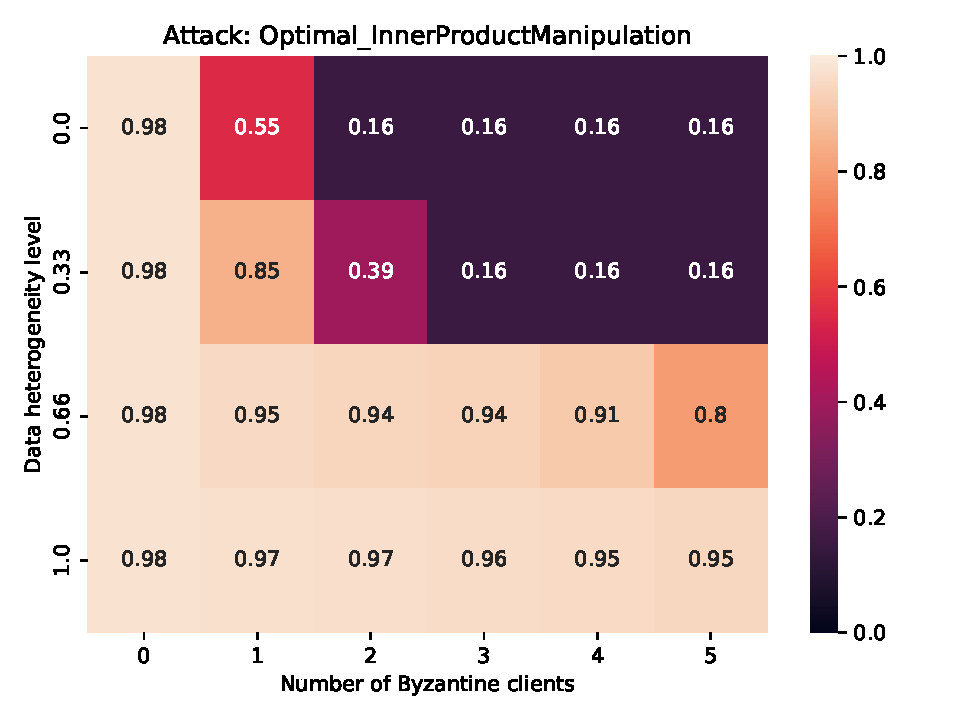
\includegraphics[width=\textwidth]{../activation_clip_plots/cnn_mnist_clip_ramp_1/test_Optimal_InnerProductManipulation_mnist_cnn_mnist_clip_ramp_1_gamma_similarity_niid_NNM_ARC_MultiKrum_nb_honest_clients_10_tolerated_f_equal_real.pdf}
        \caption{Ramp $C{=}1$ ($r{=}2$)}
        \label{fig:mk_ipm_ramp_1}
    \end{subfigure}
    \caption{Multi-Krum (MK) under Optimal IPM Attack.}
    \label{fig:mk_ipm_grid}
\end{figure}
\clearpage
\section{Trimmed Mean (TM)}
\subsection{TM under Worst-Case across all Attacks}
\begin{figure}[htbp]
    \centering
    \begin{subfigure}[b]{0.32\textwidth}
        \centering
        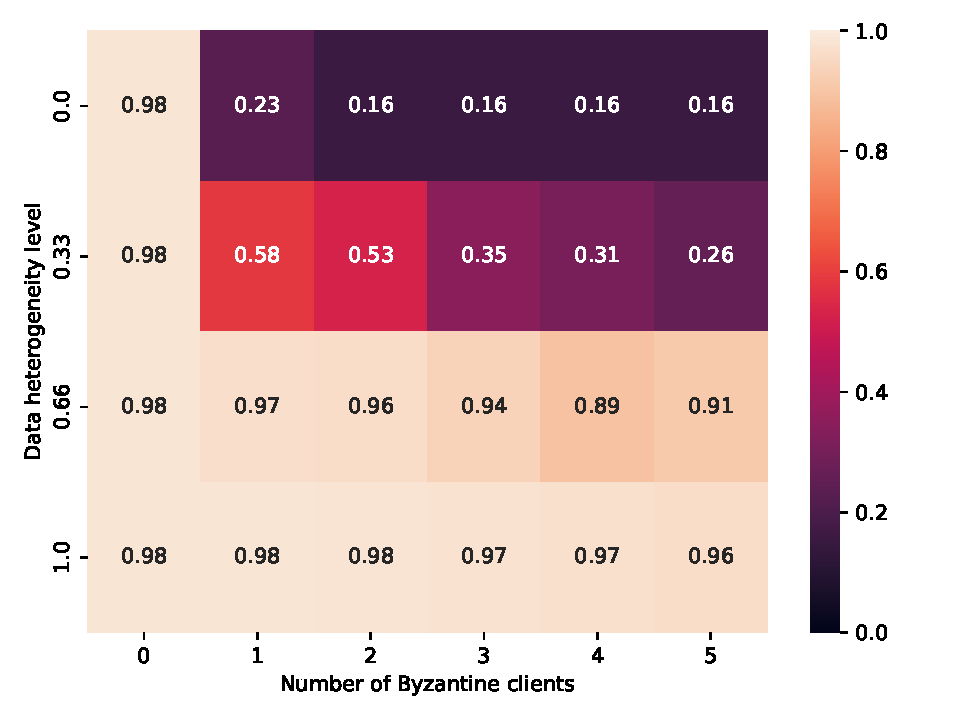
\includegraphics[width=\textwidth]{../plots/mnist_clipping_heatmaps/cnn_mnist/test_mnist_cnn_mnist_gamma_similarity_niid_NNM_ARC_TrMean_nb_honest_clients_10_tolerated_f_equal_real.pdf}
        \caption{No Clip (ReLU)}
        \label{fig:tm_worst_case_noclip}
    \end{subfigure}
    \hfill
    \begin{subfigure}[b]{0.32\textwidth}
        \centering
        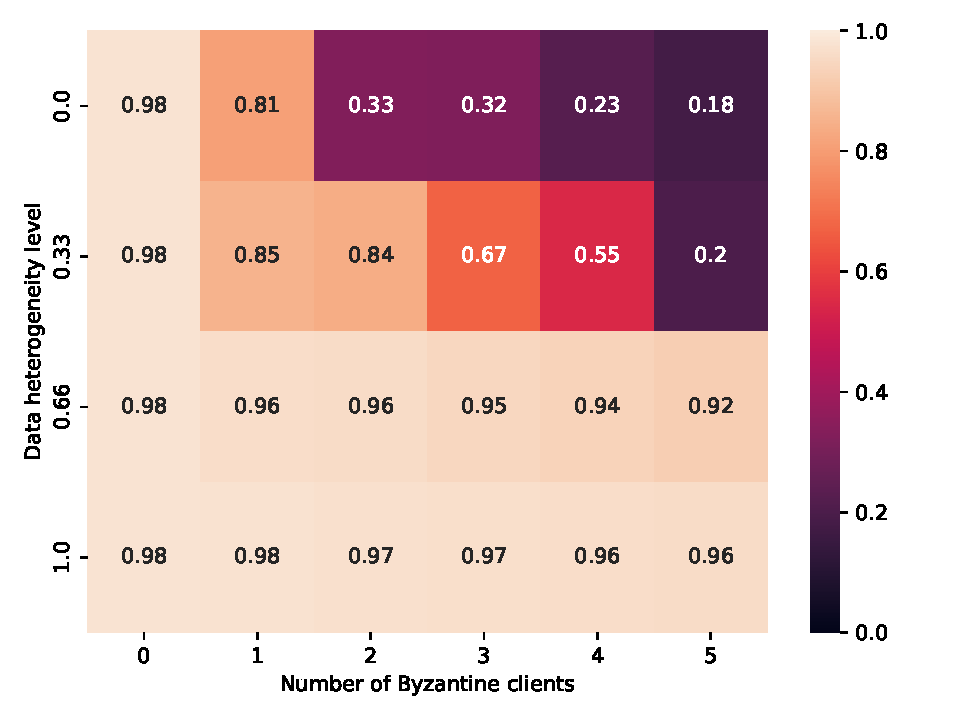
\includegraphics[width=\textwidth]{../plots/cnn_tanh_heatmaps/test_mnist_cnn_mnist_tanh_gamma_similarity_niid_NNM_ARC_TrMean_nb_honest_clients_10_tolerated_f_equal_real.pdf}
        \caption{Tanh}
        \label{fig:tm_worst_case_tanh}
    \end{subfigure}
    \hfill
    \begin{subfigure}[b]{0.32\textwidth}
        \centering
        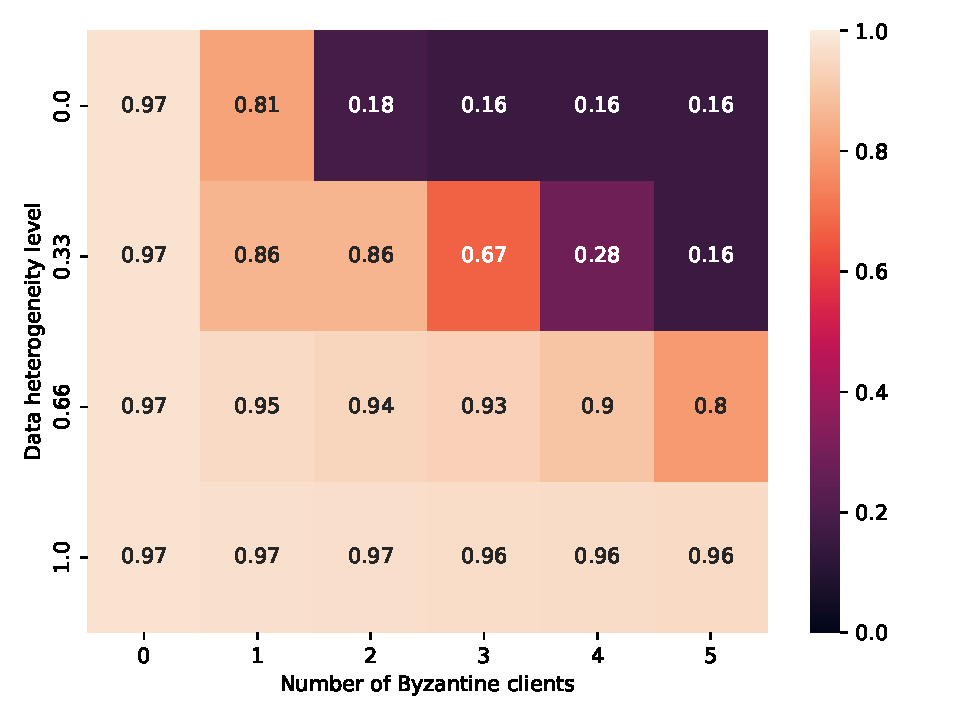
\includegraphics[width=\textwidth]{../plots/mnist_clipping_heatmaps/cnn_mnist_clipping_1/test_mnist_cnn_mnist_clipping_1_gamma_similarity_niid_NNM_ARC_TrMean_nb_honest_clients_10_tolerated_f_equal_real.pdf}
        \caption{Hardtanh $C{=}1$}
        \label{fig:tm_worst_case_hardtanh_1}
    \end{subfigure}
    \vspace{0.3cm}
    \begin{subfigure}[b]{0.32\textwidth}
        \centering
        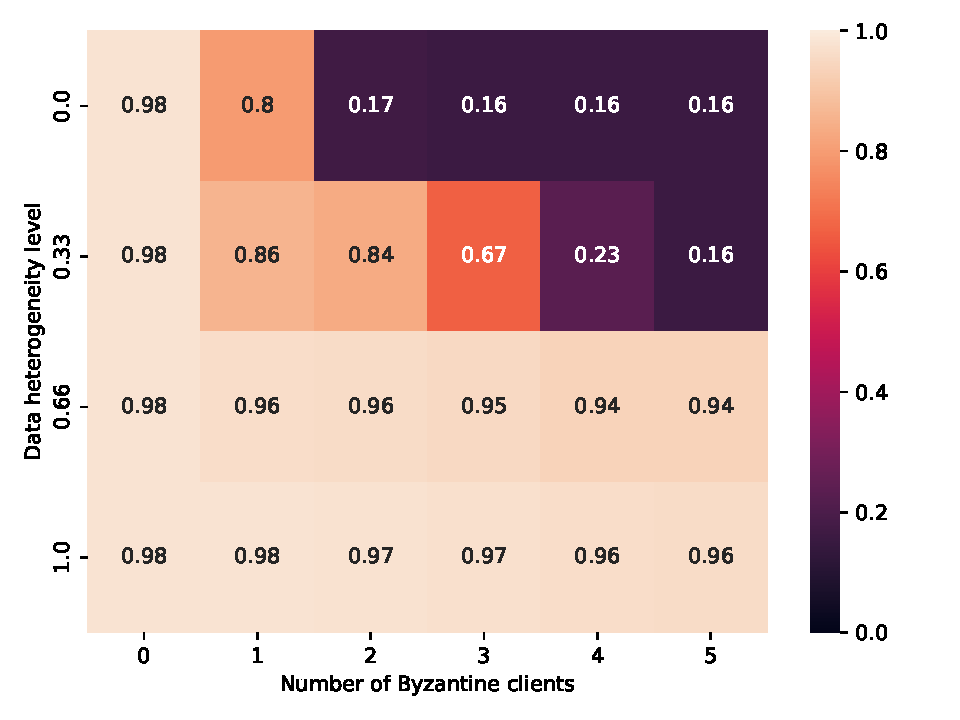
\includegraphics[width=\textwidth]{../plots/mnist_clipping_heatmaps/cnn_mnist_clipping_2/test_mnist_cnn_mnist_clipping_2_gamma_similarity_niid_NNM_ARC_TrMean_nb_honest_clients_10_tolerated_f_equal_real.pdf}
        \caption{Hardtanh $C{=}2$}
        \label{fig:tm_worst_case_hardtanh_2}
    \end{subfigure}
    \hfill
    \begin{subfigure}[b]{0.32\textwidth}
        \centering
        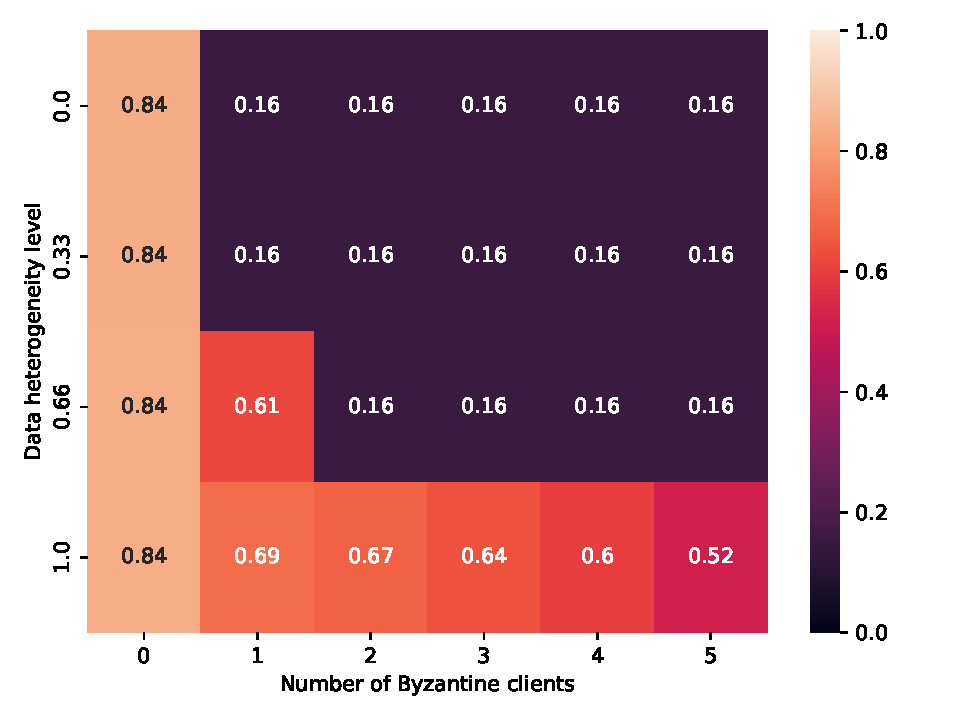
\includegraphics[width=\textwidth]{../activation_clip_plots/cnn_mnist_clip_ste_1/test_mnist_cnn_mnist_clip_ste_1_gamma_similarity_niid_NNM_ARC_TrMean_nb_honest_clients_10_tolerated_f_equal_real.pdf}
        \caption{STE $C{=}1$}
        \label{fig:tm_worst_case_ste_1}
    \end{subfigure}
    \hfill
    \begin{subfigure}[b]{0.32\textwidth}
        \centering
        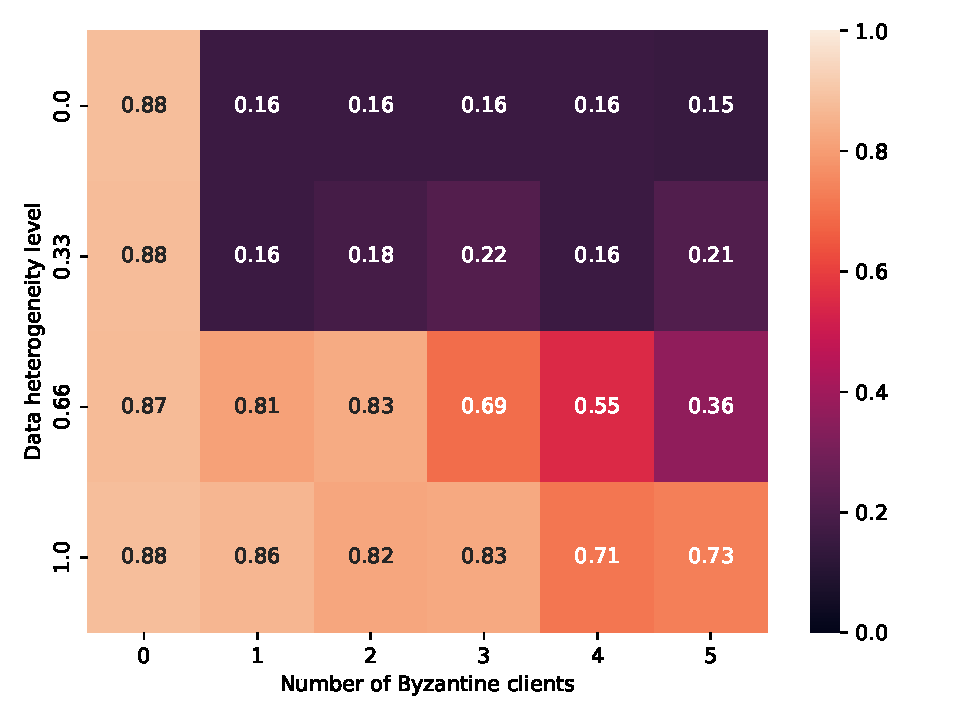
\includegraphics[width=\textwidth]{../activation_clip_plots/cnn_mnist_clip_ste_2/test_mnist_cnn_mnist_clip_ste_2_gamma_similarity_niid_NNM_ARC_TrMean_nb_honest_clients_10_tolerated_f_equal_real.pdf}
        \caption{STE $C{=}2$}
        \label{fig:tm_worst_case_ste_2}
    \end{subfigure}
    \vspace{0.3cm}
    \begin{subfigure}[b]{0.32\textwidth}
        \centering
        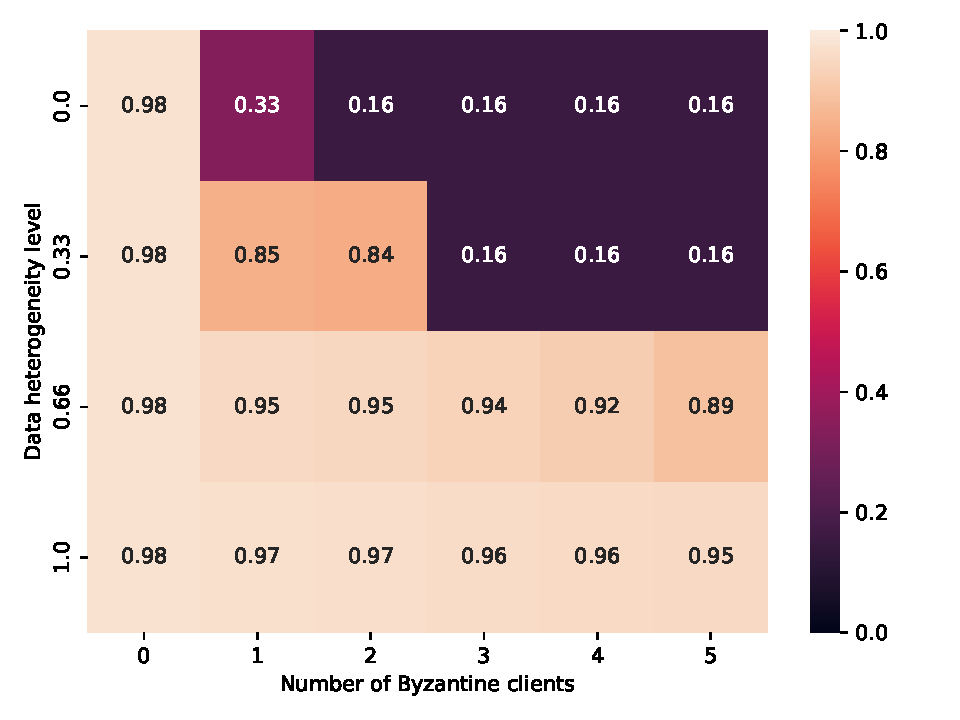
\includegraphics[width=\textwidth]{../activation_clip_plots/cnn_mnist_clip_ramp_1/test_mnist_cnn_mnist_clip_ramp_1_gamma_similarity_niid_NNM_ARC_TrMean_nb_honest_clients_10_tolerated_f_equal_real.pdf}
        \caption{Ramp $C{=}1$ ($r{=}2$)}
        \label{fig:tm_worst_case_ramp_1}
    \end{subfigure}
    \caption{Trimmed Mean (TM) under Worst-Case across all Attacks.}
    \label{fig:tm_worst_case_grid}
\end{figure}
\clearpage
\subsection{TM under ALIE}
\begin{figure}[htbp]
    \centering
    \begin{subfigure}[b]{0.32\textwidth}
        \centering
        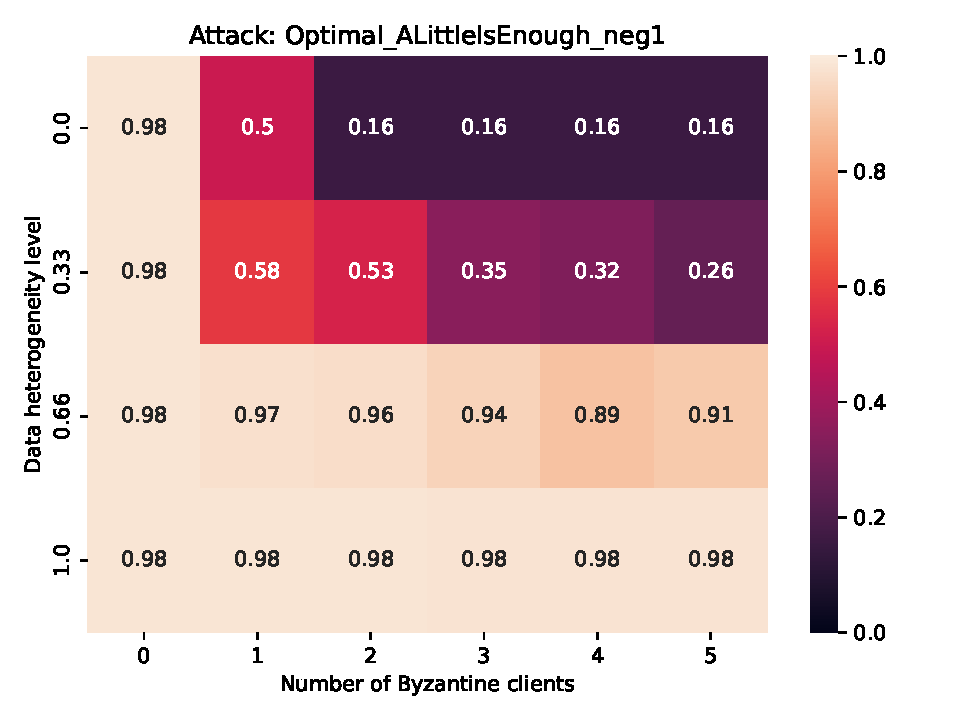
\includegraphics[width=\textwidth]{../plots/mnist_clipping_heatmaps/cnn_mnist/test_Optimal_ALittleIsEnough_neg1_mnist_cnn_mnist_gamma_similarity_niid_NNM_ARC_TrMean_nb_honest_clients_10_tolerated_f_equal_real.pdf}
        \caption{No Clip (ReLU)}
        \label{fig:tm_alie_noclip}
    \end{subfigure}
    \hfill
    \begin{subfigure}[b]{0.32\textwidth}
        \centering
        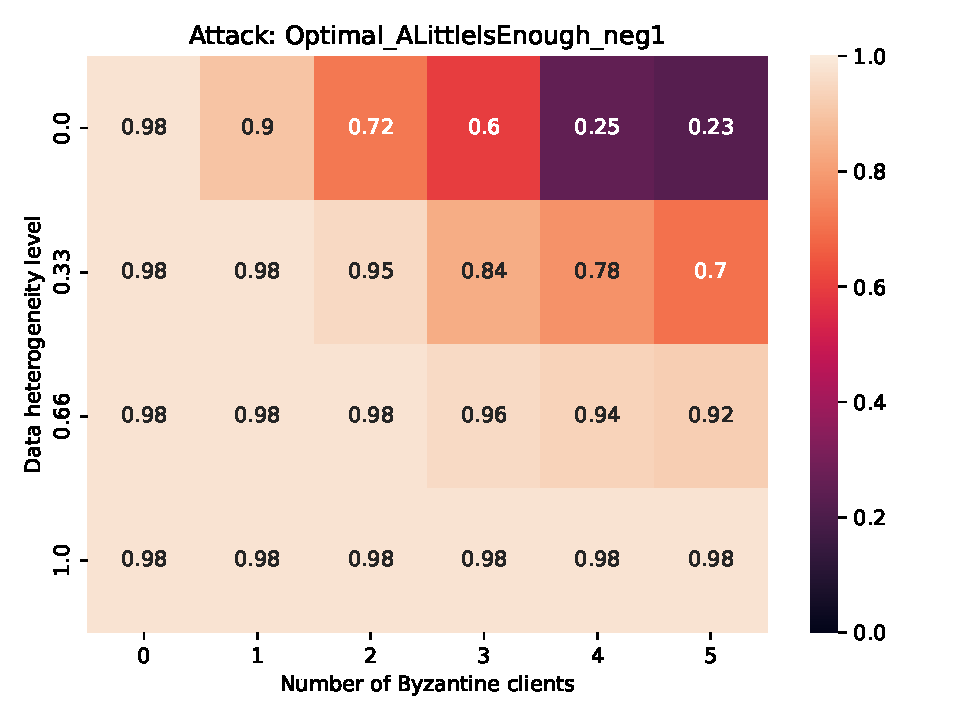
\includegraphics[width=\textwidth]{../plots/cnn_tanh_heatmaps/test_Optimal_ALittleIsEnough_neg1_mnist_cnn_mnist_tanh_gamma_similarity_niid_NNM_ARC_TrMean_nb_honest_clients_10_tolerated_f_equal_real.pdf}
        \caption{Tanh}
        \label{fig:tm_alie_tanh}
    \end{subfigure}
    \hfill
    \begin{subfigure}[b]{0.32\textwidth}
        \centering
        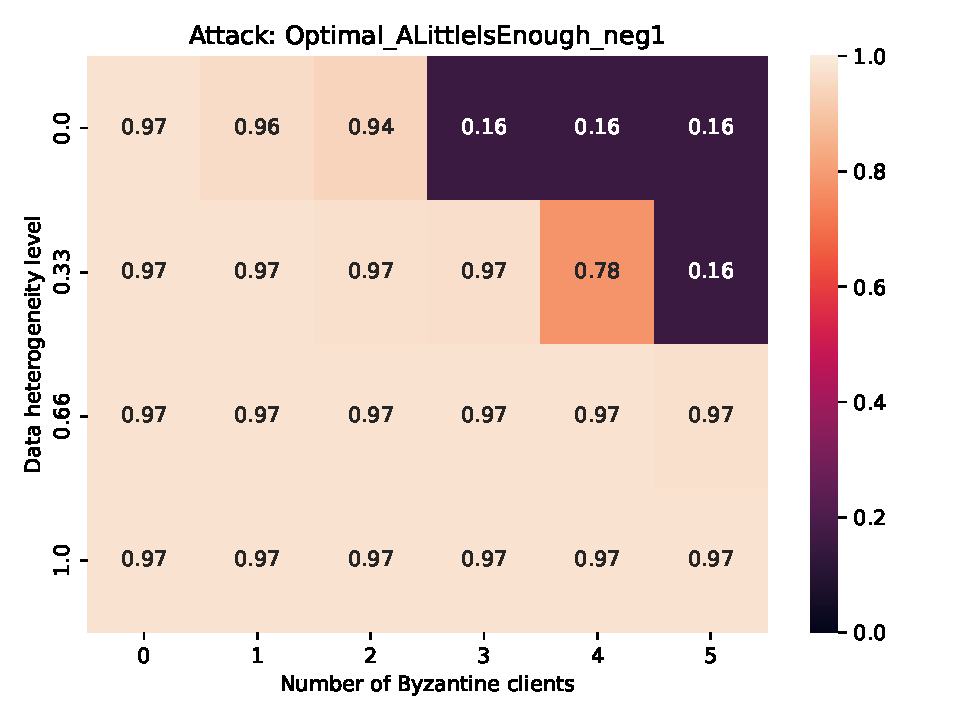
\includegraphics[width=\textwidth]{../plots/mnist_clipping_heatmaps/cnn_mnist_clipping_1/test_Optimal_ALittleIsEnough_neg1_mnist_cnn_mnist_clipping_1_gamma_similarity_niid_NNM_ARC_TrMean_nb_honest_clients_10_tolerated_f_equal_real.pdf}
        \caption{Hardtanh $C{=}1$}
        \label{fig:tm_alie_hardtanh_1}
    \end{subfigure}
    \vspace{0.3cm}
    \begin{subfigure}[b]{0.32\textwidth}
        \centering
        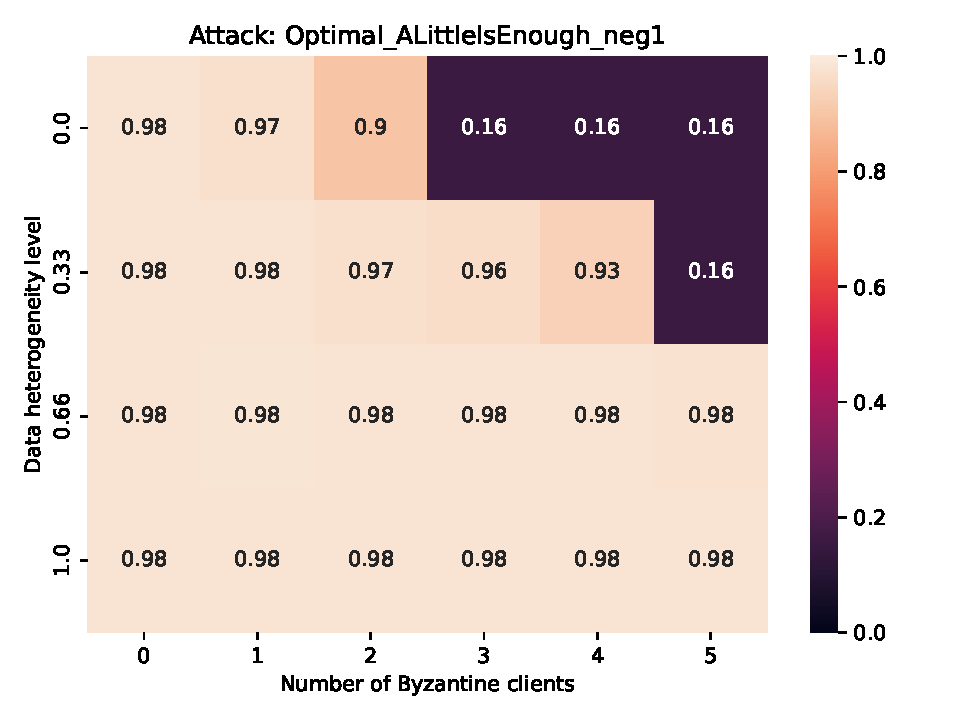
\includegraphics[width=\textwidth]{../plots/mnist_clipping_heatmaps/cnn_mnist_clipping_2/test_Optimal_ALittleIsEnough_neg1_mnist_cnn_mnist_clipping_2_gamma_similarity_niid_NNM_ARC_TrMean_nb_honest_clients_10_tolerated_f_equal_real.pdf}
        \caption{Hardtanh $C{=}2$}
        \label{fig:tm_alie_hardtanh_2}
    \end{subfigure}
    \hfill
    \begin{subfigure}[b]{0.32\textwidth}
        \centering
        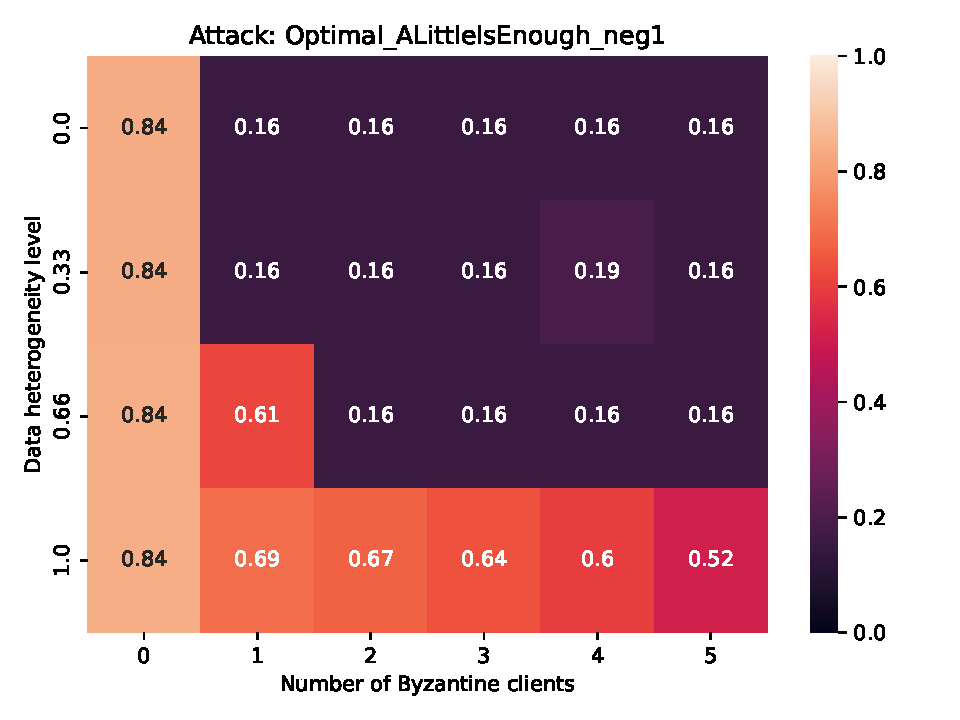
\includegraphics[width=\textwidth]{../activation_clip_plots/cnn_mnist_clip_ste_1/test_Optimal_ALittleIsEnough_neg1_mnist_cnn_mnist_clip_ste_1_gamma_similarity_niid_NNM_ARC_TrMean_nb_honest_clients_10_tolerated_f_equal_real.pdf}
        \caption{STE $C{=}1$}
        \label{fig:tm_alie_ste_1}
    \end{subfigure}
    \hfill
    \begin{subfigure}[b]{0.32\textwidth}
        \centering
        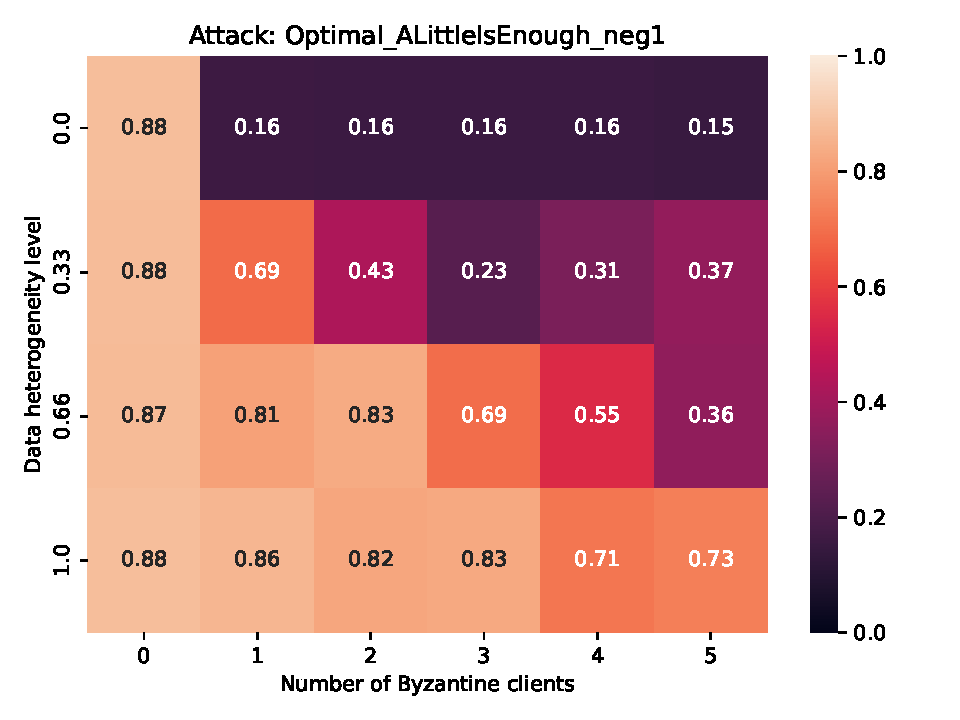
\includegraphics[width=\textwidth]{../activation_clip_plots/cnn_mnist_clip_ste_2/test_Optimal_ALittleIsEnough_neg1_mnist_cnn_mnist_clip_ste_2_gamma_similarity_niid_NNM_ARC_TrMean_nb_honest_clients_10_tolerated_f_equal_real.pdf}
        \caption{STE $C{=}2$}
        \label{fig:tm_alie_ste_2}
    \end{subfigure}
    \vspace{0.3cm}
    \begin{subfigure}[b]{0.32\textwidth}
        \centering
        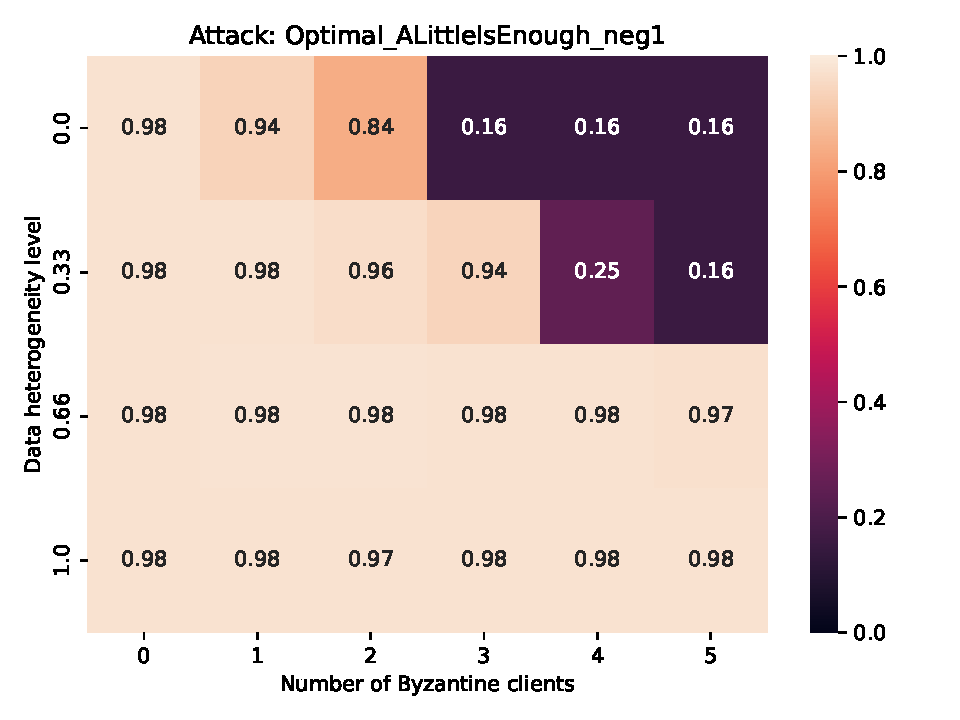
\includegraphics[width=\textwidth]{../activation_clip_plots/cnn_mnist_clip_ramp_1/test_Optimal_ALittleIsEnough_neg1_mnist_cnn_mnist_clip_ramp_1_gamma_similarity_niid_NNM_ARC_TrMean_nb_honest_clients_10_tolerated_f_equal_real.pdf}
        \caption{Ramp $C{=}1$ ($r{=}2$)}
        \label{fig:tm_alie_ramp_1}
    \end{subfigure}
    \caption{Trimmed Mean (TM) under Optimal ALIE Attack.}
    \label{fig:tm_alie_grid}
\end{figure}
\clearpage
\subsection{TM under SF}
\begin{figure}[htbp]
    \centering
    \begin{subfigure}[b]{0.32\textwidth}
        \centering
        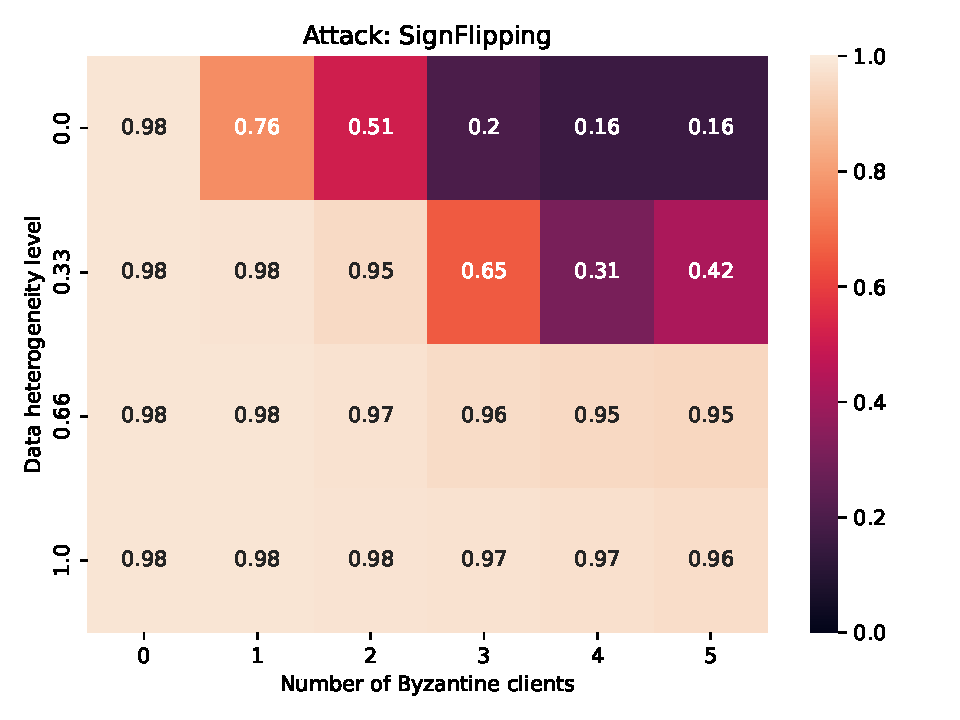
\includegraphics[width=\textwidth]{../plots/mnist_clipping_heatmaps/cnn_mnist/test_SignFlipping_mnist_cnn_mnist_gamma_similarity_niid_NNM_ARC_TrMean_nb_honest_clients_10_tolerated_f_equal_real.pdf}
        \caption{No Clip (ReLU)}
        \label{fig:tm_sf_noclip}
    \end{subfigure}
    \hfill
    \begin{subfigure}[b]{0.32\textwidth}
        \centering
        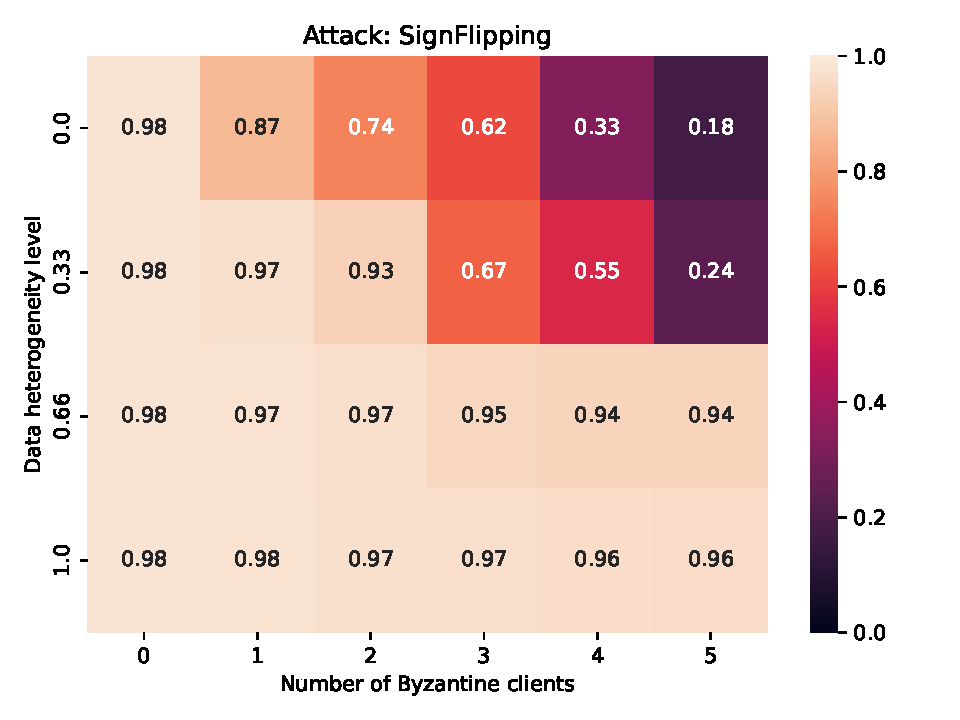
\includegraphics[width=\textwidth]{../plots/cnn_tanh_heatmaps/test_SignFlipping_mnist_cnn_mnist_tanh_gamma_similarity_niid_NNM_ARC_TrMean_nb_honest_clients_10_tolerated_f_equal_real.pdf}
        \caption{Tanh}
        \label{fig:tm_sf_tanh}
    \end{subfigure}
    \hfill
    \begin{subfigure}[b]{0.32\textwidth}
        \centering
        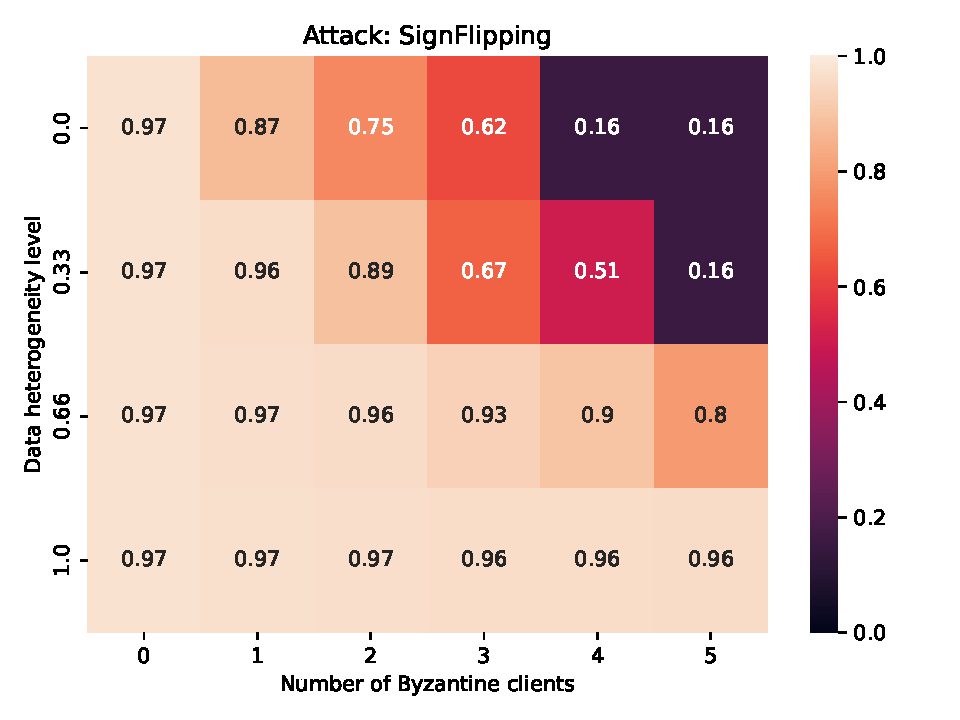
\includegraphics[width=\textwidth]{../plots/mnist_clipping_heatmaps/cnn_mnist_clipping_1/test_SignFlipping_mnist_cnn_mnist_clipping_1_gamma_similarity_niid_NNM_ARC_TrMean_nb_honest_clients_10_tolerated_f_equal_real.pdf}
        \caption{Hardtanh $C{=}1$}
        \label{fig:tm_sf_hardtanh_1}
    \end{subfigure}
    \vspace{0.3cm}
    \begin{subfigure}[b]{0.32\textwidth}
        \centering
        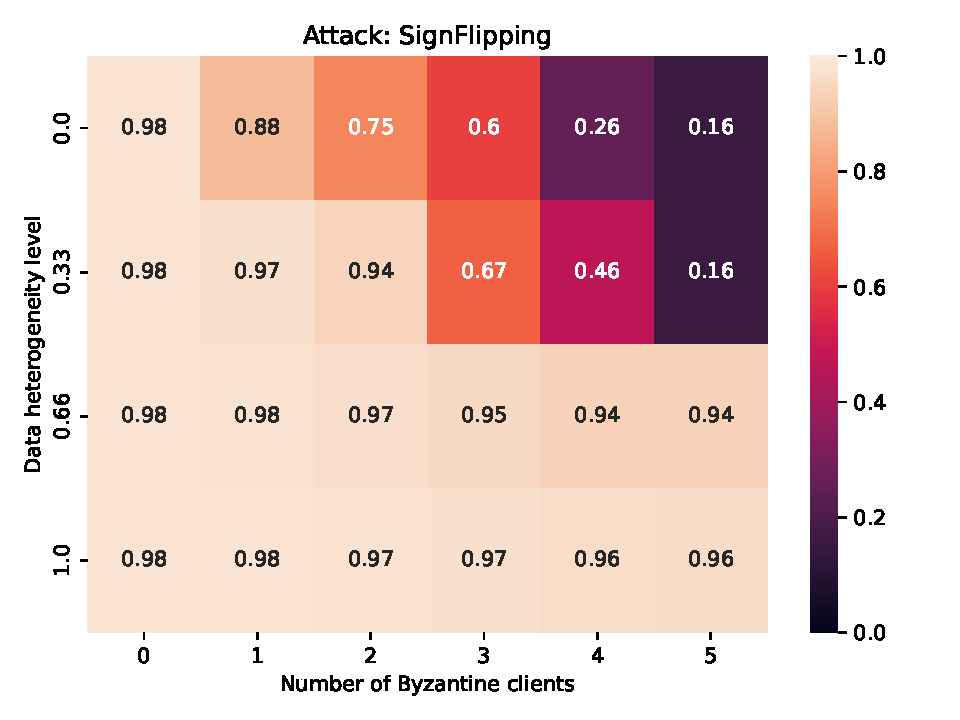
\includegraphics[width=\textwidth]{../plots/mnist_clipping_heatmaps/cnn_mnist_clipping_2/test_SignFlipping_mnist_cnn_mnist_clipping_2_gamma_similarity_niid_NNM_ARC_TrMean_nb_honest_clients_10_tolerated_f_equal_real.pdf}
        \caption{Hardtanh $C{=}2$}
        \label{fig:tm_sf_hardtanh_2}
    \end{subfigure}
    \hfill
    \begin{subfigure}[b]{0.32\textwidth}
        \centering
        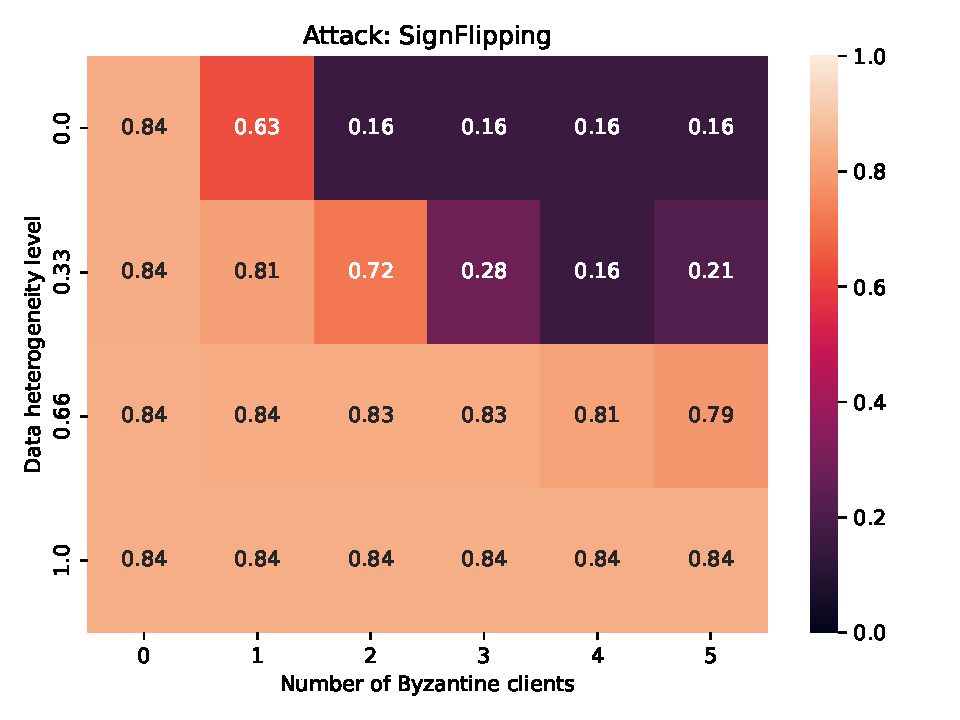
\includegraphics[width=\textwidth]{../activation_clip_plots/cnn_mnist_clip_ste_1/test_SignFlipping_mnist_cnn_mnist_clip_ste_1_gamma_similarity_niid_NNM_ARC_TrMean_nb_honest_clients_10_tolerated_f_equal_real.pdf}
        \caption{STE $C{=}1$}
        \label{fig:tm_sf_ste_1}
    \end{subfigure}
    \hfill
    \begin{subfigure}[b]{0.32\textwidth}
        \centering
        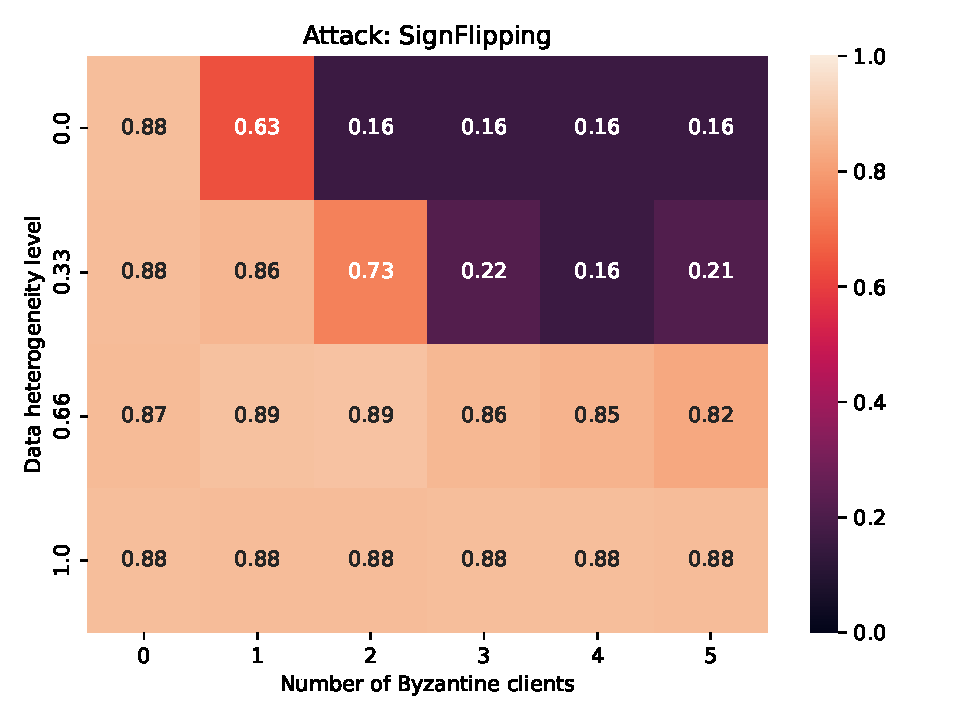
\includegraphics[width=\textwidth]{../activation_clip_plots/cnn_mnist_clip_ste_2/test_SignFlipping_mnist_cnn_mnist_clip_ste_2_gamma_similarity_niid_NNM_ARC_TrMean_nb_honest_clients_10_tolerated_f_equal_real.pdf}
        \caption{STE $C{=}2$}
        \label{fig:tm_sf_ste_2}
    \end{subfigure}
    \vspace{0.3cm}
    \begin{subfigure}[b]{0.32\textwidth}
        \centering
        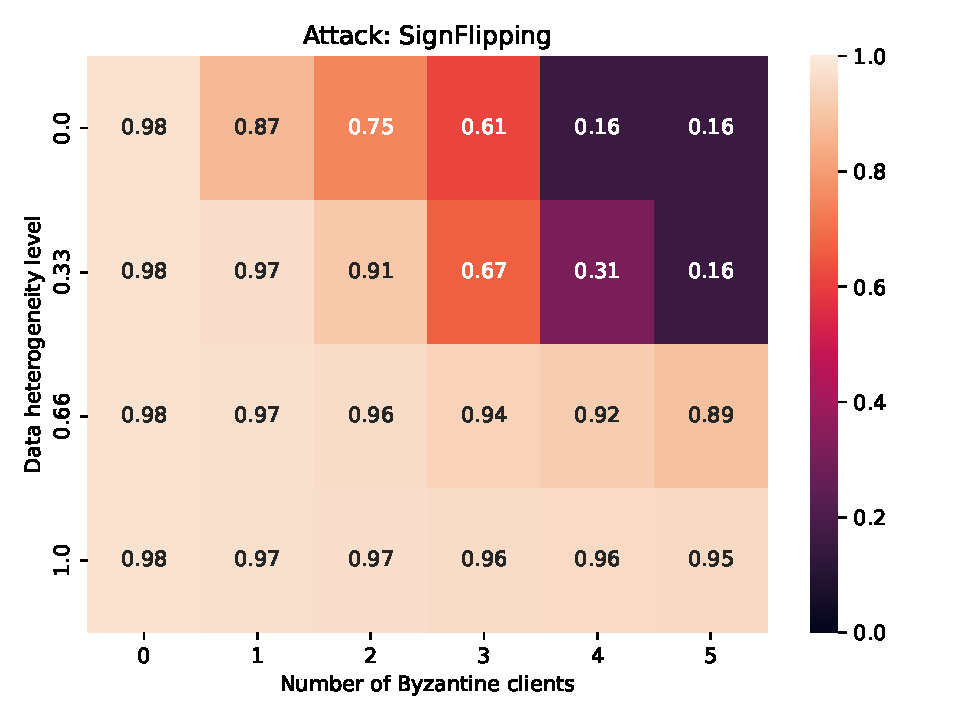
\includegraphics[width=\textwidth]{../activation_clip_plots/cnn_mnist_clip_ramp_1/test_SignFlipping_mnist_cnn_mnist_clip_ramp_1_gamma_similarity_niid_NNM_ARC_TrMean_nb_honest_clients_10_tolerated_f_equal_real.pdf}
        \caption{Ramp $C{=}1$ ($r{=}2$)}
        \label{fig:tm_sf_ramp_1}
    \end{subfigure}
    \caption{Trimmed Mean (TM) under Sign Flipping Attack.}
    \label{fig:tm_sf_grid}
\end{figure}
\clearpage
\subsection{TM under IPM}
\begin{figure}[htbp]
    \centering
    \begin{subfigure}[b]{0.32\textwidth}
        \centering
        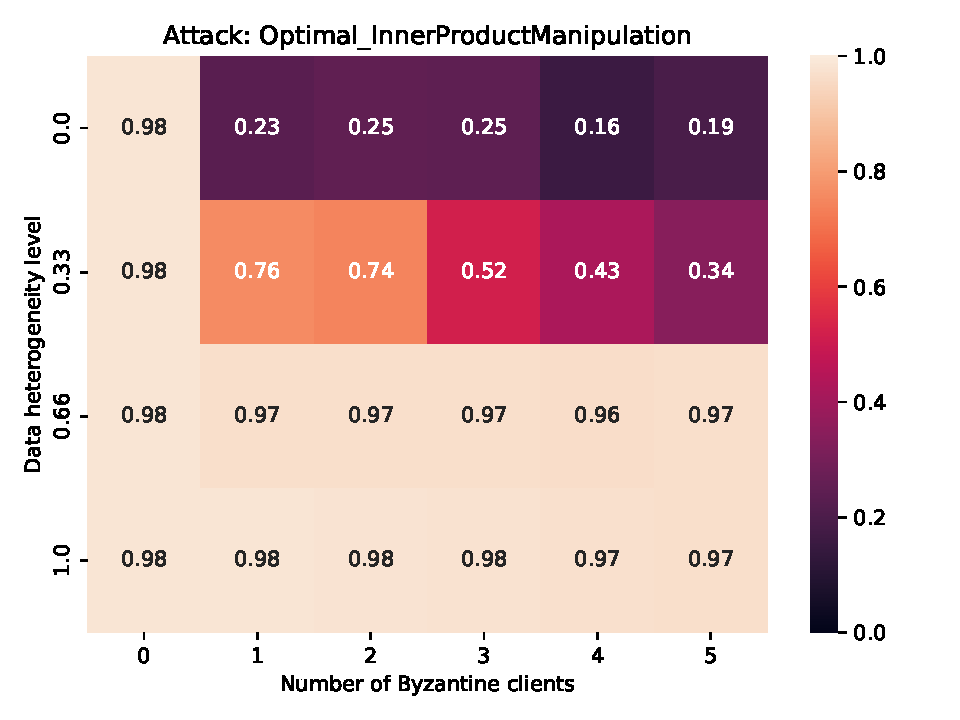
\includegraphics[width=\textwidth]{../plots/mnist_clipping_heatmaps/cnn_mnist/test_Optimal_InnerProductManipulation_mnist_cnn_mnist_gamma_similarity_niid_NNM_ARC_TrMean_nb_honest_clients_10_tolerated_f_equal_real.pdf}
        \caption{No Clip (ReLU)}
        \label{fig:tm_ipm_noclip}
    \end{subfigure}
    \hfill
    \begin{subfigure}[b]{0.32\textwidth}
        \centering
        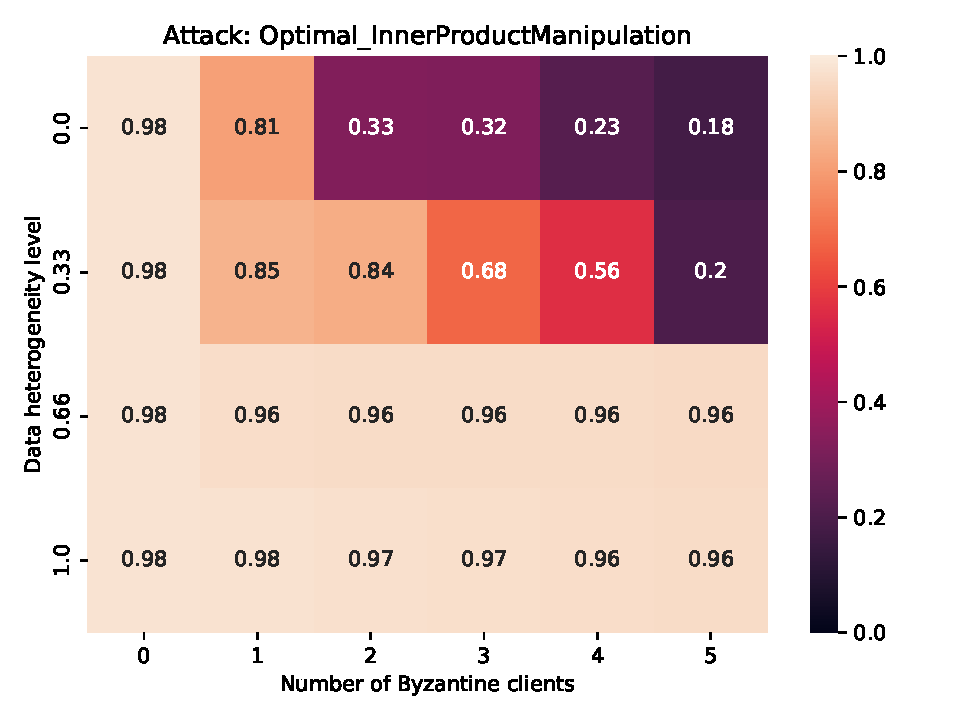
\includegraphics[width=\textwidth]{../plots/cnn_tanh_heatmaps/test_Optimal_InnerProductManipulation_mnist_cnn_mnist_tanh_gamma_similarity_niid_NNM_ARC_TrMean_nb_honest_clients_10_tolerated_f_equal_real.pdf}
        \caption{Tanh}
        \label{fig:tm_ipm_tanh}
    \end{subfigure}
    \hfill
    \begin{subfigure}[b]{0.32\textwidth}
        \centering
        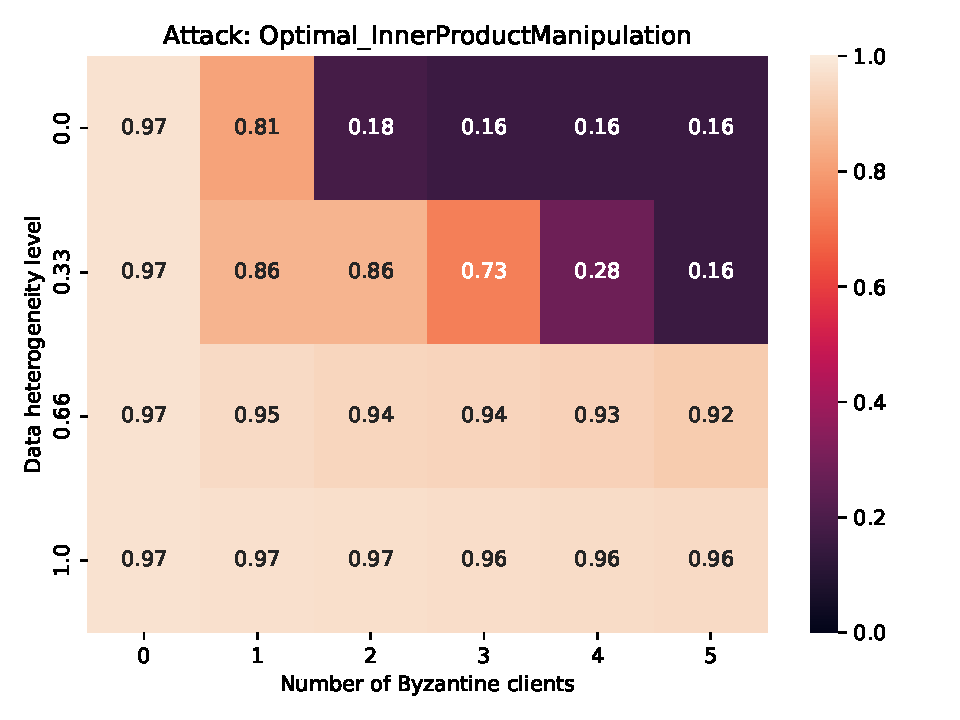
\includegraphics[width=\textwidth]{../plots/mnist_clipping_heatmaps/cnn_mnist_clipping_1/test_Optimal_InnerProductManipulation_mnist_cnn_mnist_clipping_1_gamma_similarity_niid_NNM_ARC_TrMean_nb_honest_clients_10_tolerated_f_equal_real.pdf}
        \caption{Hardtanh $C{=}1$}
        \label{fig:tm_ipm_hardtanh_1}
    \end{subfigure}
    \vspace{0.3cm}
    \begin{subfigure}[b]{0.32\textwidth}
        \centering
        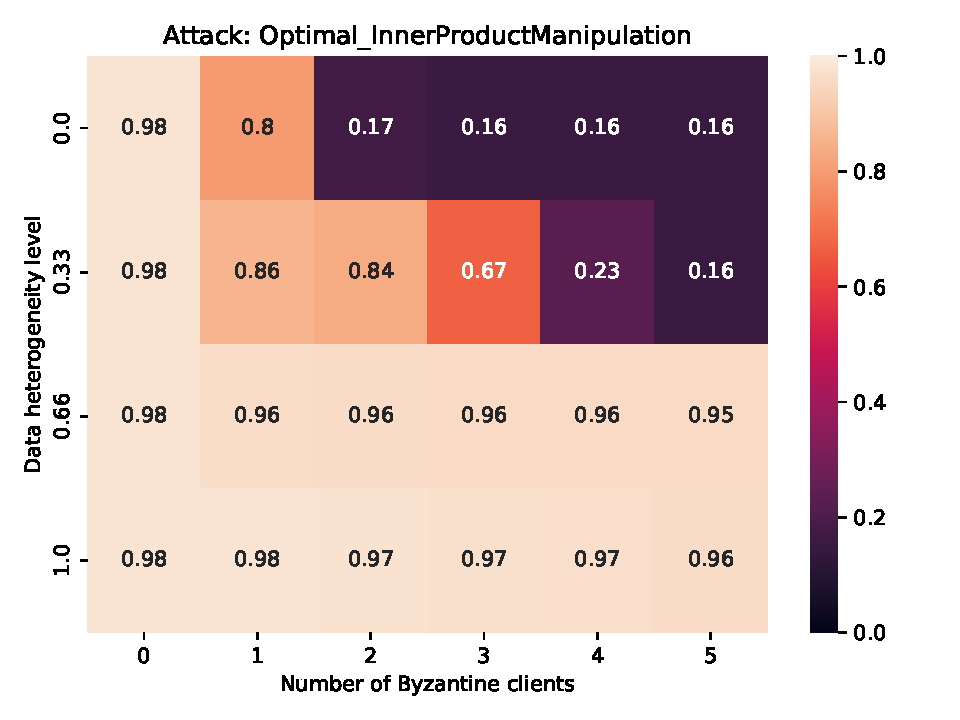
\includegraphics[width=\textwidth]{../plots/mnist_clipping_heatmaps/cnn_mnist_clipping_2/test_Optimal_InnerProductManipulation_mnist_cnn_mnist_clipping_2_gamma_similarity_niid_NNM_ARC_TrMean_nb_honest_clients_10_tolerated_f_equal_real.pdf}
        \caption{Hardtanh $C{=}2$}
        \label{fig:tm_ipm_hardtanh_2}
    \end{subfigure}
    \hfill
    \begin{subfigure}[b]{0.32\textwidth}
        \centering
        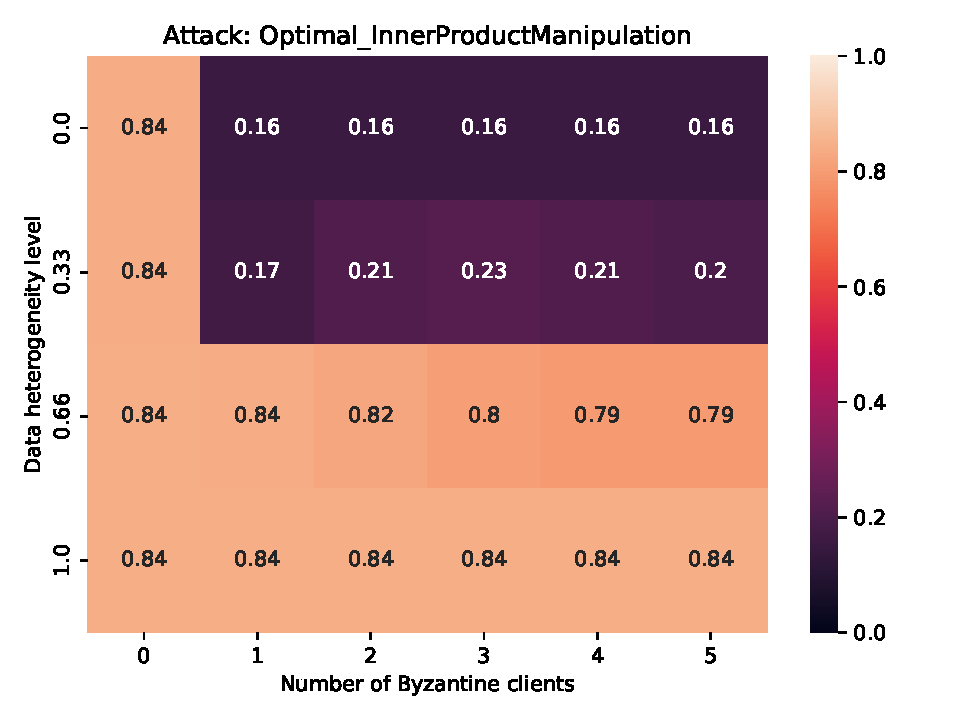
\includegraphics[width=\textwidth]{../activation_clip_plots/cnn_mnist_clip_ste_1/test_Optimal_InnerProductManipulation_mnist_cnn_mnist_clip_ste_1_gamma_similarity_niid_NNM_ARC_TrMean_nb_honest_clients_10_tolerated_f_equal_real.pdf}
        \caption{STE $C{=}1$}
        \label{fig:tm_ipm_ste_1}
    \end{subfigure}
    \hfill
    \begin{subfigure}[b]{0.32\textwidth}
        \centering
        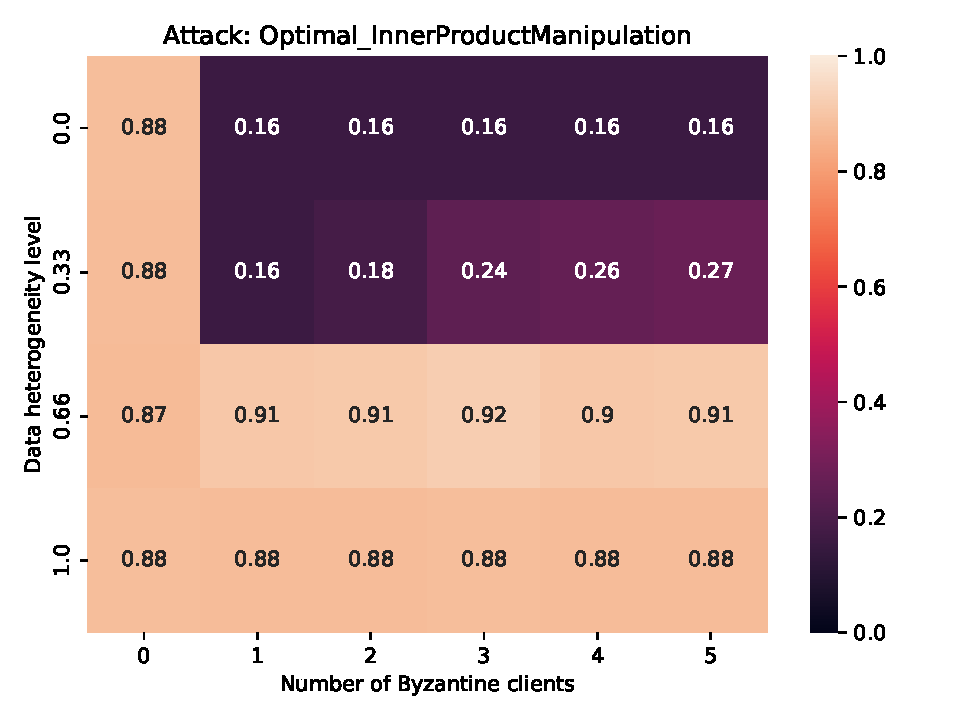
\includegraphics[width=\textwidth]{../activation_clip_plots/cnn_mnist_clip_ste_2/test_Optimal_InnerProductManipulation_mnist_cnn_mnist_clip_ste_2_gamma_similarity_niid_NNM_ARC_TrMean_nb_honest_clients_10_tolerated_f_equal_real.pdf}
        \caption{STE $C{=}2$}
        \label{fig:tm_ipm_ste_2}
    \end{subfigure}
    \vspace{0.3cm}
    \begin{subfigure}[b]{0.32\textwidth}
        \centering
        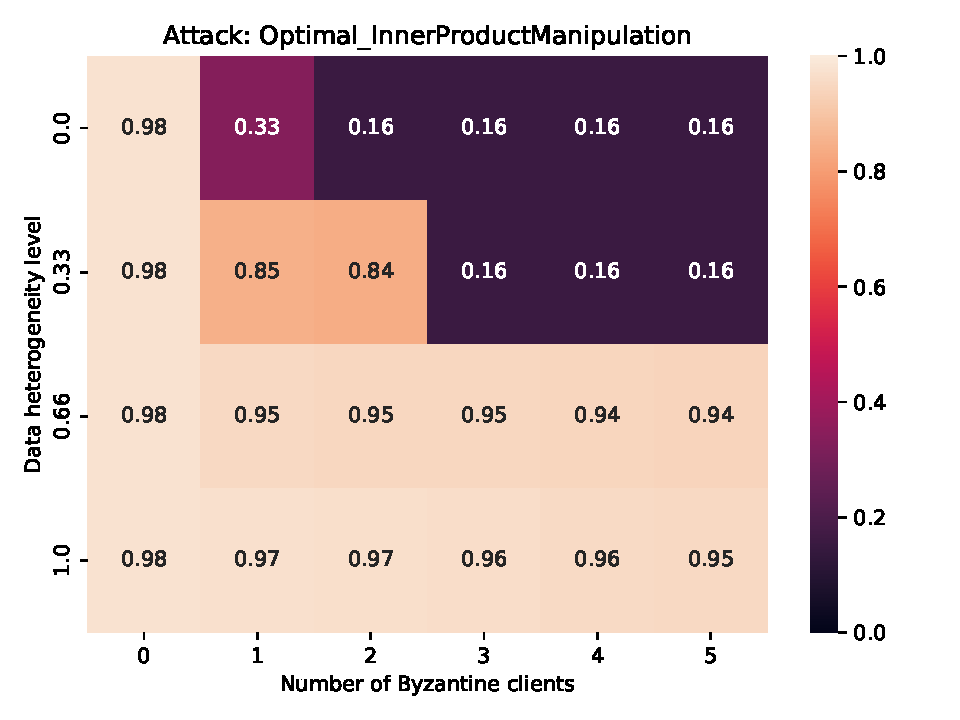
\includegraphics[width=\textwidth]{../activation_clip_plots/cnn_mnist_clip_ramp_1/test_Optimal_InnerProductManipulation_mnist_cnn_mnist_clip_ramp_1_gamma_similarity_niid_NNM_ARC_TrMean_nb_honest_clients_10_tolerated_f_equal_real.pdf}
        \caption{Ramp $C{=}1$ ($r{=}2$)}
        \label{fig:tm_ipm_ramp_1}
    \end{subfigure}
    \caption{Trimmed Mean (TM) under Optimal IPM Attack.}
    \label{fig:tm_ipm_grid}
\end{figure}
\clearpage

\end{document}
